\documentclass[twoside,a4paper]{article}

\usepackage[margin=2cm]{geometry}
\usepackage{amsmath,amsthm,amssymb,latexsym}
%\usepackage[v2,tips,curve]{xy}
\usepackage{graphicx}
\usepackage{backref, showkeys}

\theoremstyle{plain}
\newtheorem{proposition}{Proposition}[section]
\newtheorem{theorem}[proposition]{Theorem}
\newtheorem{corollary}[proposition]{Corollary}
\newtheorem{lemma}[proposition]{Lemma}
\theoremstyle{definition}
\newtheorem{definition}[proposition]{Definition}
\newtheorem{remark}[proposition]{Remark}
\newtheorem{example}[proposition]{Example}
\newtheorem{conjecture}[proposition]{Conjecture}

\newcommand{\mc}{\mathcal}
\newcommand{\rd}{\textrm{d}}

\begin{document}

\large
\title{An overview of self-excited point process models of crime}
\author{Matthew Daws}
\maketitle

\begin{abstract}
To do.
\end{abstract}


\section{Introduction}

Crime can spread through spacial locations and across time in a contagion-like way,
\cite{johnson}, and that after a (for example, property) crime is committed, there is
a spatially- and time-limited increased risk of further crime, \cite{jbberrt}.  At
the same time, there is an underlying spatial variation that may not change much with time,
\cite{johnson, bn}.  There has long been an interest in mapping variations in crime rate
to discern patterns, \cite{glv}.  More recently, there has been much interest in using
the repeat, or near-repeat, pattern of crime to predict future crime events, \cite{glv, jb, rand}.
A broad class of prediction techniques come under the heading of ``prospective hot-spotting'',
\cite{bjp, jbmbp}, where we estimate risk at the current time by looking at recent,
nearby crime events.  More formally, this is a kernel density estimation (KDE) method,
with an additional weighting by time.

In such techniques, it is necessary to have an \emph{a priori} choice of the kernels, and
bandwidths, to use in space and time.  Furthermore, there is no formal statistical model
in evidence.  Building on work in the theory of seismology, \cite{ml, vs, zovj}, there has
been much recent interest in ``self-exicited point processes'', \cite{mohler, sepp, sepp2, rc}.
Here we have an explicit statistical model, either parametric or non-parametric, and
we proceed in a standard way to fit this model to data, and then to use the model to make
predictions.  We note that there has been surprisingly little discussion in the literature
about how \emph{exactly} to make predictions based on this class of model; see
Section~\ref{sec:making_preds} below for further discussion.
It is widely believed that, in particular, \cite{sepp2} is the basis of the algorithm
employed by the commercial crime prediction package PredPol, \cite{predpol}.

These techniques are attractive as they combine explicit statistical models with techniques
for fitting these models to data.  This allows us to both make inferences based upon the
data, \cite[Section~4]{sepp}, and to make predictions, \cite[Section~5]{sepp}, \cite{sepp2, rc}.
However, the relatively sophisticated mathematics, and in our view the slightly
opaque presentation of the algorithms involved, may pose a barrier to entry into this field.

We have three aims in this paper.  While \cite{sepp2} mentions the EM algorithm by name,
\cite{sepp} does not, and it is far from clear from the majority of papers in this area
that all of the algorithms are actually variants of the Expectation Maximisation (EM)
algorithm, \cite{mk}, and that it is possible to rigorously derive all of the
specific algorithms from this one technique.  We carefully show have the technique of the
EM algorithm can be applied to each specific model we develop.

This work came about as part of our efforts to build an open source, Python based
implementation of different crime prediction algorithms, which forms the \texttt{open\_cp}
package.\footnote{Available at \texttt{https://github.com/QuantCrimAtLeeds/PredictCode}}
The current paper is backed by Python code
[\footnote{Eventually, link to public repo.}]
which implements each model.  We use the framework provided by \texttt{open\_cp}, and base
classes which abstract typical EM algorithm code.  It is our hope that this open source
framework, together with our development of the theory, will make it easier for other
researchers to both reuse and reproduce our work, and also allow others to develop, more
easily, their own models.

Finally, we have found that while the implementation of existing algorithms in
\texttt{open\_cp} work well with artificial data, generated from the statistical model,
running such algorithms on real-world data is fraught with problems.  This is alluded to
in \cite{rc} as well.  In this paper we discuss theoretical reasons for the problems we
have observed, and suggest new models which perform more robustly.  Having a well-developed
understanding of the probability theory behind these algorithms has been crucial in gaining
these insights.


\subsection{Acknowledgements}

This work was funded by the UK Home Office Police Innovation Fund, through the
project ``More with Less: Authentic Implementation of Evidence-Based Predictive
Patrol Plans''.  The author wishes to thank Gabriel Rosser, Kristian Lum, William Issac,
and Martin Short for useful electronic correspondance.



\section{Point process models}

For general background on point processes, see the mathematical \cite{dvj}; the
introductory lecture notes \cite{ras}; the gentle introduction in \cite[Chapter~8]{rip},
or the encyclopedic \cite{handbookss}.

We shall view crime events as point events in time and space, say $N$ events which occur
at times $t_1 < t_2 < \cdots < t_N$ and at locations $(x_i, y_i)_{i=1}^N$ which are all
distinct.  The ``distinct'' condition is important is important because of the
mathematical abstraction we use, but we could model exact repeats using \emph{marks};
see also the discussion in Section~\ref{sec:exact_repeats} below.
Alternatively, we can assign points to cells in a spatial grid
(\cite{sepp2}) and/or bin timestamps to intervals of time (see again
Section~\ref{sec:exact_repeats} below).
As noted in \cite[Part~V]{handbookss} while we can treat time as just another dimension,
and work with ``spatial'' point processes in $\mathbb R^3$, for motivation, and interpretting
results, it makes more intuitive sense to work with time as being different.  We shall
continue to assume that time is ordered, flowing from the past to the future.
A more sophisticated way to treat time is via ``aoristic analysis'', \cite{ratcliffe},
treating times as being probabilistic \emph{time ranges} instead of exact times; however,
we shall not consider this added complication here.

We shall only consider point processes which admit an \emph{intensity function},
Appendix~\ref{app:pp}.  Informally, we consider a function $\lambda^*(t,x,y)$ which gives
the probability of an event occurring in an infinitesimal volume around the point $(t,x,y)$.
A useful interpretation is that for any region $V$ of space time, if
\begin{equation}
\lambda(V) = \int_V \lambda^*(t,x,y) \ dt \ dx \ dy,
\label{eq:exp_poisson}
\end{equation}
and we define $N(V)$ to be the number of events we observe in $V$, then $N(V)$ will be a
random variable distributed as a Poisson distribution with mean $\lambda(V)$.  If $U$ is
another space time region disjoint from $V$, then $N(V)$ and $N(U)$ are independent random
variables.

For example, a homogeneous Poisson process has $\lambda^*$ being constant.  An inhomogeneous
Poisson process has $\lambda^*$ being a genuine function (compare the discussion below).
We might, for example, model the time dependence as $f(t)$, perhaps using tools from time
series analysis, and model space dependence as $g(x,y)$, maybe using a KDE method, by setting
$\lambda^*(t,x,y) = f(t) g(x,y)$.

The models we shall be interested in are ``self-excited'', which loosely means that the present
behaviour of the process will depend upon its history.  This explains our use of the $*$ in
the notation $\lambda^*$ which reminds us on the dependence on the history of the process.
Indeed, our models will always be of the form
\[ \underbrace{\lambda^*(t,x,y)}_{\text{Total intensity}}
= \underbrace{\mu(t,x,y)}_{\text{Background rate}}
+ \underbrace{\sum_{t_i < t}}_{\parbox{1.1in}{\footnotesize Sum over events \emph{before} the current time}}
\underbrace{\mu_1(t-t_i, x-x_i, y-y_i)}_{\text{Triggering intensity}}. \]
Thus $\lambda^*$ depends upon the \emph{history} of the process, the events $(t_i,x_i,y_i)$
with $t_i<t$, where $t$ is the current time.  $\mu$ is a genuine function, specifying the
background rate or intensity, which is the rate at which events occur ``just by
chance''.  Each time an event at time $t_i$ occurs, it adds (linearly) extra intensity
governed by the ``triggering'' intensity $\mu_1$.  Notice that $\mu_1$ only depends upon
the distance, in space and time, between the event and position of interest $(t,x,y)$.

We could consider more general $\mu_1$, which also depended upon $(t,x,y)$, and indeed there
might be good reason for doing so (perhaps to model a more spatially concentrated
triggering in a densely populated area of a city, vs a spatially disperse triggering
in a suburban setting).  However, we shall find that fitting the simpler model is
currently enough of a challenge, and leave this extension for future research.

The classical prospective hot-spotting technique, \cite{bjp}, can be thought of as a model
of this form, where $\mu=0$ identically, and $\mu_1$ is chosen ahead of time.  An
advantage of the models considered in \cite{sepp, sepp2} is that they allow $\mu$ to be
non-zero, and that they use \emph{past data} to inform the shape of $\mu$ and $\mu_1$.

The EM algorithm is an iterative algorithm which seeks to find Maximum Likelihood estimates
of parameters (there are extensions to other applications) for models which admit ``hidden
variables'' or ``unobserved data''.  A classical example is a \emph{censored} experiment:
perhaps we know how long patients lived who were treated with a variety of treatments, except
that if a patient lived for the entire study duration then we only know that
they lived \emph{at least} that long.  We would typically model this as letting $Z_i$ be
the random variable which is survival time, but we only observe $Y_i = \min(Z_i, T)$ for
some fixed $T$.  The EM algorithm can also be applied to models where the hidden variables
are merely useful mathematical constructs added to simplify analysis.

A useful way to \emph{simulate} a process (compare the introduction of \cite{mr, mr1})
of our form is to exploit the hidden
\emph{branching structure} of the process, which exists because the triggering
kernel is linear.  We first simulate an inhomogeneous Poisson process with intensity $\mu$,
giving the ``background events''.  Then for each background event $i$, we start at time $t_i$
and simulate a new inhomogeneous Poisson process with intensity $\mu_1(t-t_i, x-x_i, y-y_i)$.
We then translate this process by space time position $(t,x,y)$, and add the points into our
collection.  We consider these to be ``triggered events'' which have been ``triggered by $i$''.
We now look at all the new points, and continue the process.  As each new point
is created into the future, and we only wish to simulate a finite interval of time, our
simulation will eventually end.  (We note that we might also somehow ``simulate into the past'',
as events before time $0$ might trigger events after time $0$.  Such considerations lead to
the concept of a ``perfect simulation'', see \cite{mr}).

Let $z_i$ be the event which ``triggered'' event $i$, with the convension that if $z_i=i$
then $i$ is a background event.  Thus $z_i \leq i$.  The $(z_i)$ form our unobserved data.
The EM algorithm then works by using the current estimate of the parameters to assign a
probability to the event $z_i=j$ for all $i$ and $j$.  The $E$ step computes the conditional
expectation of the log likelihood, conditional over the hidden data $(z_i)$.  The $M$ step
then maximises the parameters given this conditional expectation.  The idea is that if
we \emph{knew} the values of $(z_i)$, we could replace the $E$ step by simple evaluation,
and then the $M$ step would be the usual maximum likelihood estimation.
The EM algorithm can be proved to converge to a \emph{local maximum} under mild conditions,
and the beauty of it is that in many practical applications, the resulting procedure is
computationally tractable.

We give further details in Appendix~\ref{app:pp} and~\ref{app:em}, but summarise the
resulting family of algorithms here.  Let $p_{j,i}$ be the probability that event $j$
triggered event $i$, for $j\leq i$.  We have
\[
p_{j,i} = \mathbb P(z_i=j) = \begin{cases}
\mu(t_i,x_i,y_i) / \lambda^*(t_i,x_i,y_i) &: j=i \\
\mu_1(t_i-t_j, x_i-x_j, y_i-y_j) / \lambda^*(t_i,x_i,y_i) &: j<i
\end{cases}
\]
Notice that then $\sum_j p_{j,i} = 1$ for each $i$.

Let $\mu(t,x,y) = \mu(t) f(x,y;t)$ be a factorisation, where we suppose that always
$f$ is a probability density, so $\int_{\mathbb R^2} f(x,y;t) \ dx \ dy = 1$ for all $t$.
For many models, $f$ will not depend upon time and so $f(x,y;t) = f(x,y)$ will simply be
a function of $x,y$.  Similarly let $\mu_1(t,x,y) = \mu_1(t) g(x,y;t)$.  Then $\mu_1$
governs the rate of triggering, and to stop a runaway process, we must have that
$\int_0^\infty \mu_1(t) \ dt < 1$.

The log likelihood, given $(z_j)$, is
\begin{align*}
\log L &= \sum_j \log\Big(\mu(t_j) f(x_j,y_j;t_j)) [z_j=j] \\
&+ \mu_1(t_j - t_{z_j}) g(x_j - x_{z_j}, y_j - y_{z_j};t_j - t_{z_j}) [z_j<j] \Big) \\
&- \int_0^T \mu(t) \ dt - \sum_{j=1}^n \int_0^{T-t_j} \mu_1(t) \ dt,
\end{align*}
where $[\cdot]$ is the Iverson bracket, so for example $[z_j=j]$ is a random variable,
equal to $1$ is $z_j$ is $j$, and $0$ otherwise.  The integrals are essentially
normalisation factors.

This sum may look formidable, but we can use two tricks.  Firstly, the $E$ step
computes the conditional expectation, and we can use the \emph{linearity} of
the expectation.  See equation (\ref{eq:two}) in the appendix, for example.
Secondly, at the maximisation step, we have parameters we wish to maximise, and typically
will take partial derivatives and solve for when the derivates are zero.  Differentiation
is also linear, and so commutes with the expectation.  Unfortunately, we have not been
able to find a simple recipe that translates the EM algorithm into a general procedure,
at least at this level of generality.  However, for any given model, it is typically
rather simple to follow the EM algorithm.

We also note that in the point process (see \cite[page~1402]{sepp2} for just one example)
literature, one often finds algorithms with steps labelled the ``E step'' and ``M step'',
but, comparing with our derivations in the appendix, these really do not have much to do
with the ``E'' and ``M'' steps of the (abstract) EM algorithm.  We will avoid such terminology.


\subsection{Hawkes processes}

Suppose we ignore any spatial component, so the intensity is
\[ \lambda^*(t) = \mu(t) + \sum_{t_i<t} \mu_1(t-t_i). \]
The original Hawkes process takes $\mu(t)=\mu$ to be constant, and sets $\mu_1$ to
be exponential decay, say $\mu_1(s) = \theta \omega e^{-\omega s}$.  Such models have
been long studied by the financial Mathematics community, see the nice overview \cite{ltp},
for example.  It is worth noting that \cite[Section~4]{ltp} warns of the complexity and
difficulty of fitting such models to real data: we of course are trying to fit much more
complicated models to data!  We have found that thinking about Hawkes processes is
a great way to understand the more complicated, spatial models this paper develops.
The lecture notes \cite{ras} are a gentle and useful introduction.

The paper \cite{lm} develops the EM algorithm as applied to a Hawkes process; we
repeat this derivation, with further details, in Appendix~\ref{app:hawkes_em}.
In \texttt{open\_cp} we implement this model, and recreate the work leading to
\cite[Figure~1]{lm}.  This demonstrates one of the problems with parameter estimation here:
when the ``clusters'' coming from the trigger function are dispersed (so $\omega^{-1}$ is
large, relative to $\mu^{-1}$) it can be very hard to distinguish background events from
triggered events.  Indeed, our recreation of \cite[Figure~1]{lm} typically
fails\footnote{See \texttt{https://github.com/QuantCrimAtLeeds/PredictCode/blob/master/notebooks/sepp\_2\_testbed.ipynb}}
when $\omega^{-1}=10$.



\section{Trial data}

We illustrate the models by using open crime data available from the city of Chicago,
\cite{cdata}, as used in \cite{rc}.  See Figure~\ref{fig:chicago_overview} for example
plots of the data.  We explore this dataset in detail in \cite{daws1} where we argue
that the coordinates are only approximate, and are deliberately clustered to anonymise
location.  We downloaded this dataset in 2017, while \cite{rc} used an earlier version of
the data which displays slightly different location clustering, see the plot in \cite{rc}
and the extended discussion in \cite{daws1}.

\begin{figure*}
  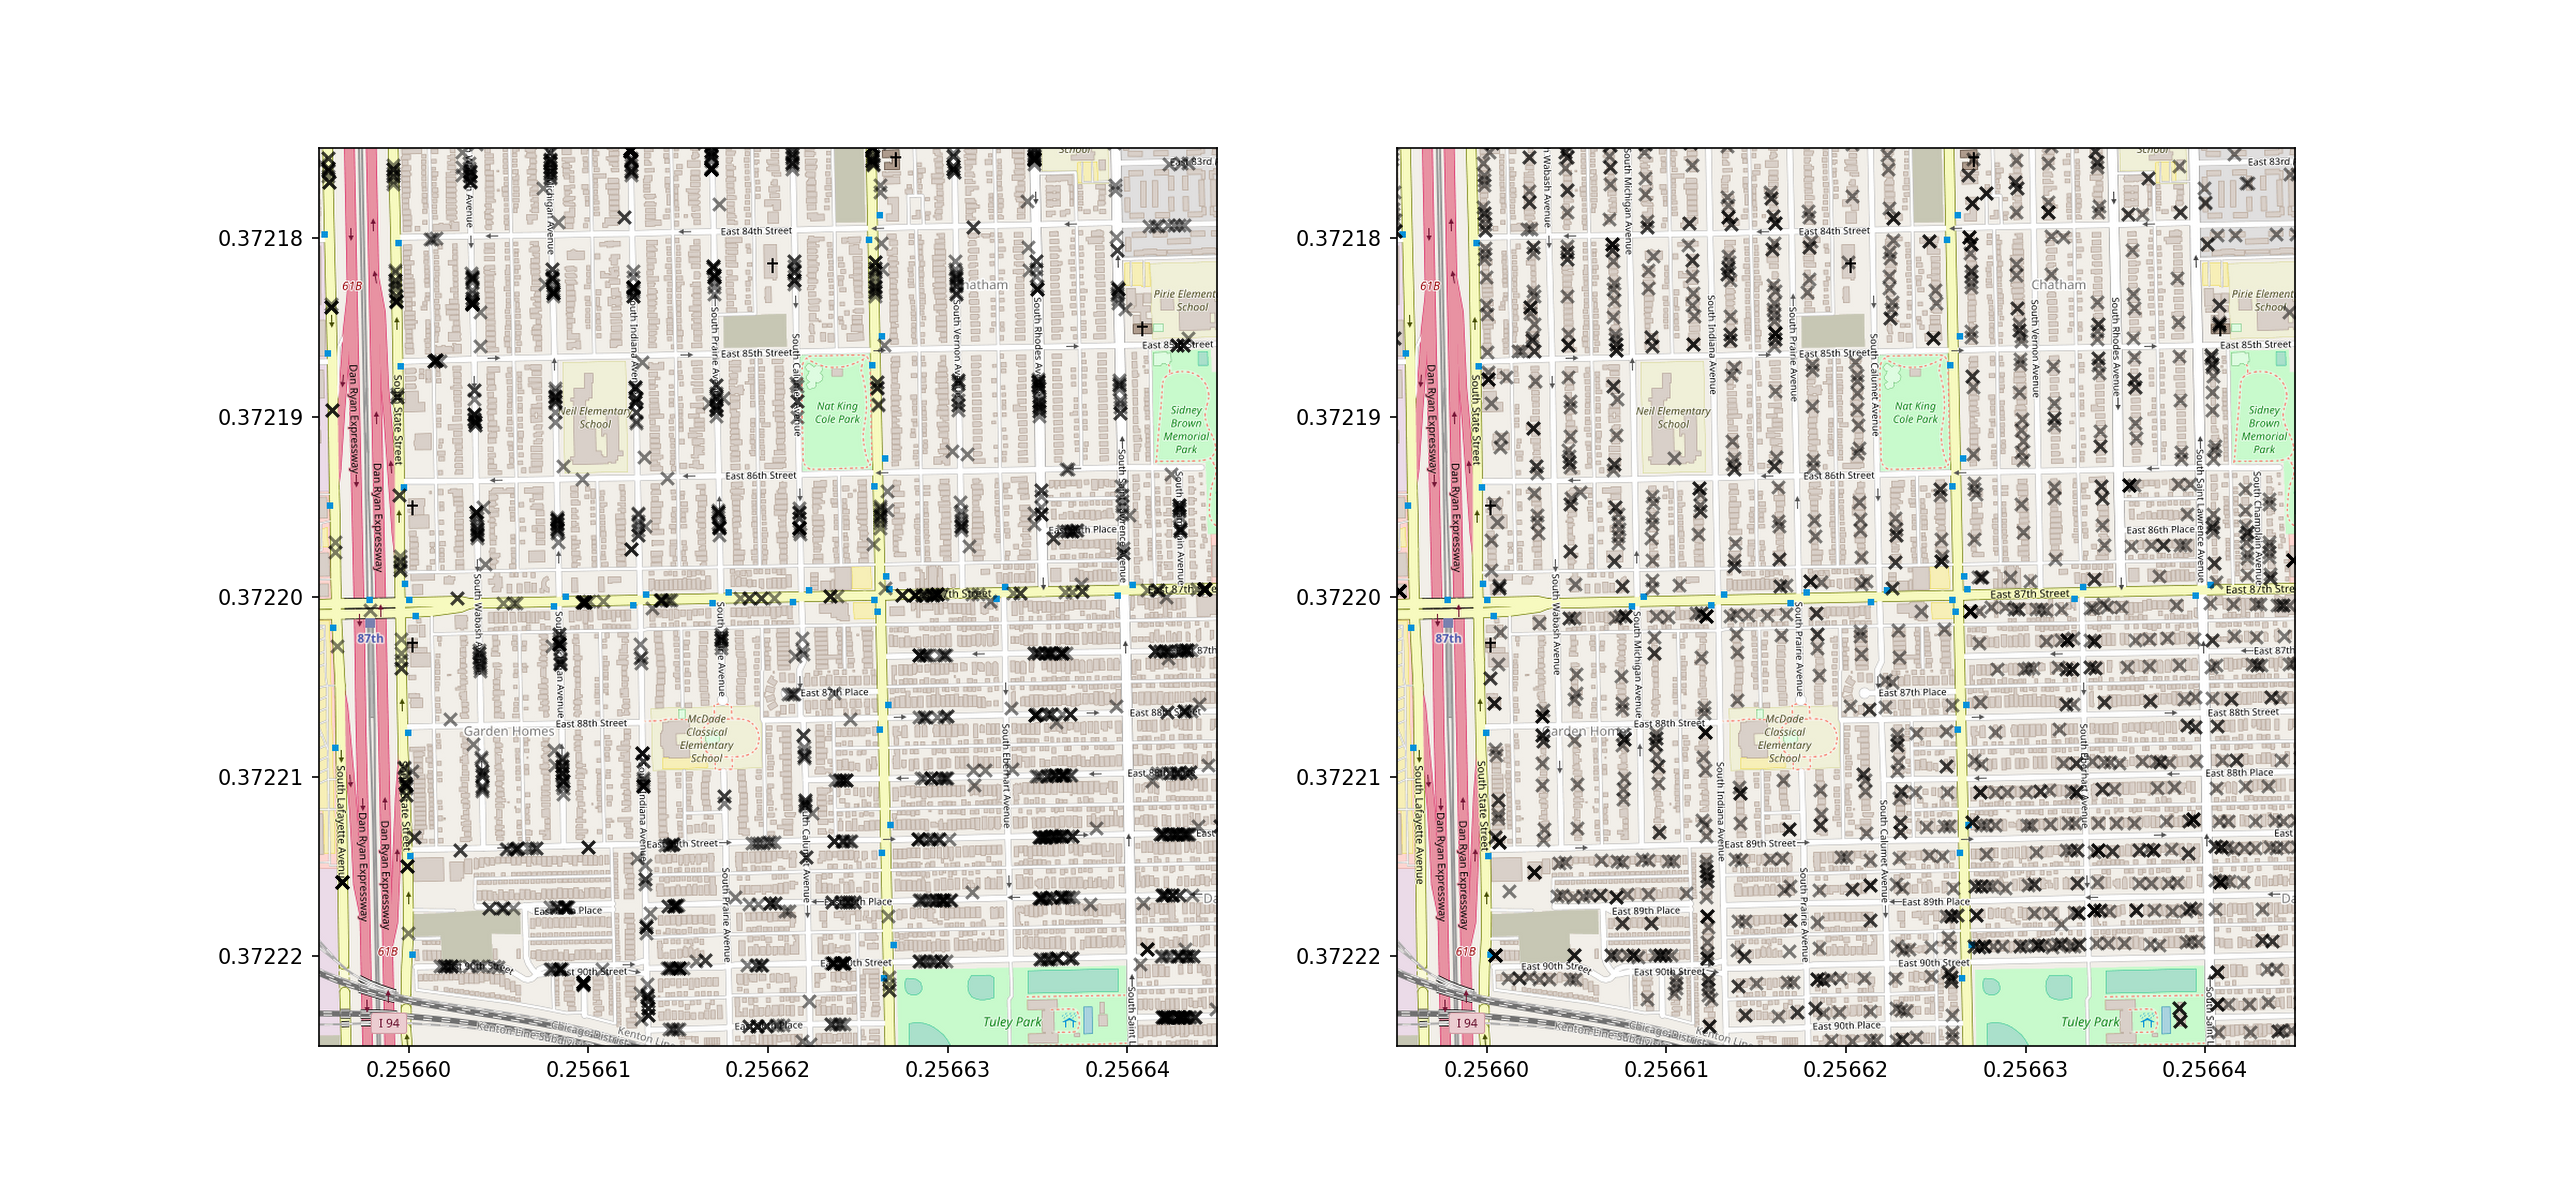
\includegraphics[width=\textwidth]{../notebooks/Chicago_overview.png}
  \caption{A section of the Chicago data: notice the clustering of events along city
  streets in the left-hand plot.  The right-hand plot shows artificially ``redistributed''
  points, each aligned to a building.  Here and in the rest of the paper, we look only at
  Burglary crime, and mostly focus on the North side of Chicago.}
  \label{fig:chicago_overview}
\end{figure*}

Given that this data is artificially clustered, we also use ``redistributed'' data from
\cite{daws1}. The original points have been moved a small distance around the street network,
and then assigned to the nearest building (see \cite{daws1} for a fuller discussion).
Police data in the UK, especially for Burglary events, is often geocoded to buildings, and so
we hope this second dataset will be more representative (at least certain sorts) of real-world
data.



\section{Grid based models}\label{sec:gbm}

The model in \cite{sepp2} is a grid-based, parametric model, for which the EM
algorithm is easier to motivate.  The model considers a grid laid over the study area,
and in each grid cell $k$ we assume that we have a Hawkes-like model, which is independent
of other grid cells.  Thus, if events in cell $k$ occur at times $t^{(k)}_1 < 
t^{(k)}_2 < \cdots < t^{(k)}_{n(k)}$ then the intensity for cell $k$ is
\[ \lambda^*_k(t) = \mu_k + \sum_{t^{(k)}_i < t} \theta \omega
e^{-\omega(t-t^{(k)}_i)}. \]
Notice that the background rate $\mu_k$ do not vary in time, but does depend on the cell $k$,
while the triggering parameters $\theta$ and $\omega$ are assumed to be constant in both time
and grid cell $k$.  Appendix~\ref{app:grid_model_em} presents a careful derivation of
the full EM algorithm in this case, and explains the assumptions which lead to the simplified
algorithm presented in \cite[Section~2.2]{sepp2}.

This algorithm is implemented as the \texttt{seppexp} module in \texttt{open\_cp}.
The \texttt{sources.sepp} module in \texttt{open\_cp} allows simulating (using a ``non-perfect''
simulation method) data from these types of model.  We simulated data from this
specific model with $\theta=0.5, \omega=10$ and with $\mu_k$ randomly chosen uniformly
from $[0,1]$.  Using either the full EM algorithm, or the simplified algorithm, we
estimate $\theta=0.51, \omega=8.9$ and obtain a good match with $\mu_k$, see
Figure~\ref{fig:sim_grid}.  However, with $\theta=0.5, \omega=0.1$, we estimate $\theta=0.2$
and $\omega=0.65$, and from Figure~\ref{fig:sim_grid} we see that the background rate
is over-estimated.  That is, a maximum likelihood approach over-estimates the number
of background events.  We see no difference between the simplified EM algorithm (which assumes
no ``edge effects'') and the full algorithm.

\begin{figure*}
  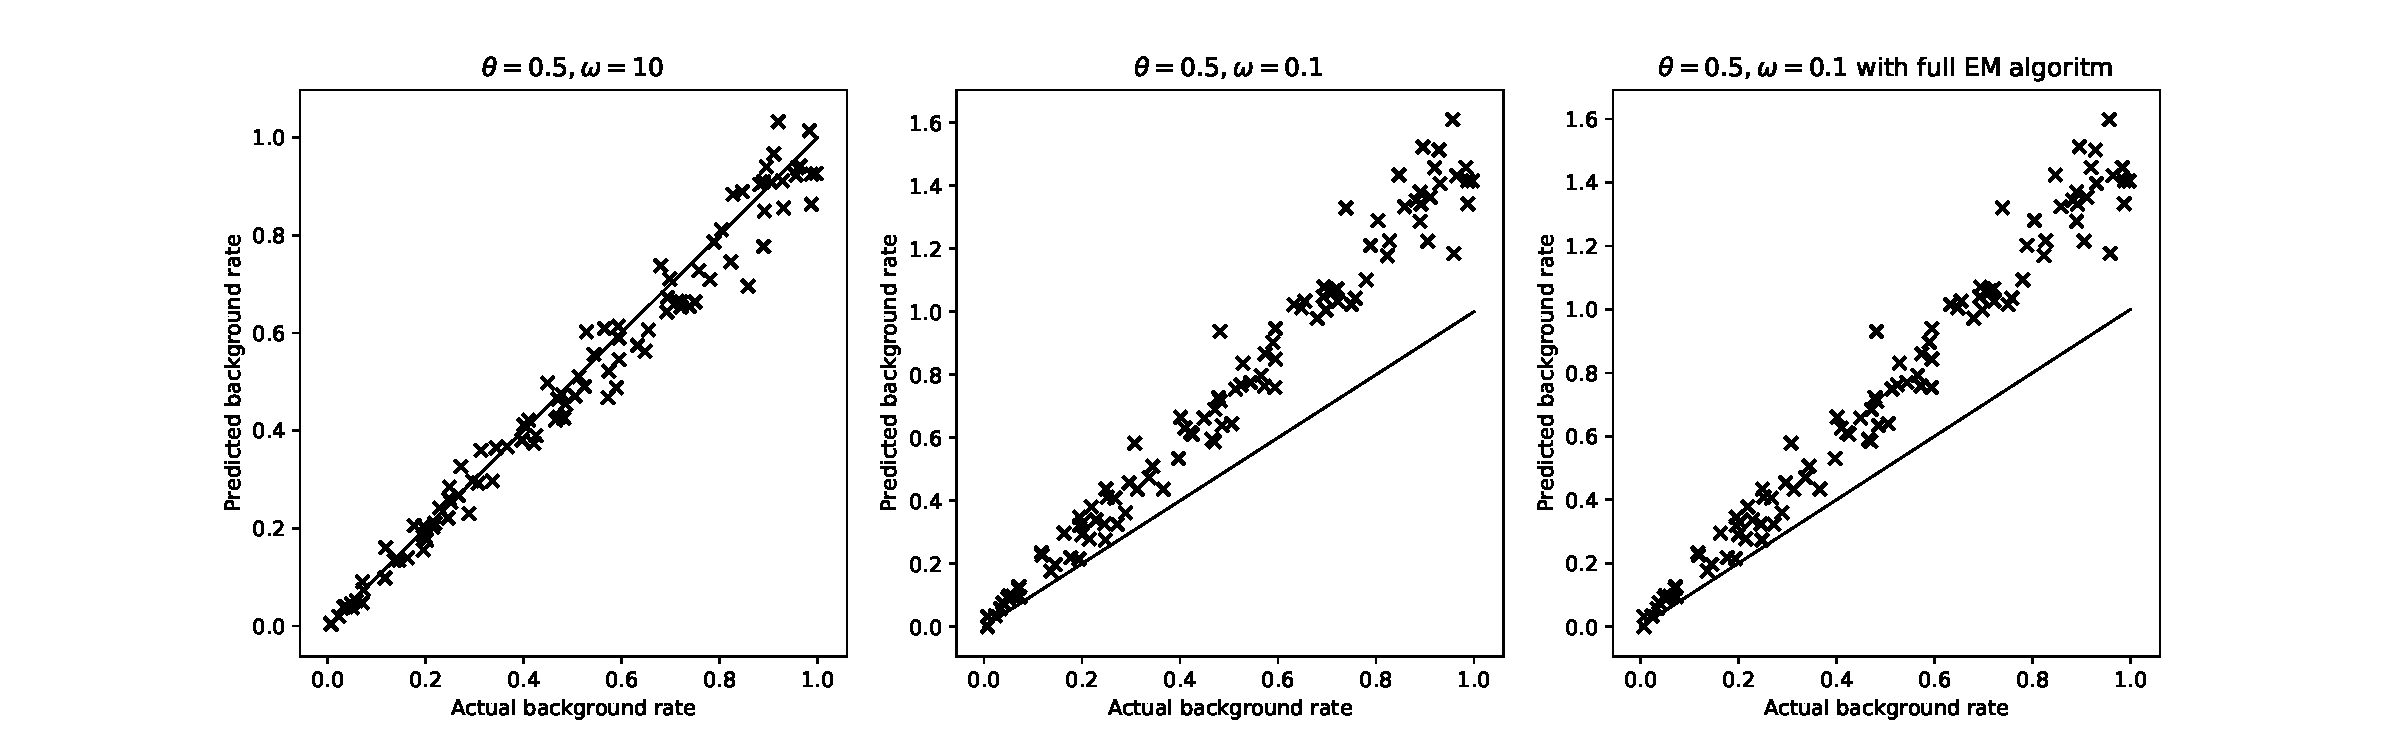
\includegraphics[width=\textwidth]{../notebooks/simdata.pdf}
  \caption{Fitting the grid based model to simulated data, Section~\ref{sec:gbm}.}
  \label{fig:sim_grid}
\end{figure*}

Unfortunately, we have not been able to obtain sensible results from this algorithm
as applied to real data.  The algorithm converges without issue, but seems to always
report completely unrealistic triggering parameters.  We use Burglary crime events
from 2016 for the North side of Chicago, with a grid size of 150m, as in \cite{sepp2}.
The model predicts $\theta = 2.13 \times 10^{-2}$
and $\omega = 18.32$, with a time unit of one day, so that $\omega^{-1} \approx 79$
minutes.  The background rate has a maximum of $2.73\times 10^{-2}$, so that $\theta$ is
comparable to the background rate.  This means that the triggering kernel gives an
elevated risk above background for only a matter of hours.  This seems unrealistic, as
previous studies, \cite{jb}, considered an increased risk of (near-)repeat burglary
on the order of days or weeks.

Similar behaviour (with only a slightly longer value for $\omega^{-1}$) is shown for
the second dataset.
We have repeated the study using the different regions of Chicago, and have obtained
similar results for all, with the exception of the ``Far Southwest'' which has $\omega^{-1}$
of about 10 hours, and the ``Southwest'', where the algorithm fails to converge.
Running the algorithm on other year's worth of data shows similar behaviour.

This failure of convergence is due to a problem which we will meet again below, so it
is worth exploring now.  The log likelihood of the total data is
\[ \sum_{k,i} \log\Big( \mu_k + \sum_{j<i} \theta\omega e^{-\omega(t^{(k)}_i - t^{(k)}_j)} \Big)
- \sum_k T\mu_k - \sum_{k,i} \theta(1-e^{-\omega(T-t^{(k)}_i)}), \]
(compare with Appendix~\ref{app:pp}).  Suppose that there exists $k$ and $j<i$ with
$t^{(k)}_i = t^{(k)}_j$.  Then we have a term which is
\[ \geq \log\Big( \mu_k + \theta \omega e^{-\omega(t^{(k)}_i - t^{(k)}_j)} \Big)
\geq \log( \theta\omega \big), \]
as $e^0 = 1$.  We have a further summand which is negative and scales with $\theta$, 
but no such ``correction'' for $\omega$, and so as $\omega\rightarrow\infty$ the
likelihood increases without bound.  We find that the EM algorithm does exactly this:
it estimates $\omega$ to be larger and larger until a numerical error occurs.

If we change the data by adding small random numbers to the timestamps (while maintaining
the ordering) then the problem disappears.  Examining the input data, we do indeed find
some exact repeats: these might be data errors, or they could be due to the fact that
timestamps are only approximate, and that the geocoding is partly anonymised.

This occurs because, throughout, we work with \emph{simple} point processes throughout,
see the discussion in \cite[Section~8.2.7]{cressie} for example; as \cite{cressie}
notes, we could deal with this through \emph{marked} point processes, the mark giving how
many repeats occurred at that time and place.  This seems like an unnecessary complication
which we have not seen explored elsewhere.

There are two possible problems with this model.  Firstly, as we saw in the simulation study,
when the actual value of $\omega$ is small, we can significantly over-estimate both
$\omega$ and the background rate.  Secondly, the model does not model interaction between
grid cells, while clearly there is every chance of a burglar moving between different cells.
We deal with the second objection in later sections; the first issue seems harder to address.


\subsection{Understanding the repeat rate}

Above, we found a small value of $\theta$, and compared it to the background rate.
An arguably better way to interpret $\theta$ is as follows.  Each event adds a new trigger
kernel at its location, and the total intensity of the trigger, which is $\theta$, is exactly
the expected number of new events the trigger will give rise to.  As each of these events
will give rise to further triggers, the total number of expected events, in total, which one
event will subsequently trigger is
\[ \mu + \mu^2 + \mu^3 + \cdots = \frac{\mu}{1-\mu}. \]
See Appendix~\ref{app:gen_func} for a rigorous argument.  For example, with $\theta=2.13
\times 10^{-2}$ found above, we expect each event to trigger $2.18\times 10^{-2}$ further
events (that is, essentially none!)


\subsection{With a truncated exponential kernel}

If exact repeats in times can cause the estimaton of $\omega$ to diverge to $\infty$,
then we might worry that different, but rather close, timestamps might cause $\omega$ to
be estimated larger than is reasonable.  A small change we can make to the model to is
replace the ``triggering'' kernel $\omega e^{-\omega t}$ with 
\[ g(t) = \begin{cases} 0 &: t<t_0, \\ \omega e^{-\omega(t-t_0)} &: t\geq t_0.
\end{cases} \]
This corresponds to ``inhibiting'' triggering from happening between events which are
$<t_0$ in time apart.  The details are worked out in Appendix~\ref{app:grid_model_em_inhib}.

Again, on real data, this technique does not appear to work well.  While we sometimes
see $1/\omega$ get larger (e.g. the order of days) this is accompanied by $\theta$ being
estimated as being vanishly small, suggesting almost no triggering effect.
The second dataset behaves in the same way.



\subsection{Allowing exact repeats}\label{sec:exact_repeats}

While our formal probability model does not allow exact repeats ($t_i=t_j$ with $i<j$),
as we briefly explain in Appendix~\ref{app:exact_repeats_in_time}, we can adapt the EM
algorithm to deal with such data.  This opens the door to ``binning timestamps'', which
from informal conversations with other researchers, is seemingly a data preparation task
which is often carried out.  There are perhaps good reasons for this, two of which are
that: firstly, if we are making predictions for, say, the following day, then we perhaps
should not be interested in exactly when a previous event occurred, only which day it
occurred on; and secondly, we perhaps do not quite believe the accuracy of timestamps in
our data (which are likely not really accurate to the nearest minute, for example).

Yet again, on real data, this technique does not appear to work well.  There is a lot of
sensitivity to exactly how we bin the timestamps (the length of the bins, and the offset
from which bins start).  Again, we often see that when $\omega^{-1}$ becomes large,
$\theta$ is estimated as being vanishly small, suggesting almost no triggering effect.
It is possible to ``tune'' the binning, on some datasets, but this begs the question of
how we implement a \emph{robust} method.

From looking at the input data, we do not notice anything in particular which would
obviously cause such a dependence on the offset of binning.  The number of events per day
is distributed much as a Poisson random variable, and the number of events per weekday
is fairly constant across the working week, and a little lower at the weekend.  The
only slight surprise is shown in Figure~\ref{fig:by_hour_of_day}, where we see that
for the North side of Chicago, there
are an unexpected large number of Burglary events timestamped to between 8am and 9am.
Otherwise the number of events is fairly constant across the day, with a slight dip
from 3am to 7am.  We do not know if, perhaps, people awake up and discover an overnight
burglary; or if events are logged at this time but actually happen early, perhaps due
to some sort of ``overnight working partern'' effect on behalf of the police (to give
just two plausible reasons).  Notice that we see somewhat different patterns for the
South and Southwest sides.

\begin{figure*}
  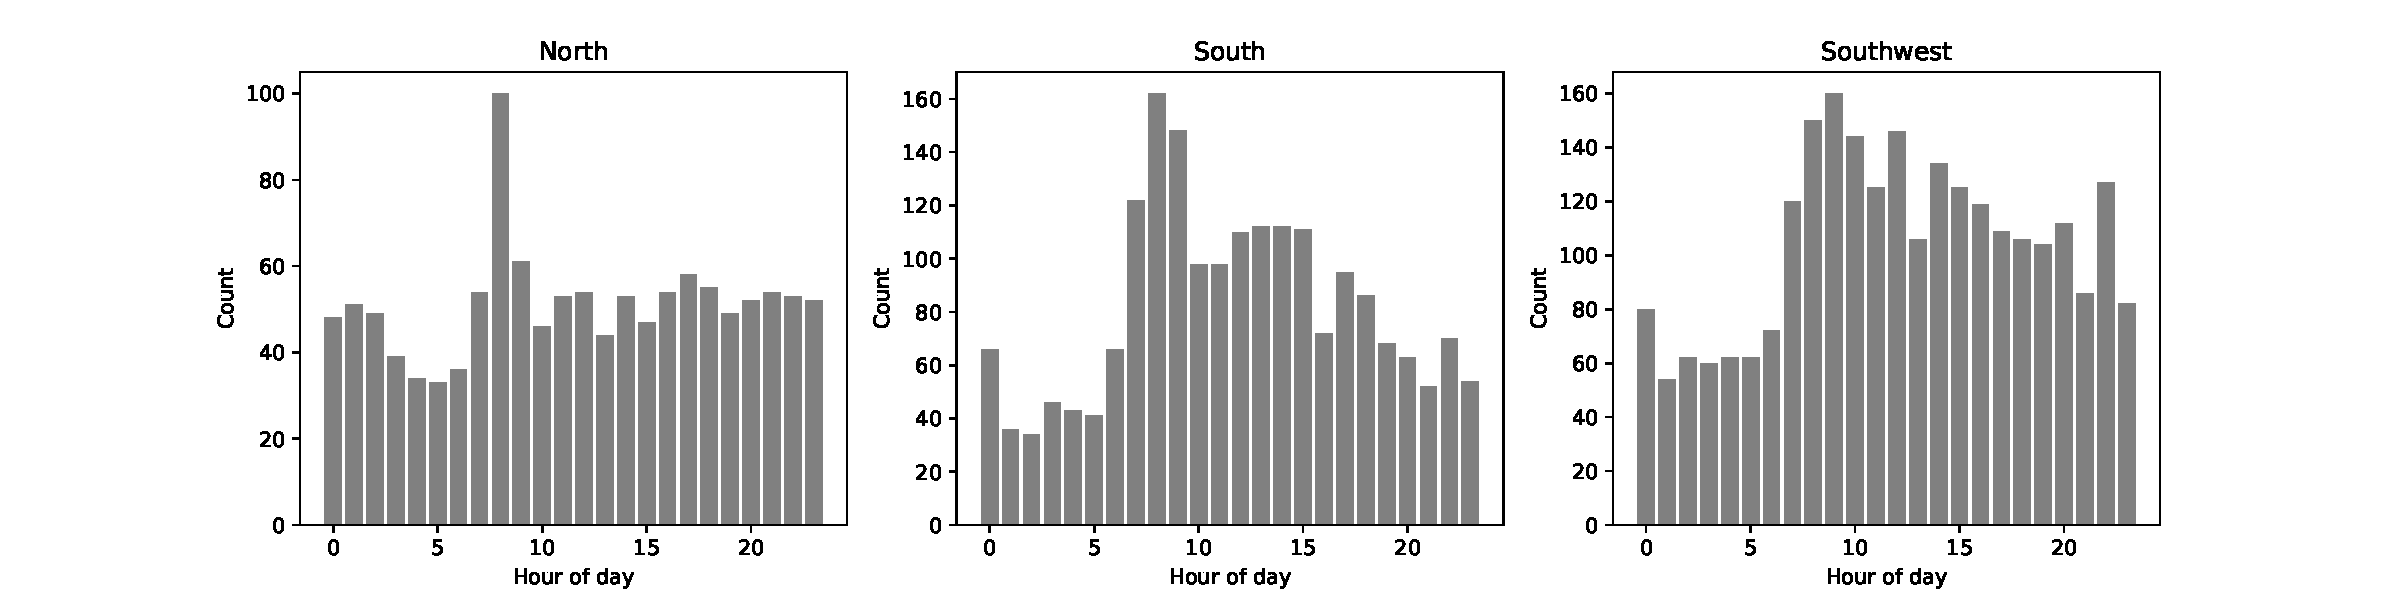
\includegraphics[width=\textwidth]{../notebooks/events_by_hour.pdf}
  \caption{For three sides of Chicago, data from 2016, for Burglary event,
the number of events per hour of the day.}
  \label{fig:by_hour_of_day}
\end{figure*}

Repeating the sort of experiment which lead to Figure~\ref{fig:sim_grid}, with $\omega=10$,
we find that binning the timestamps to the nearest hour works well, but that if we bin to
the nearest 6 hours interval, then we again tend to systematically underestimate the
background rate (that is, the effect is the same as making $\omega$ small).

There is no ``cost'' to allowing exact repeats, except for the tiny computational effort
of adjusting the $p$-matrix.  Henceforth, we shall allow exact repeats in time, for simplicity.





\section{Non-parametric grid based models}

Rather than assume a parametric form of the triggering kernel, we could instead take a more
``data driven'' approach, and use a non-parametric form for the triggering kernel.  We
explore this first for our grid based models, before later extending it to give a non-parametric
form for the background as well, and allowing interaction between different grid cells.




\subsection{A histogram estimator}

A first step in this direction is to consider a ``histogram estimator'', compare
\cite[Section~2.2]{sil}.  Already here, the details of putting this into the EM algorithm
are slightly non-trivial, see Appendix~\ref{sec:his_est}.  The particular model we use
is detailed in Appendix~\ref{app:grid_hist}.  We replace the exponential triggering kernel
$\omega e^{-\omega t}$ by the ``histogram''
\[ g(t) = \alpha_k \quad\text{if}\quad r\in\mathbb Z, rh \leq t < (r+1)h, \]
where $h>0$ is the \emph{bandwidth} and $(\alpha_r)$ are positive values; we assume
that $\alpha_r = 0$ for $r<0$.

We have fitted this model to the simulated data we used in Figure~\ref{fig:sim_grid};
it works very well at a variety of different bandwidths, the histogram estimator well
approximating the integral of the actual kernel over each interval.

For our Chicago case study, we again use the South side.  Here we again find quite some
dependence on the bandwidth: with a small bandwidth the histogram is very noisy, but we
do see repeating patterns, see Figure~\ref{fig:south_trigger}.
At a large bandwidth, almost all the mass is estimated in the
first bin (so an unrealistic almost exact repeat).  Furthermore, the estimate of $\theta$
decreases notably as the bandwidth increases.
It is interesting to note that the patterns are similar to those we find in the next
section when using a KDE trigger, compare Figure~\ref{fig:grid_kde_trigger}.

\begin{figure*}
  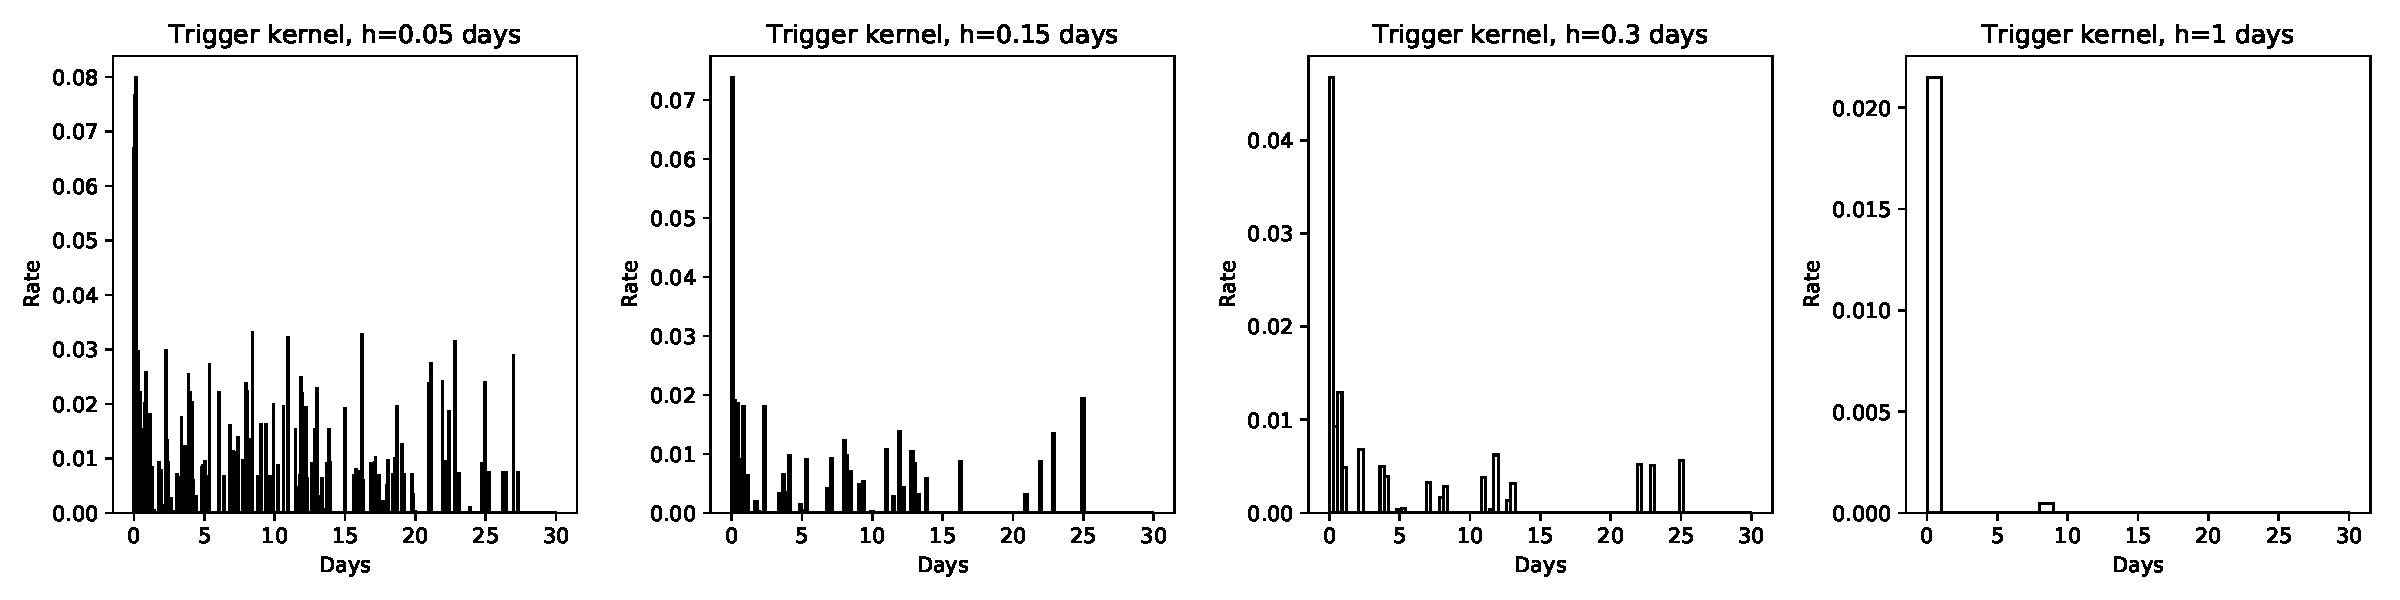
\includegraphics[width=\textwidth]{../notebooks/south_trigger.pdf}
  \caption{Histogram estimated trigger as the bandwidth varies.}
  \label{fig:south_trigger}
\end{figure*}

The results for the 2nd dataset are similar qualitatively, but differ in exact form.
In particular, with $h=0.3$ days, we get probability mass only a two isolated points
near 7 and 9 days; and with $h=1$ we get a much more pronounced spike at around 9 days.


\subsection{A kernel density estimator}\label{sec:grid_kde}

Having introduced the histogram estimator, we now look at using a full blown kernel density
estimator, see Appendix~\ref{app:grid_kde}.  In our analysis of the EM algorithm, we have
ignored ``edge correction issues'' as it seems computationally infeasible to do so.  However,
we typically have a large interval of data (say, a year) to fit the model to, and from the above
work, we expect that the trigger kernel will be shorted lived by comparison.

We initialise the model in the same way as in Section~\ref{sec:gbm}, so initially the trigger
kernel is exponential decay.  However, for all subsequent iterations of the EM algorithm,
we use a kernel density estimator.  Experiments suggest that the initial condition is not
terribly important, the end result of the iterative algorithm being the same.

When using a KDE method, we have to choose the bandwidth.  As \cite[Section~3.4]{sil} notes,
there is no completely satisfactory way of proceeding.  We can simply specify a bandwidth
up front.  There are various estimation procedures, from ``plug-in'' guesses (just looking
at the sample variance of the data, and the size of the data) to various cross validation
techniques.  As Silverman argues, cross validation can be difficult in the presence of
outliers or binned / discretised data.  A further complication for us is the unusual use of
variable ``weights'', which we see arising naturally from the EM algorithm,
Appendix~\ref{sec:his_est}.  It is far from clear how to adequately take account of these
weights in either cross-validation or even a ``plug-in'' estimate.

For the moment, we shall simply choose the bandwidth by hand, with a view to attempting to
learn something about the data.  Given a reproducible pattern, we might then try to find
a parametric form which captures it.  For completeness, we also follow the idea of \cite{sepp}
and use a variable bandwidth, the local bandwidth chosen by the distance to the $k$th nearest
neighbour, for various values of $k$.

We again use the South side of Chicago here.  The results are interesting, in that for small
bandwidths, we see temporally localised peaks in the trigger kernel, at 1, 2 and 4 days,
and then further peaks at 7, 8 and 11, 12 and 13 days.  As the bandwidth increases, these
are smoothed away until we get a curve which smoothly decays in time; see
Figure~\ref{fig:grid_kde_trigger}.  The nearest neighbour variable bandwidth pattern is
similar, Figure~\ref{fig:grid_kdenn_trigger}.  It is also worth noting that the estimated
value of $\theta$ decreases with increasing bandwidth, but stabilises for larger bandwidths.

\begin{figure*}
  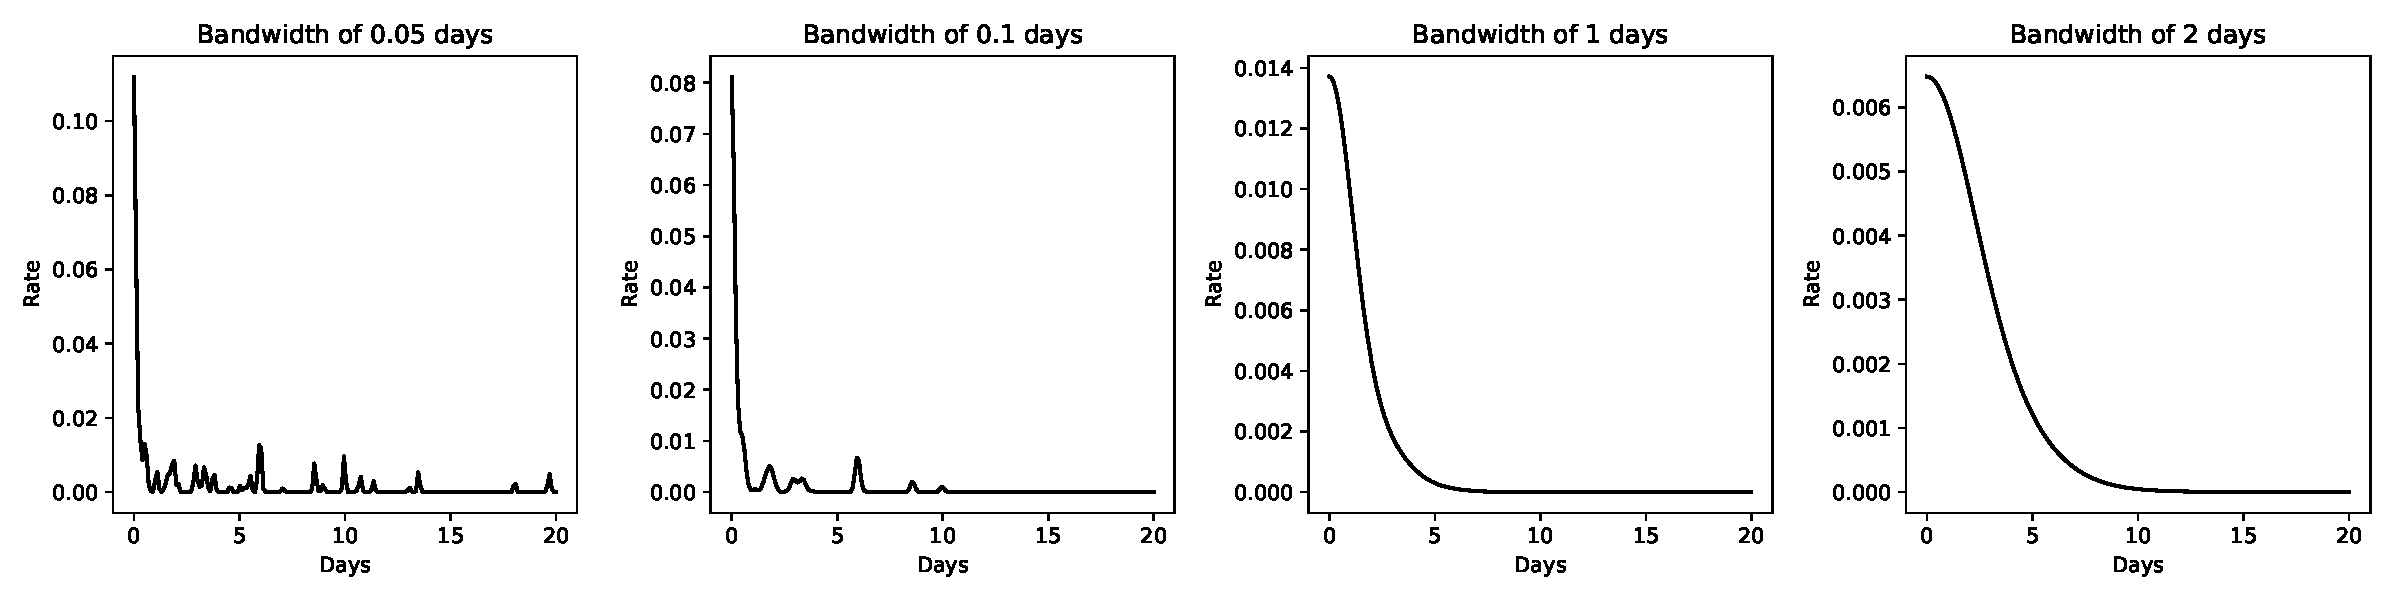
\includegraphics[width=\textwidth]{../notebooks/grid_kde_by_bandwidth.pdf}
  \caption{South side of Chicago, KDE estimated trigger kernels for differing bandwidths.}
  \label{fig:grid_kde_trigger}
\end{figure*}

\begin{figure*}
  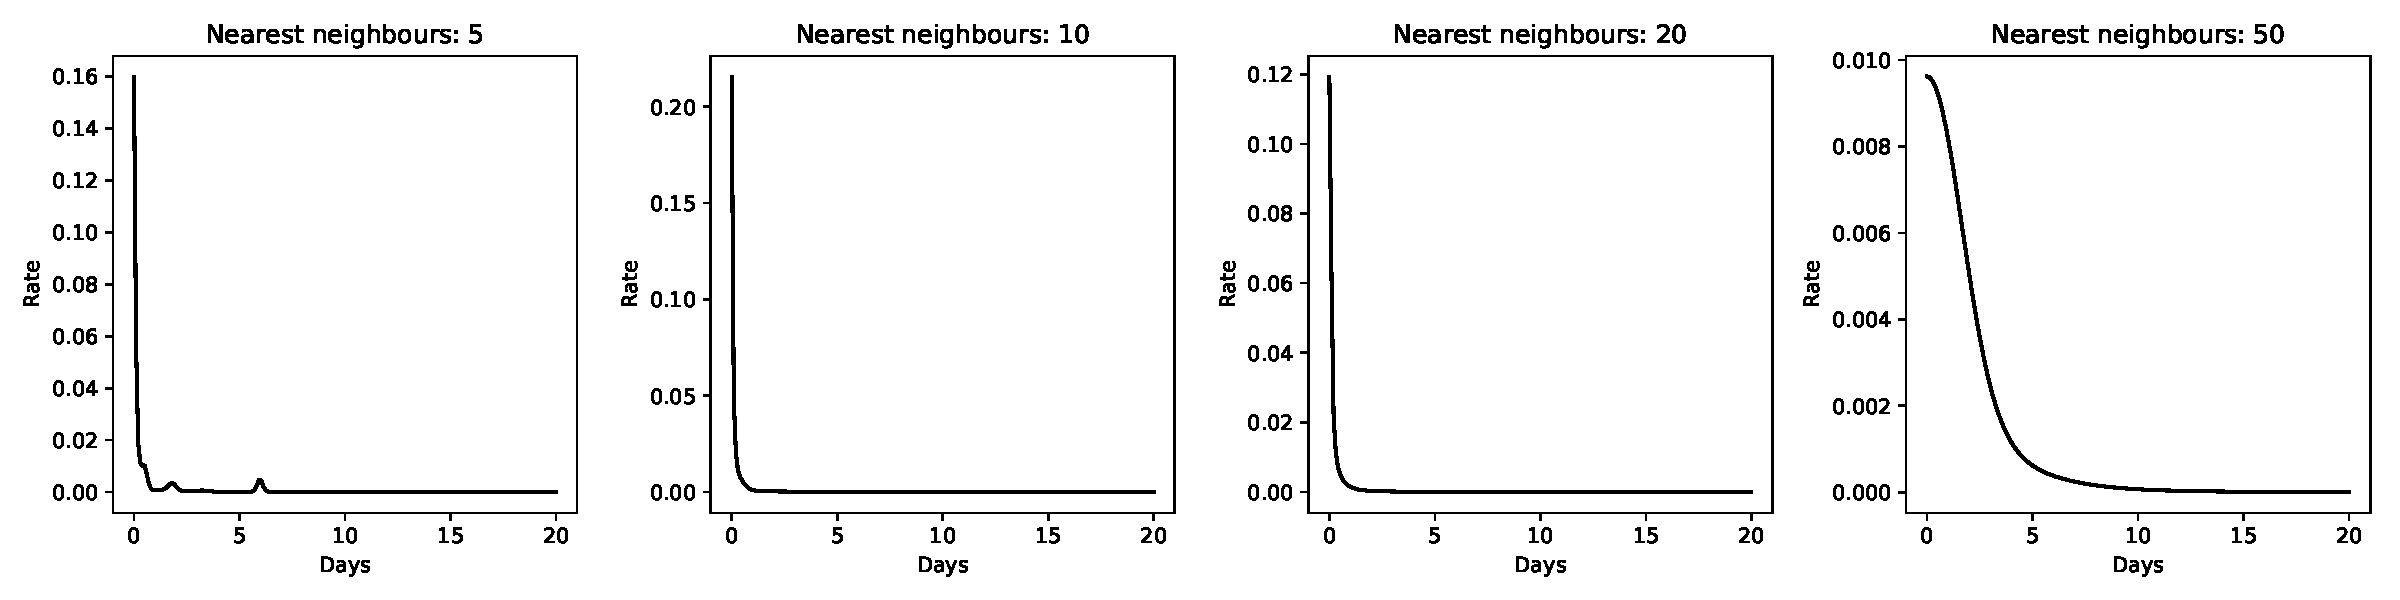
\includegraphics[width=\textwidth]{../notebooks/grid_kde_by_nn.pdf}
  \caption{South side of Chicago, KDE estimated trigger kernels for different nearest neighbour
  choices.}
  \label{fig:grid_kdenn_trigger}
\end{figure*}

With the second dataset, we get exactly the same results with a bandwidth of 1 or 2 days,
but slightly different kernels for smaller bandwidths; in particular, for $0.1$ days, we get
a big spike at 9 days.

We have also fitted this model to the simulated data we used in Figure~\ref{fig:sim_grid};
it does not perform terribly well, tending the estimate a trigger distribution with a much
longer tail than the real distribution, and being very noisy for smaller bandwidths.




\section{Allowing spatial interaction}\label{sec:grid_interact}

To move beyond this class of grid based model, we shall keep the grid ``histogram'' based
estimator of the background risk, but will consider the posibility of events from one grid
cell triggering events in another cell.  We will work with a very general triggering kernel,
but will assume that there is no link between space and time.  Thus the intensity is
\[ \lambda^*(t,x,y) = \mu_k + \sum_{t_i<t} \theta f(t-t_i) g(x-x_i, y-y_i), \]
where $k$ is the cell which $(x,y)$ falls in, but we now consider \emph{all} events before
time $t$, not just those in cell $k$.  Here $f$ governs the time triggering, and $g$ the
spatial triggering.

We showed previously that ``exact repeats'' in time can cause a maximum likelihood estimation of
parameters to estimate a parameter at $\infty$.  This will now also occur for exact repeats
in space, if $g$ is parameterised in such a way that it can approximate a delta function.
This is more troubling, as we expect exact repeats in space (because geocoding is likely
to assign the exact same coordinates to a building which is burgled twice) and because
artificial ``near repeats'' occur in our data: see the clustering we
observed in Figure~\ref{fig:chicago_overview}.  Notice that ignoring exact repeats in space
(by adjusting the $p$ matrix) seems unreasonable: we actually do want to model the exact repeats
we have just described.  It hence becomes critical to ensure that exact repeats do not
cause parameter estimates for $g$ to diverge.

We shall start with exponential decay in time, $f(t) = \omega e^{-\omega t}$ and a modified
Gaussian in space,
\[ g(x,y) = \begin{cases} \alpha &: x^2+y^2\leq r_0^2, \\
\beta e^{-(x^2+y^2)/2\sigma^2} &: x^2+y^2 > r_0^2. \end{cases} \]
So near the origin, $g$ is equal to $\alpha$, and further away is a Gaussian with shape
$\sigma$.  The parameter $r_0$ controls the change in behaviour, and will be chosen and fixed.
$\beta$ is a normalisation factor, see Appendix~\ref{app:grid_interact}.

The EM algorithm becomes a little more complicated here, for the details see
Appendix~\ref{app:grid_interact}.  The important thing to note is that in optimising the
trigger kernel, we now need to consider all order $N^2$ relations between the different
event times, as opposed to partly aggregating by grid cell.  Thus these algorithms take
longer to run.

A similar model was considered in \cite{mohler} (but a \emph{marked point process} in order
to model different crime types) where the background was estimated by a fixed bandwidth KDE
method.  The issue of exact repeats is discussed in this paper, and the offered solution is
to set $p_{i,j}=0$ if $t_i=t_j$ or the location of events $i$ and $j$ agree.  As argued above,
we find this unrealistic.

We performed a similar experiment to that which lead to Figure~\ref{fig:sim_grid}.  Here we
simulate background events as being distributed uniformly in each grid cell, according to
the background rate in that cell, and then simulate triggered events from the actual distribution
we are fitting to, but with $\alpha=0$.  The EM algorithm again fits well to this model.
We estimate the parameters fairly precisely, and the background rate is estimated well,
up to a similar error as we saw in Figure~\ref{fig:sim_grid}.

We fit the model to Chicago North Side data, again for the year 2016.  With an initial
experiment with $r_0=5m$ we estimate $\alpha\approx 8.19\times 10^{-3}, \sigma \approx 6.66$
and $\theta\approx 0.278$.  Thus there is certainly repeat-like behaviour, but it is very
tightly grouped in space (almost all the probability of the trigger kernel is within
20m of the triggering event, which seems unrealistically small).  The estimated value of
$\omega$ is now small, with $1/\omega \approx 153$ days!




\subsection{Interpreting fitted parameters}\label{sec:int_fit_params}

As we now have a completely spatial model, some care is required in interpreting values of
the intensity.  If we think back to equation (\ref{eq:exp_poisson}) then we see that if
we integrate $\lambda^*$ over a space-time region, we obtain a value which is the expected
number of events we'd observe in that region.  Suppose we care about the number of events
we'd see in a single grid cell in a single day, and let's suppose that the space trigger
component has support well contained in a grid cell (for this model, for real data, this
seems plausible).  Background events would contribute $\mu_k A$ events where $A$ is the
area of the grid cell, while an event which occurred $t$ time in the past, and close enough
to the grid to matter, would contribute around
\[ \theta \int_{t}^{t+1} f(t) \ dt = \theta e^{-\omega t} \big( 1 - e^{-\omega} \big) \]
extra events, on average.  However, to make sensible use of this information requires knowing
the distribution of past events.

As we are now seeing a trigger with a long tail, we have found it most useful to actually
form \emph{predictions} based upon the model.  This is explored more in
Section~\ref{sec:making_preds} below; but in the most simple form, it simply involves
evaluating the intensity function at a point in time, and different points in space.
How much the resulting risk surface differs from just the background rate gives a good
indication of how much the triggering is making a real difference, as applied to the actual data.

For the model we fitted, there is considerable variation in the resulting predictions,
both as the prediction time changes, and against the background rate.  We explore below whether
these predictions have much to say about reality.

Figure~\ref{fig:grid_vary_r0} shows how the estimated parameters vary as we change $r_0$.
Both $\theta$ and $1/\omega$ decrease rapidly once $r_0$ is greater than around 20m; this
is too small a value to be realistic, and the change is so sudden, that we conjecture that
it is caused by the artificial clustering
seen in the input data.  The dashed line in the plot for $\alpha$ is the ratio of $\alpha$ to
$\alpha_{\max}$.  When this is close to $1$, we are assigning almost no probability to the
gaussian decay part.  We see that $\sigma$ remains small, even for rather large $r_0$.

\begin{figure*}
  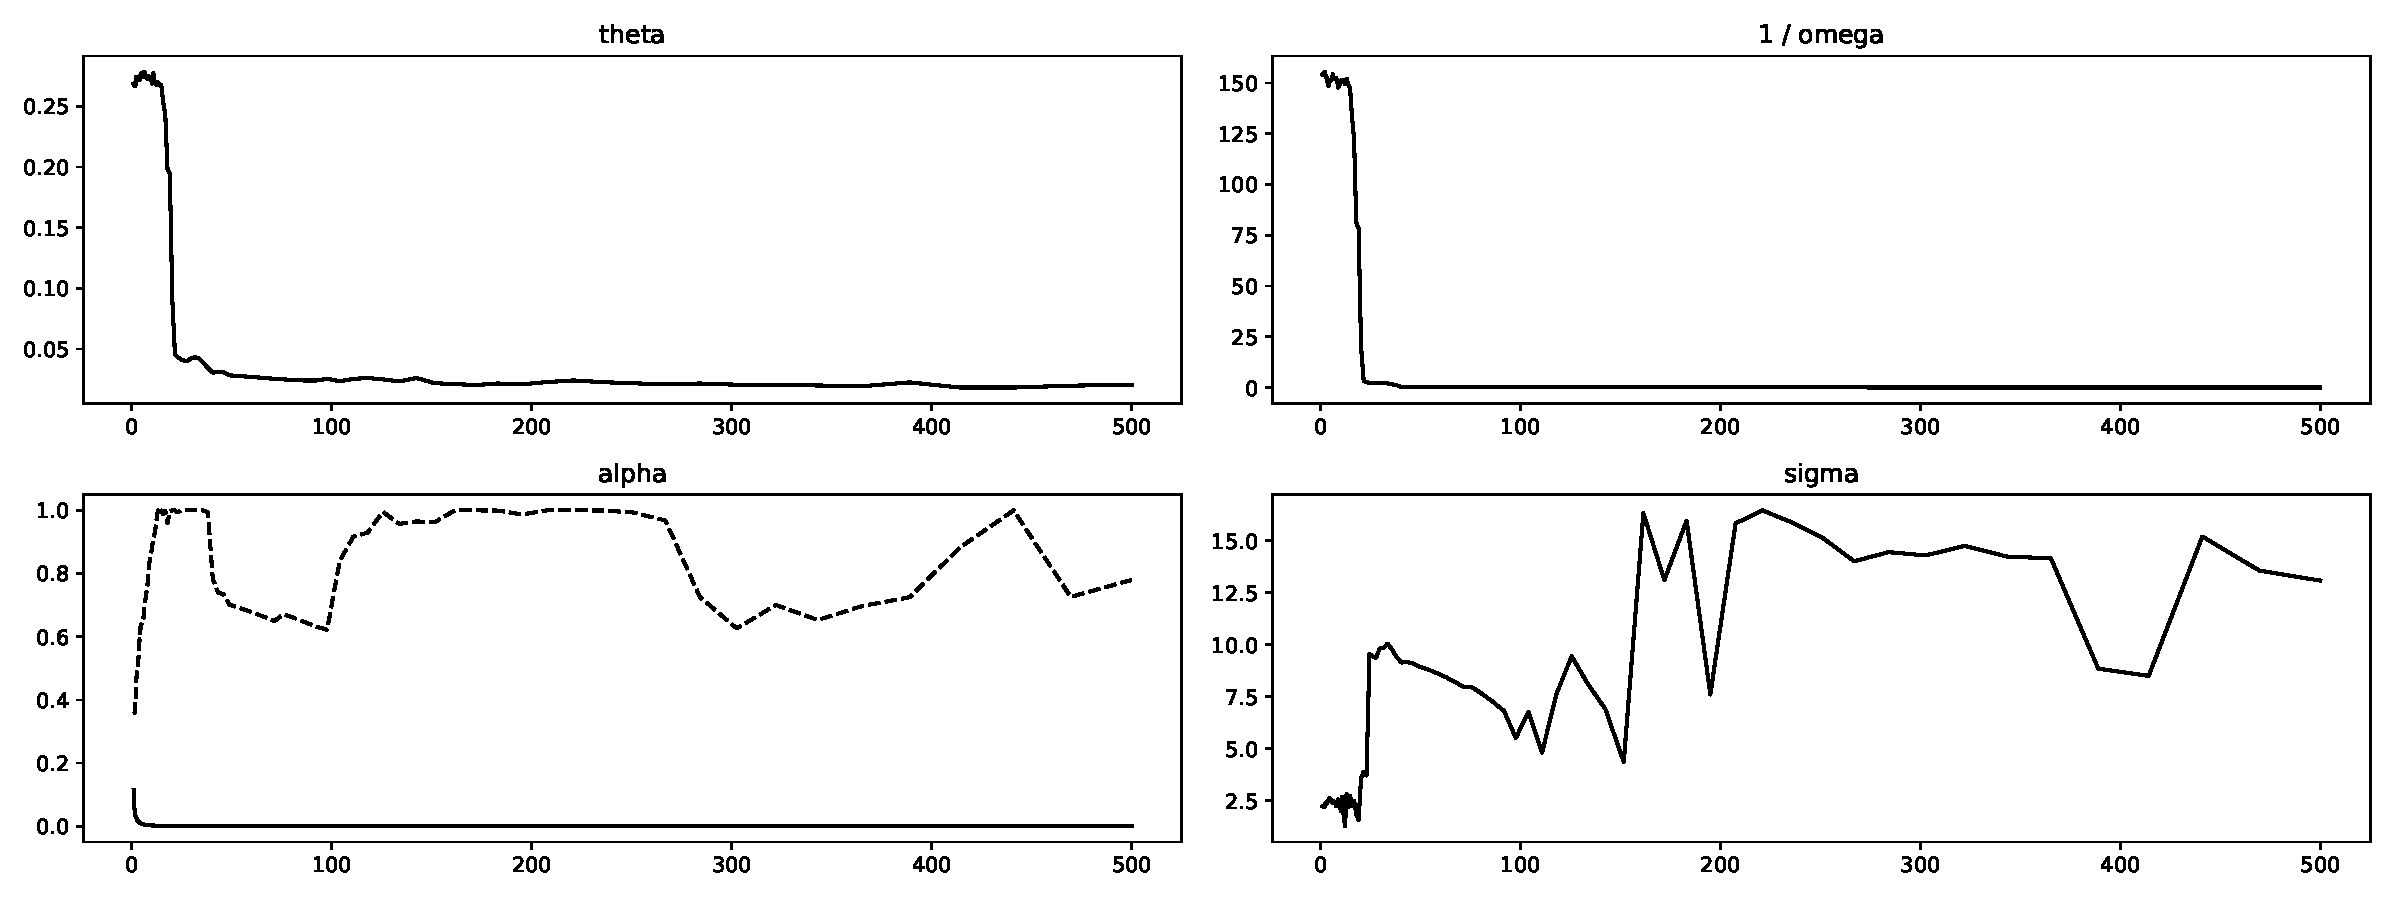
\includegraphics[width=\textwidth]{../notebooks/varying_r0.pdf}
  \caption{North side of Chicago, varying $r_0$ in the model described in Section~\ref{sec:grid_interact}.  For the plot for $\alpha$, in dashed, we plot $\alpha \pi r_0^2$
which is the total probability of the ``cap'' of $g$.}
  \label{fig:grid_vary_r0}
\end{figure*}

For the second dataset we see similar behaviour, but $\theta$ and $\omega^{-1}$ decay more
quickly.  (This removes evidence for the behaviour being caused by the artificial clustering.)
A qualitative difference is that $\alpha \pi r_0^2$ increases to 1 more slowly, between 0
and $r_0 = 200$m; similarly $\sigma\approx 10$m in this region.

In summary, we seem to actually gain rather little from the Gaussian decay term.  It is easy
to remove the Gaussian term, and simply let the triggering be uniform in a disc.  We then need
estimate only $\theta$ and $\omega$.  Figure~\ref{fig:grid_vary_r01} shows the result.  We see
the same cliff-edge like behaviour at around 20m.

\begin{figure*}
  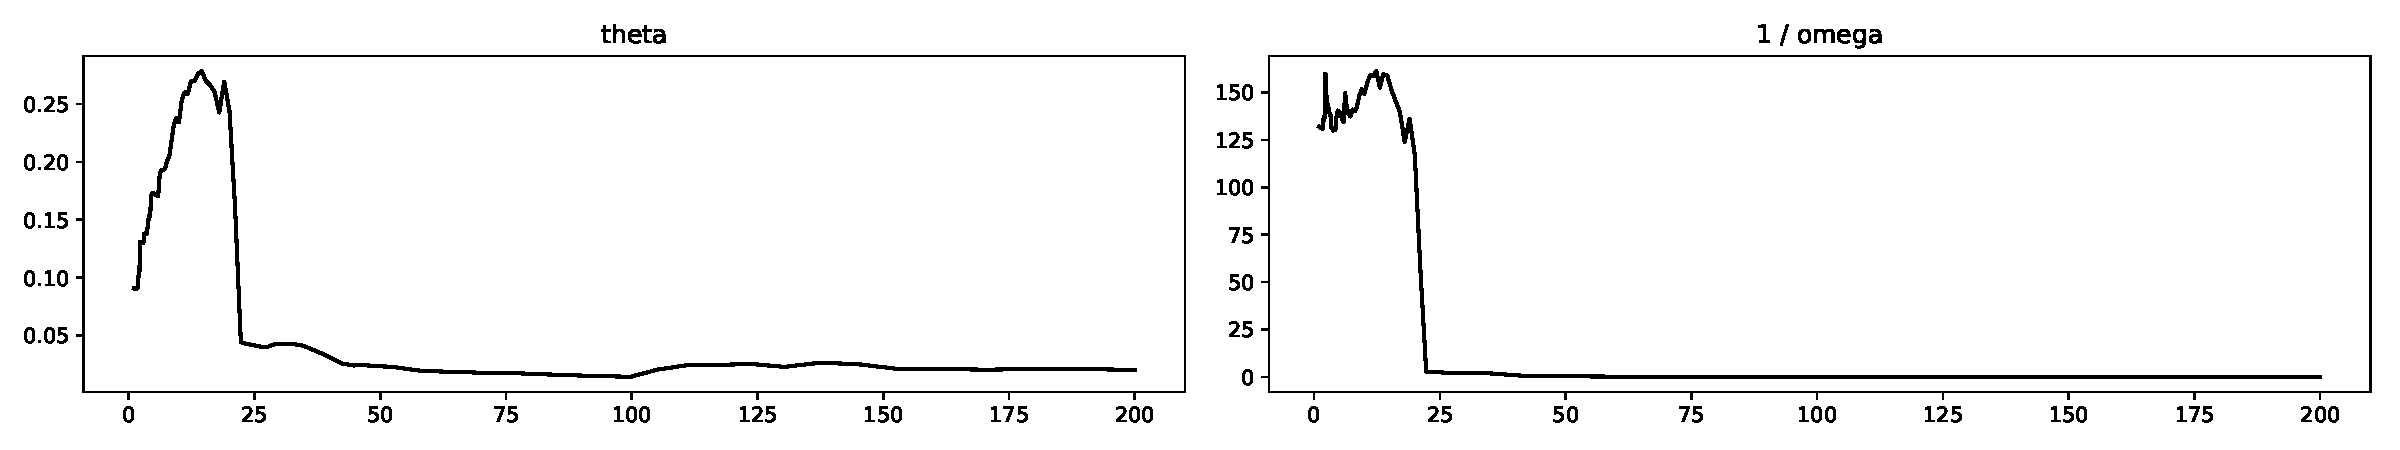
\includegraphics[width=\textwidth]{../notebooks/varying_r0_no_g.pdf}
  \caption{North side of Chicago, varying $r_0$ in the model described in Section~\ref{sec:grid_interact} without a Gaussian decay term.}
  \label{fig:grid_vary_r01}
\end{figure*}

For the second dataset, we see slightly different behaviour: $\omega^{-1}$ decays between
$r_0=0$ and $r_0=15$m, with a spike around $7$m.  $\theta$ behaves in a rather similar way,
and we do not see the increase and sudden cliff edge of Figure~\ref{fig:grid_vary_r01}.



\subsection{Histogram in time}

We implemented a histogram estimator for the time trigger $f$, using $g$ constant on a disc
of radius $r_0$, as before.  For small values of $r_0$, we get interesting repeat behaviour
from the histogram, but such behaviour seems very dependent on the bandwidth.  For larger
values of $r_0$, such at 100m or 250m (which seem realistic) we obtain repeat behaviour only
of the order of two days.  We note that, again, this model fits simulated data drawn from
the model well.  Technical details are in the short Appendix~\ref{app:grid_space_hist_time}.

For the second dataset, with our initial investigation with $r_0=20$m, we find that the overall
triggering risk is about 10 times smaller, regardless of the bandwidth used for the
histogram.  With $r_0=100m$ however we see rather similar trigger behaviour, with a longer
lasting trigger.  Similar behaviour occurs for $r_0=250m$.  This change is likely due to
the less ``clustered'' nature of the data, meaning that a large $r_0$ value leads to more
repeat behaviour being captured.




\subsection{KDE in time and space}\label{sec:kde_time_space}

It hence seems profitable to try to use a full KDE estimator for both $f$ and $g$.
We now run into computational challenges.  If we have $N$ points then we have order $N^2$
possible differences $t_j-t_i$ for $i<j$ (in the case of $f$),
and the KDE method requires forming a sum
over all these points, for each function evaluation.  As the next iteration of the EM algorithm
requires computing the $p$-matrix, order $N^2$ terms, we end up with an order $N^4$ algorithm.
This is too slow.  There are two possible speed-ups:
\begin{itemize}
\item We form a ``weighted'' KDE, with weights $p_{i,j}$.  If some of these numbers are
very small (or zero) they can be safely ignored with little (or no) impact on the estimated
function.
\item We might \emph{a priori} limit the support of $f$ and $g$ (e.g. to a few months and 500m,
or some similar values).  We could hence ignore $t_j - t_i$ larger than this value (and similarly
for $g$).  In practise, this could be achieved by setting the relevant $p_{i,j}$ value to $0$,
and then applying the previous idea.
\end{itemize}

We implement an adaptive, data-driven approach which combines these ideas.  For each column
of the $p$-matrix, we list the entries in decreasing order, and form the cumulative sum.  Any
entry which is beyond a cutoff (we use 99.9\%) we set to 0.  We then form the KDEs, but use the
input data to estimate the support.  This gives an automatic algorithm which leads to considerable
speedup.  However, the resulting algorithm is still very slow (e.g. on large simulated datasets).
On the Chicago dataset it is slow, but acceptable; the first issue above appears to be the
critical one as far as speed is concerned.

The basis of the EM algorithm is to introduce ``hidden variables'' which simplify the likelihood
calculation, and then to iterate taking the expectation over the hidden variables, and then
maximising the parameters.  As is common in computational statistics, if we cannot compute the
expectation, then it may be possible to \emph{sample} from the distribution at hand.  This leads
to the ``monte carlo E-step'', see \cite[Chapter~6]{mk}.  An extreme form of this is to take one
sample from the distribution of the hidden variables, the ``stochastic EM algorithm''.  In our
setting, this corresponds to, at each iteration, using the $p$-matrix to take a sample of which
events are ``background'', and which are ``triggered''.  We then use these identified events
to maximise our parameters, and/or form a KDE etc.  This is the approach taken in \cite{sepp2},
following \cite{zovj} (although they do not explicitly make connections with the EM algorithm).

This stochastic EM algorithm has the disadvantage of not using all the information we have about
the branching process: we assign each point as either background or triggered, even if the
current $p$-matrix suggests that both are equally likely.  However, a large advantage is that
we simplify and speed up the KDE, especially for the triggering, as we will now only have order
$N$ points to consider, instead of $N^2$.  However, as we shall shortly see, on real data,
the stochastic EM algorithm can lead to different (and, frankly, incorrect) results, as compared
to the ``full'' EM algorithm.

We fit simulation data (drawn from the same distribution as the model) and obtain a good match.
As observed in previous studies (see \cite{sepp2} or \cite[Figure~3]{rc}) the time component of
the trigger tends to underestimate near $0$.  This is because the Gaussian based KDE method,
even with reflection about $t=0$, does not well capture the exponential decay which we use
in the simulation.  Both the full EM algorithm and the stochastic variant perform equally well.

We observe some very interesting behaviour from real data.  Figure~\ref{fig:grid_kde_1} shows
an initial result, with $f$ estimated with a bandwidth of 1 day, and $g$ estimated with a bandwidth
of 10 metres.  We obtain $\theta=0.34$.  The vertical lines in the plot of $f$ indicate each day;
for example, we see a peak somewhere between 21 and 22~days.
The estimate for $g$ involves very small numbers, so to better visualise, we have shown the
surface for $\log(e^{-20}+g)$.

As argued in Section~\ref{sec:int_fit_params}, it can be very hard
to interpret these plots, except in general terms.  One possible visualisation technique is motivated
by the stochastic EM algorithm: we can use the fitted model to form a $p$-matrix, and then take
a sample of which events are background, and which are triggered.  Figure~\ref{fig:grid_kde_1a}
shows the result: we plot both the trigger ``delta'' (the vector $(t_j-t_i, x_j-x_i, y_j-y_i)$)
and a (plug-in bandwidth) KDE, using the same visualisation strategy of plotting $\log(\epsilon+k)$
for some small $\epsilon$, to visualise the density.  In both the plot of $g$, and the sample,
we see a clear grid like pattern.  This is a reflection of the north/south and east/west grid
layout of streets in Chicago, together we the observed ``clustering'' from
Figure~\ref{fig:chicago_overview}.  That we see such a pronounced grid pattern should not surprise
us, given the geography of Chicago, but whether the artifical clustering in the input data
exaggerates this is unknown.

We note that if we continue to run the EM algorithm for further iterations (which is time
consuming!) then the shape of the triggers does not qualitatively change, but $\theta$ (the
overall trigger risk) does tend to increase; after 200 iterations we have $\theta=0.44$.

With the second dataset, Figure~\ref{fig:grid_kde_1_mod},
we get a smaller value for $\theta$, namely $0.17$, and a rather different
behaviour for the time trigger, with nearly linear decay on the order of 8 or 9 days.  The space
trigger does look similar, suggesting the ``grid'' pattern we observe here is due to the geography
of Chicago, and not just the artificial clustering in the initial input data.
A plot of the estimated trigger points, not shown, is similar to Figure~\ref{fig:grid_kde_1a}
but shows less ``clumpy-ness'' in space.  If we run the EM algorithm for further iterations,
then again $\theta$ increases (to $0.26$ after 200 iterations) and the time trigger develops a
noticeable bump at 4 days.

\begin{figure*}
  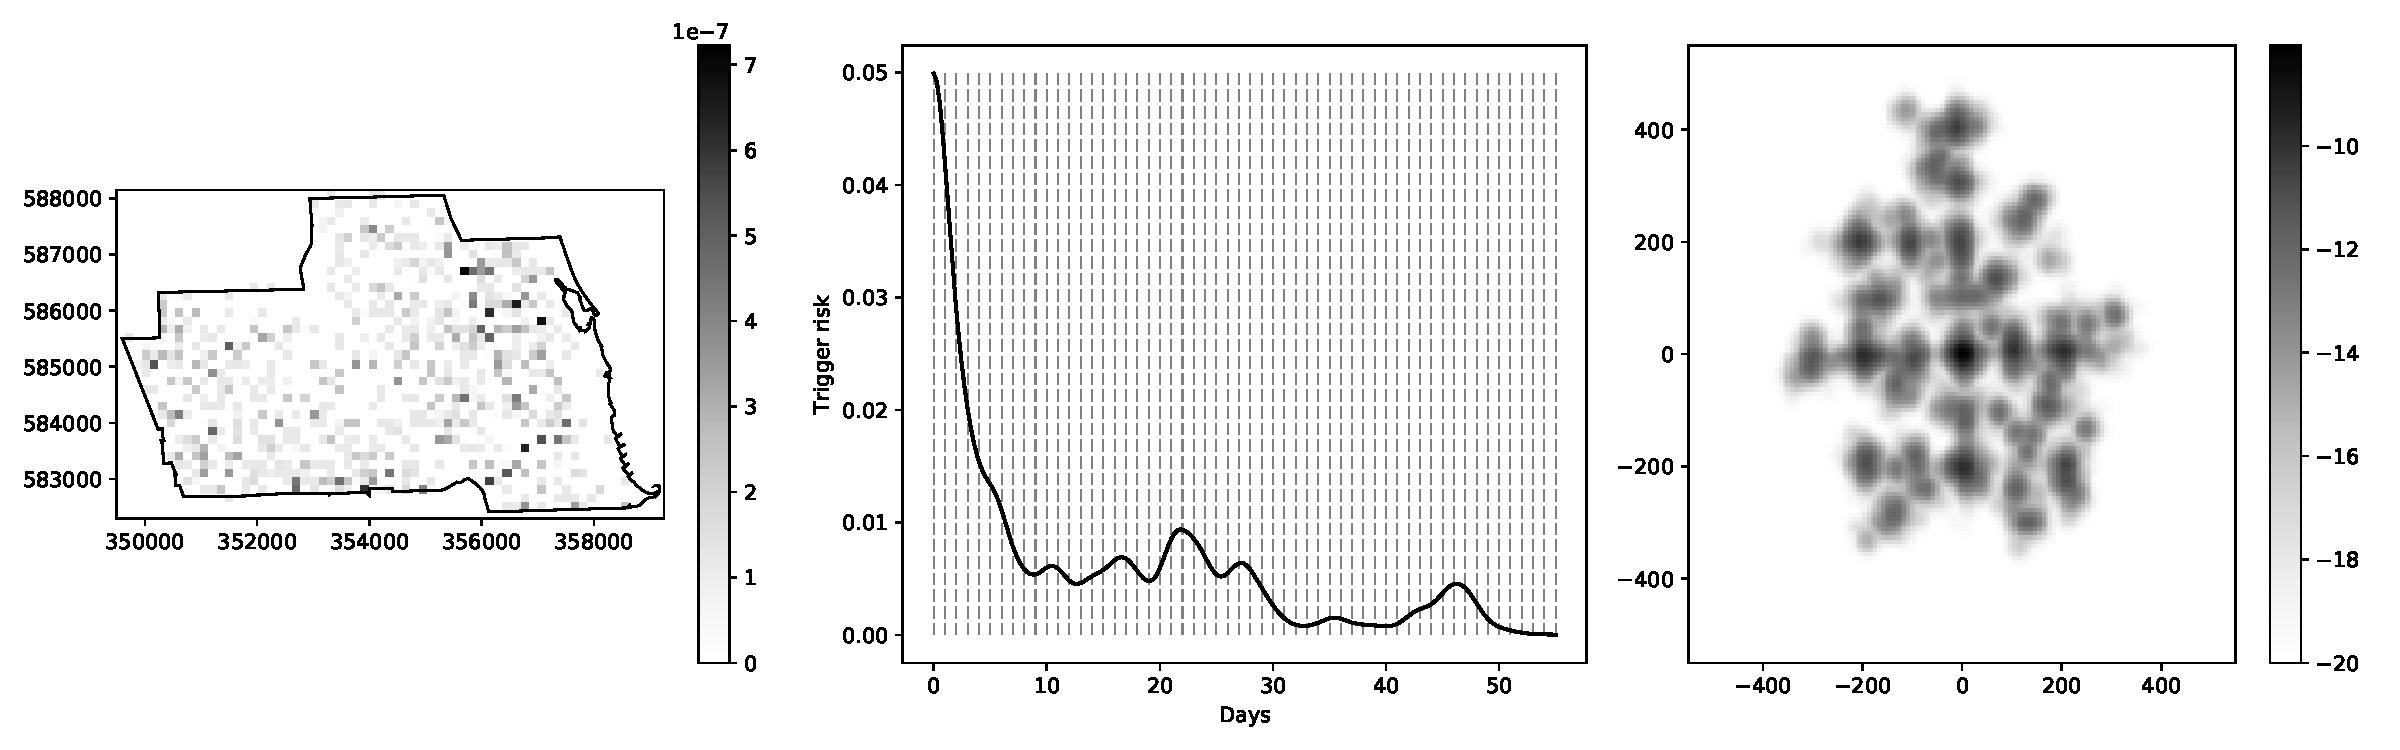
\includegraphics[width=\textwidth]{../notebooks/grid_kde_one.pdf}
  \caption{North side of Chicago, for the model described in Section~\ref{sec:kde_time_space},
  with a time bandwidth of 1 day, and a space bandwidth of 10 metres.  From left to right we show
  the background rate, the time kernel $f$, and the space kernel $g$.  For $g$ we actually plot
  the surface $\log(e^{-20}+g)$.}
  \label{fig:grid_kde_1}
\end{figure*}

\begin{figure*}
  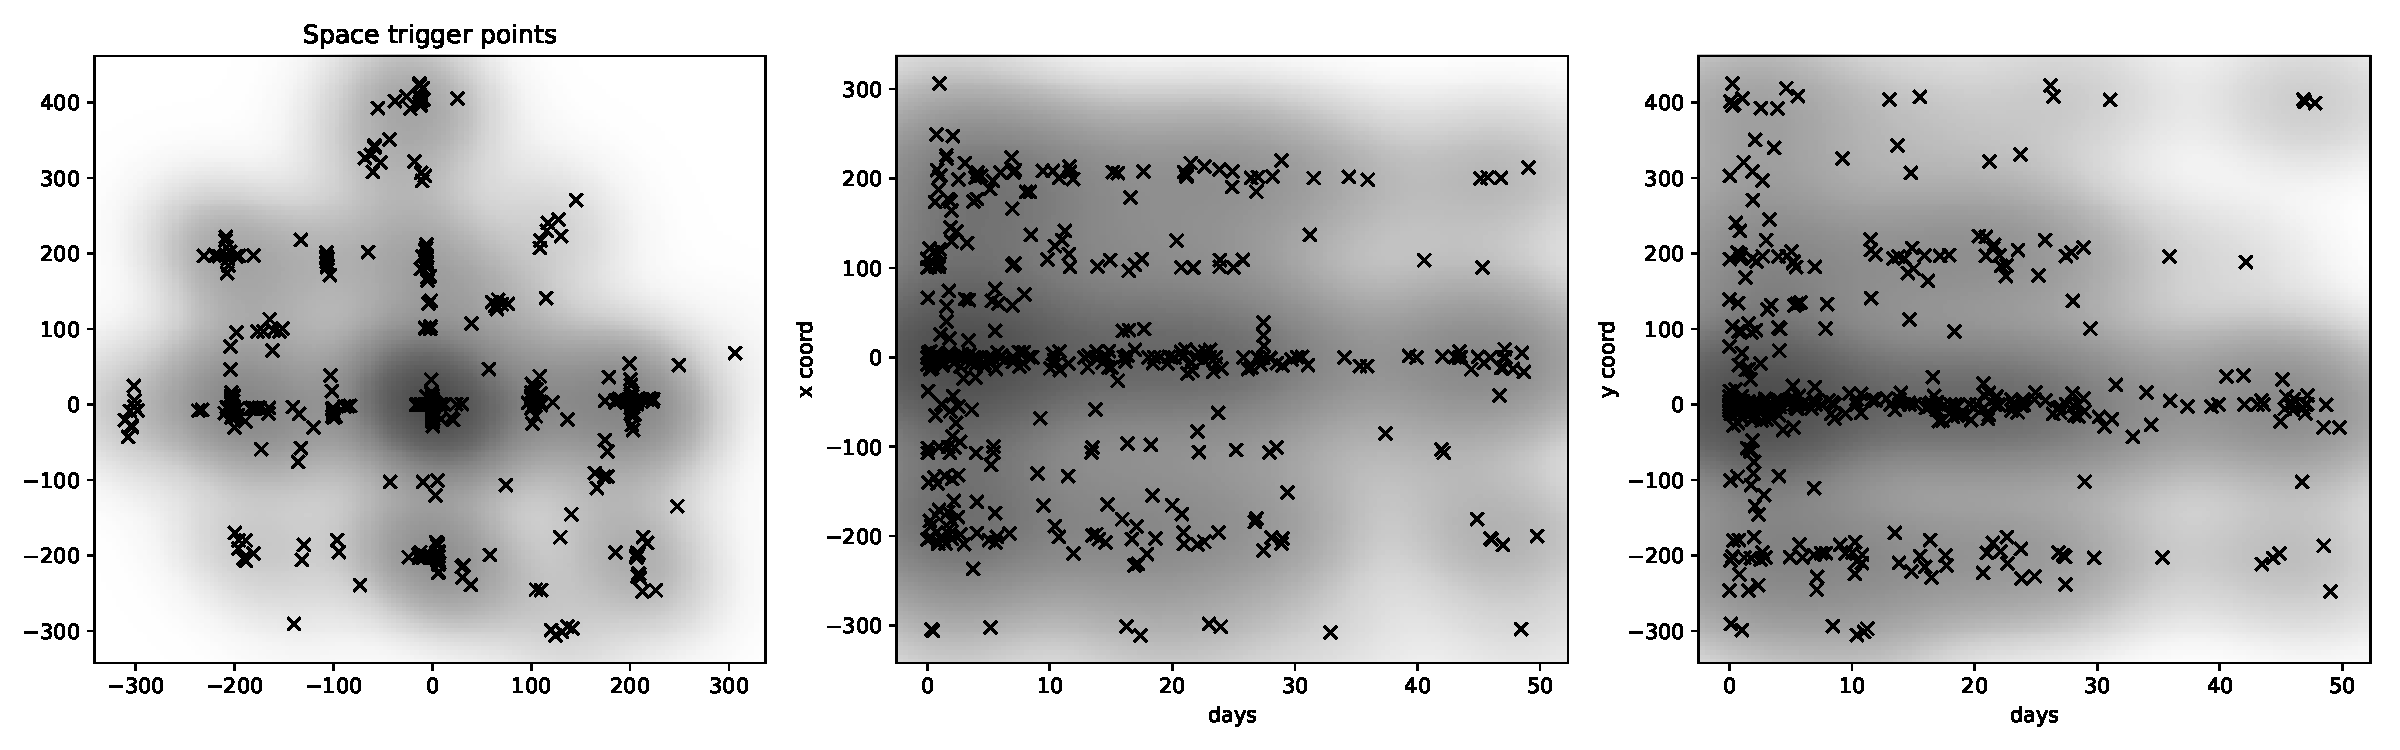
\includegraphics[width=\textwidth]{../notebooks/grid_kde_onea.pdf}
  \caption{For the model from Figure~\ref{fig:grid_kde_1}, sampled trigger points.}
  \label{fig:grid_kde_1a}
\end{figure*}

\begin{figure*}
  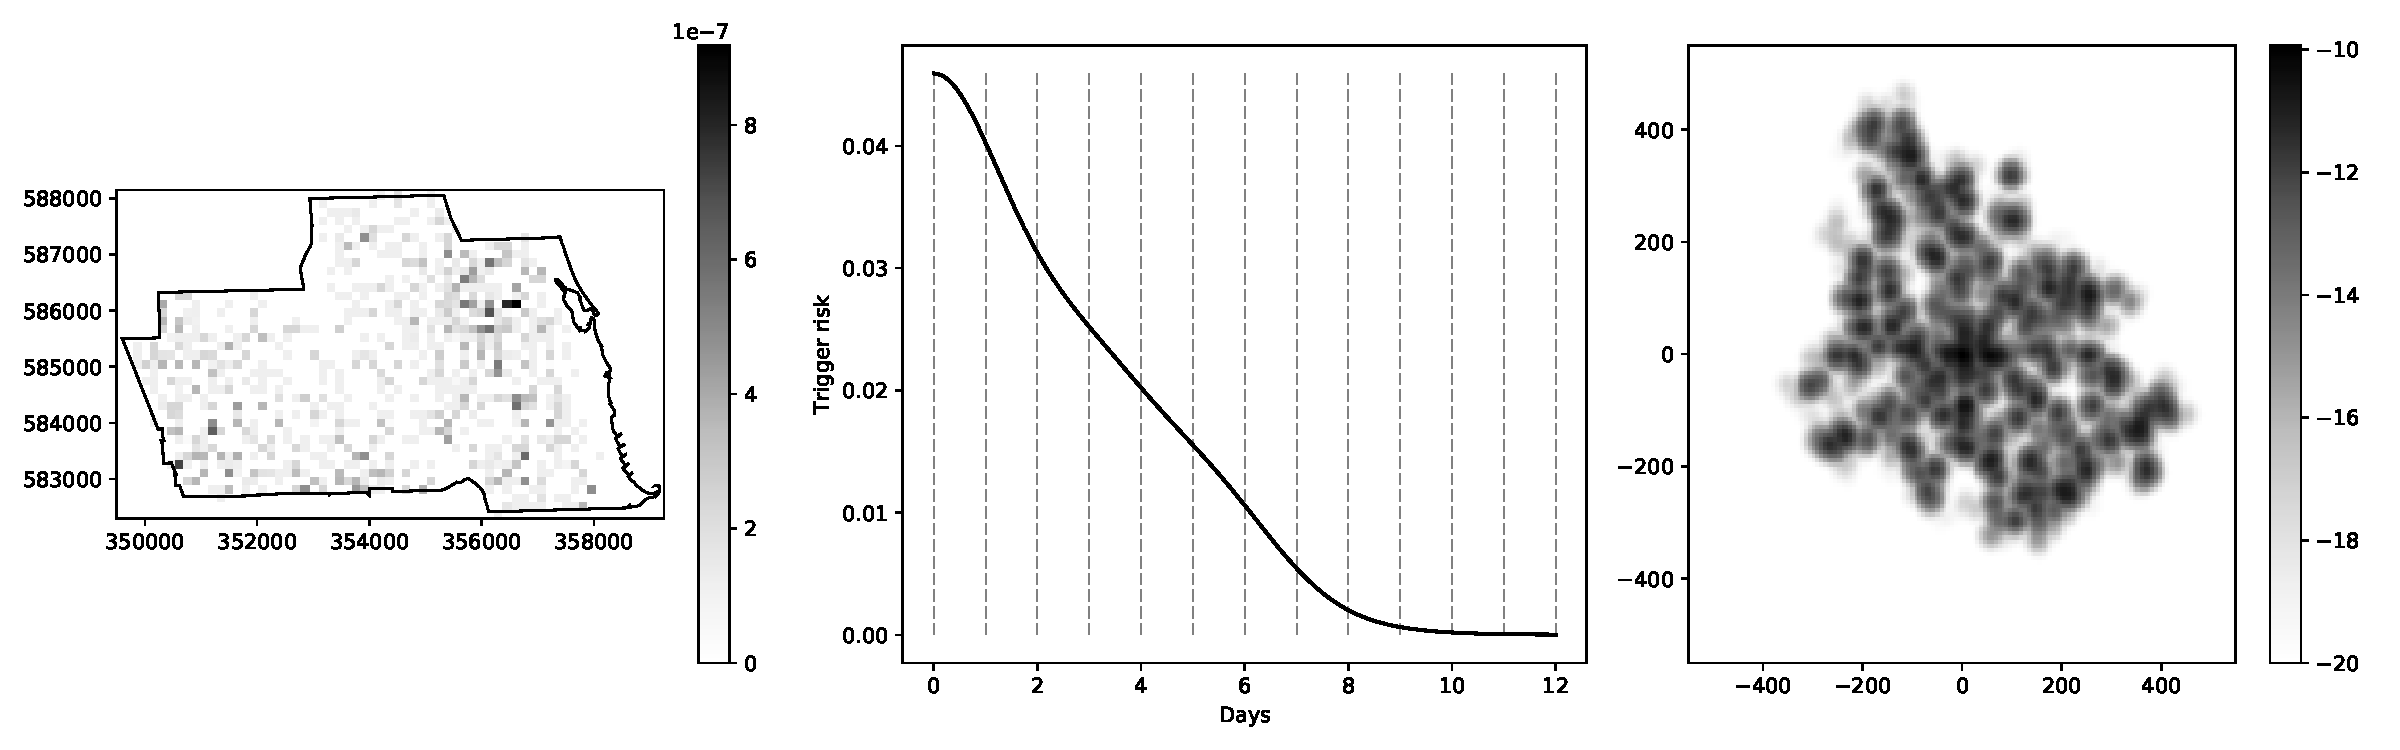
\includegraphics[width=\textwidth]{../notebooks/grid_kde_one_mod.pdf}
  \caption{As Figure~\ref{fig:grid_kde_1} but with the second dataset.}
  \label{fig:grid_kde_1_mod}
\end{figure*}

We fitted the same model using the stochastic EM algorithm, and obtained quite different results,
see Figure~\ref{fig:grid_kde_2} (the sample of trigger points plot is similarly different).
The estimated value of $\theta$ is $0.16$, about half that we saw before.  The time kernel is
similar is shape, but with different quantitative properties.  The space kernel is also similar
in shape, but with a much smaller support, and is much less symmetric.
We believe that these differences are caused by
exactly the problem we identified above, namely that by sampling, we assign for definite that
each point is either background or triggered, instead of allowing a mixture.  Taking the full
expectation allows us to take account of the probability that an event is triggered, and hence
allow that event to contribute some weight to the KDE.  The second dataset exhibits
similar behaviour: again $\theta$ is smaller, at $0.053$, the time trigger is similar, but
the space trigger is much more localised in space.

\begin{figure*}
  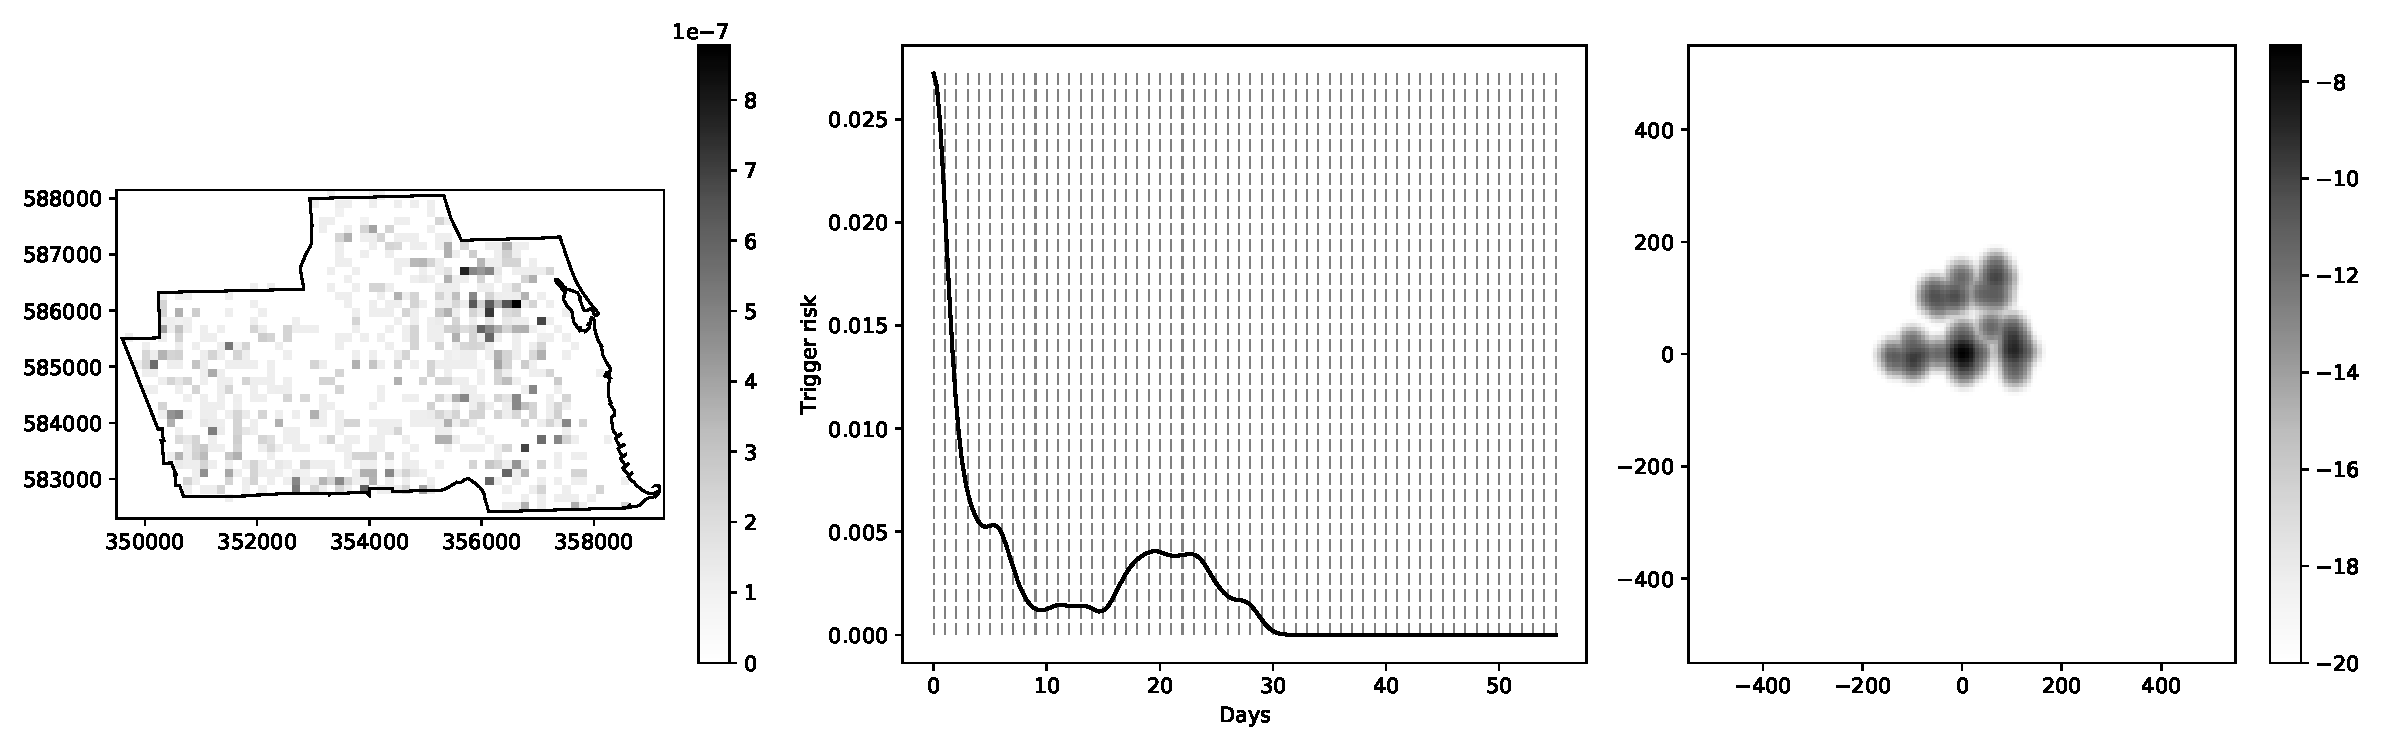
\includegraphics[width=\textwidth]{../notebooks/grid_kde_two.pdf}
  \caption{North side of Chicago, as in Figure~\ref{fig:grid_kde_1}, but model fitted using the
  stochastic EM algorithm.}
  \label{fig:grid_kde_2}
\end{figure*}

Unfortunately, these results seem to (yet again) depend a great deal on the bandwidths chosen.
Figure~\ref{fig:grid_kde_3} shows the same model as Figure~\ref{fig:grid_kde_1} but now $g$ uses
a bandwidth of 50 metres.  The resulting estimate for $g$ is much smoother (of course), but also
$\theta$ becomes $0.058$ while the $f$ now smoothly and quickly decays in the order of a week.
With our second dataset, we get $\theta=0.036$ but rather similar kernel shapes.  By adjusting
the bandwidths, we obtain a rather wide range of behaviours.

\begin{figure*}
  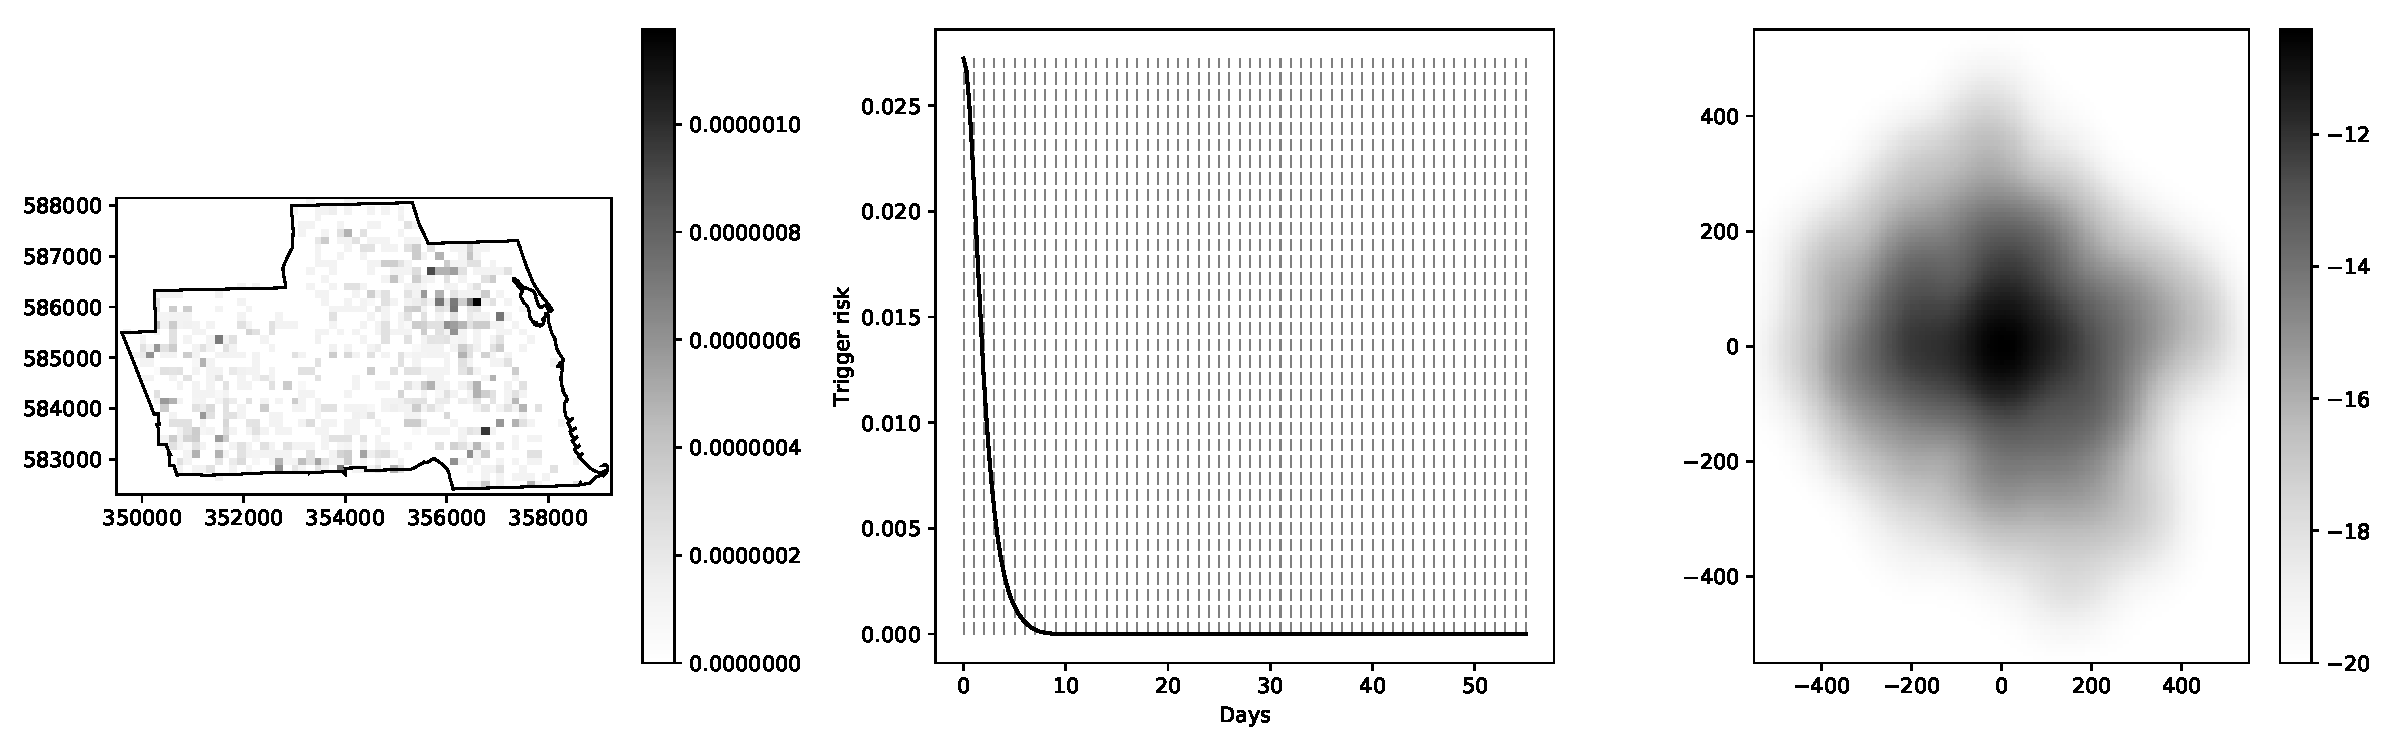
\includegraphics[width=\textwidth]{../notebooks/grid_kde_three.pdf}
  \caption{North side of Chicago, for the model described in Section~\ref{sec:kde_time_space},
  with a time bandwidth of 1 day, and a space bandwidth of 50 metres.}
  \label{fig:grid_kde_3}
\end{figure*}

The authors of \cite{sepp} and \cite{zovj} suggest using a variable bandwidth KDE with the
bandwidth for each point chosen by the distance to the $k$th nearest neighbour; \cite{sepp}
uses a value of $k=15$.  We use the same idea for the space kernel $g$, keeping the time
kernel as being a fixed bandwidth of 1 day.  The results are shown in Figure~\ref{fig:grid_kde_4};
here $\theta = 0.38$.  Of note is the very long fall-off in time, and the large support for the 
space kernel $g$.  We artificially forced the support of $g$ to be within a disk of radius 1500m,
to speed up the algorithm (which is still extremely slow).  Notice that the support of $g$
really does extend to the edge of this disk, and that it has a strong pattern.  The sampled
trigger points, Figure~\ref{fig:grid_kde_4a}, similarly shows a very strong pattern; notice
that the spatial extent is somewhat larger than that seen in Figure~\ref{fig:grid_kde_1a},
though the pattern is rather similar.

\begin{figure*}
  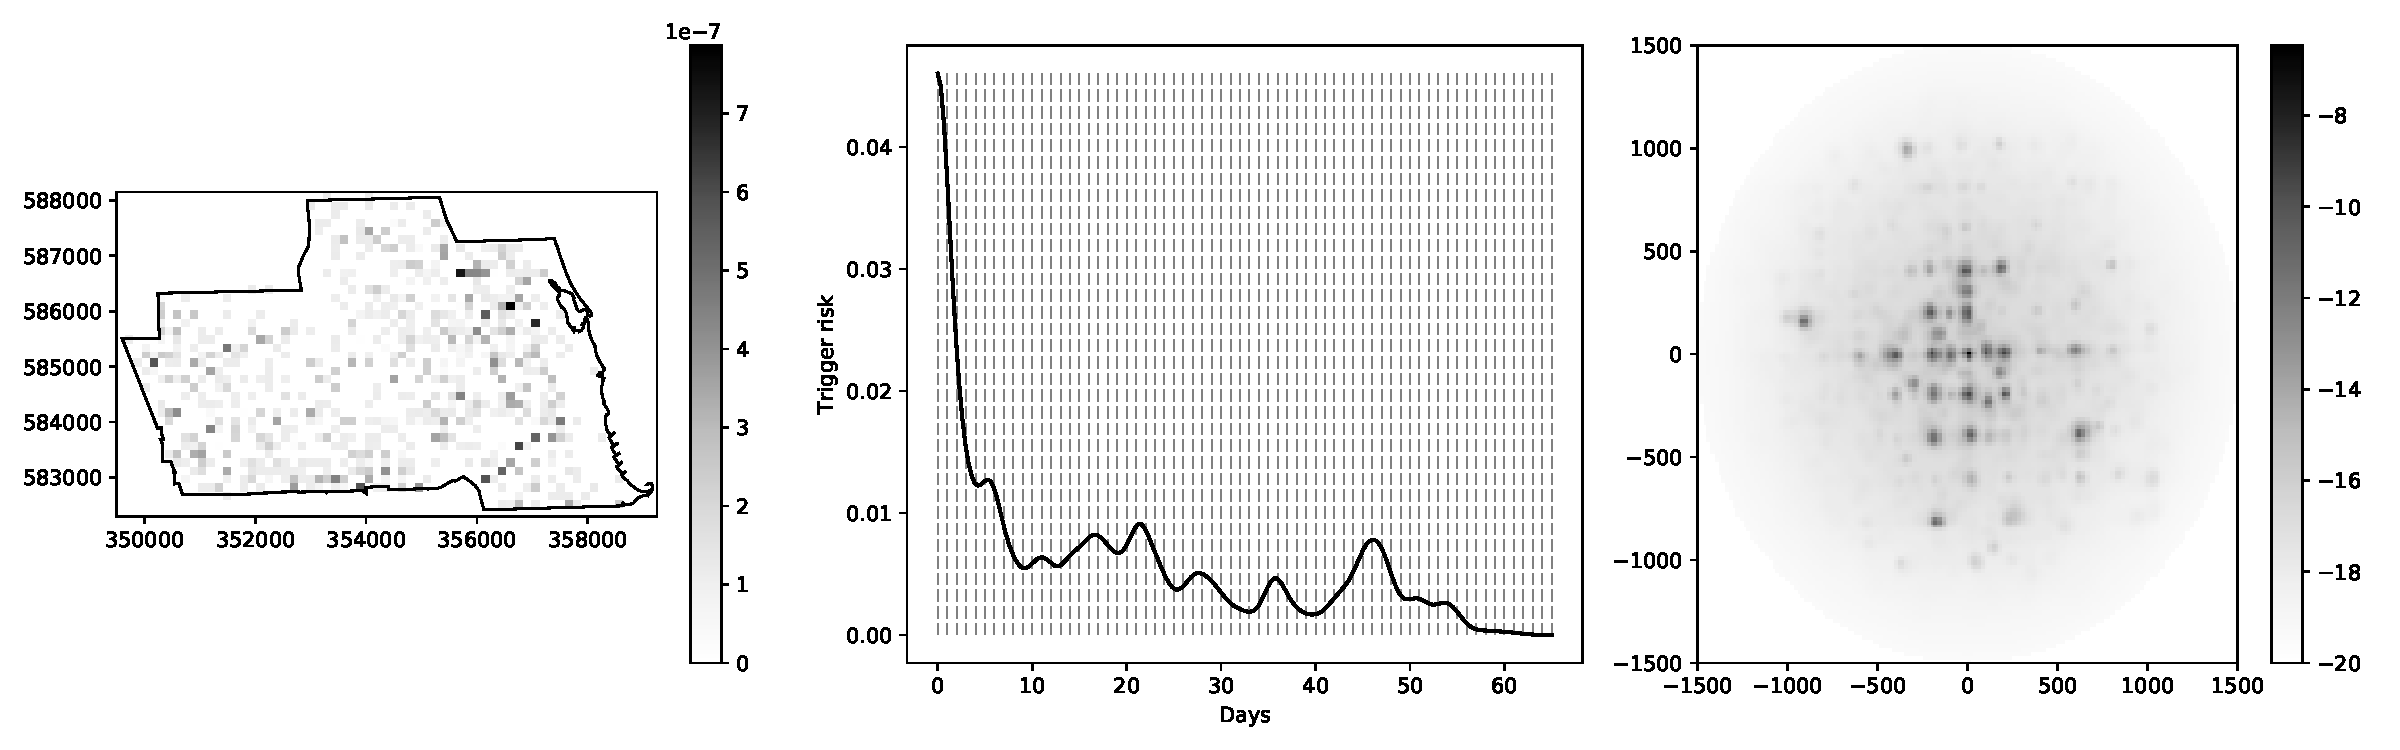
\includegraphics[width=\textwidth]{../notebooks/grid_kde_knn1.pdf}
  \caption{North side of Chicago, for the model described in Section~\ref{sec:kde_time_space},
  with a time bandwidth of 1 day, and the space kernel estimated with a nearest neighbour variable
  bandwidth, $k=15$.}
  \label{fig:grid_kde_4}
\end{figure*}

\begin{figure*}
  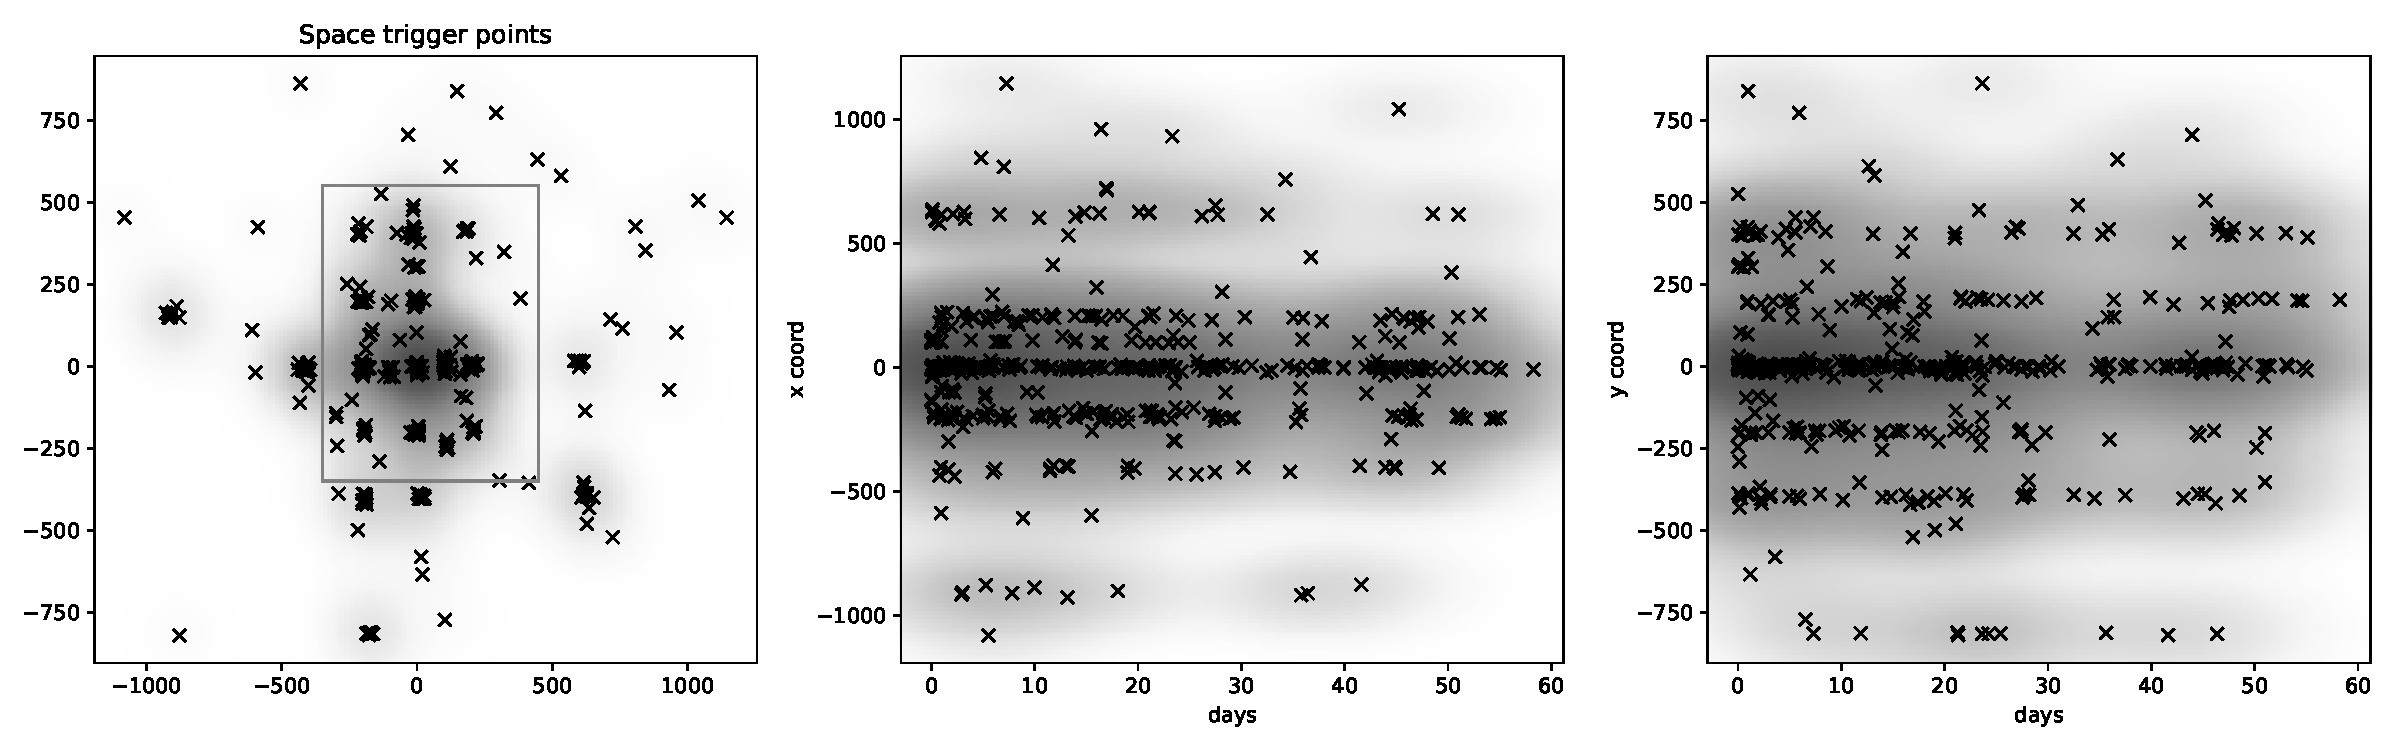
\includegraphics[width=\textwidth]{../notebooks/grid_kde_knn2.pdf}
  \caption{Sampled trigger points from the model fitted as in Figure~\ref{fig:grid_kde_4}.
  In the left plot, outlined is the region we show in the corresponding plot of
  Figure~\ref{fig:grid_kde_1a}.}
  \label{fig:grid_kde_4a}
\end{figure*}

Again such behaviour seems hugely dependent on the chosen bandwidth.  By varying the
value of $k$, or the fixed bandwidth used for $f$, we observe a large range of different behaviours
and, especially, a large range in the value of $\theta$.

Furthermore, and of particular interest given the algorithm used in \cite{sepp}, we ran the same
model as lead to Figure~\ref{fig:grid_kde_4}, but using the stochastic EM algorithm.  The speed of
execution is far quicker, but the result, Figure~\ref{fig:grid_kde_5}, is radically different, with
a huge east/west bias in the triggering kernel.  The sampled trigger points (not shown) show a similar
bias.  It is extremely interesting that a similiar ``bias'' was found in \cite{rc}; there, the
authors proposed the solution of enforcing radial symmetry on the triggering kernel.  Our results
here suggest that the bias is actually caused by using the approximation of the stochastic EM
algorithm instead of the ``full'' EM algorithm.

\begin{figure*}
  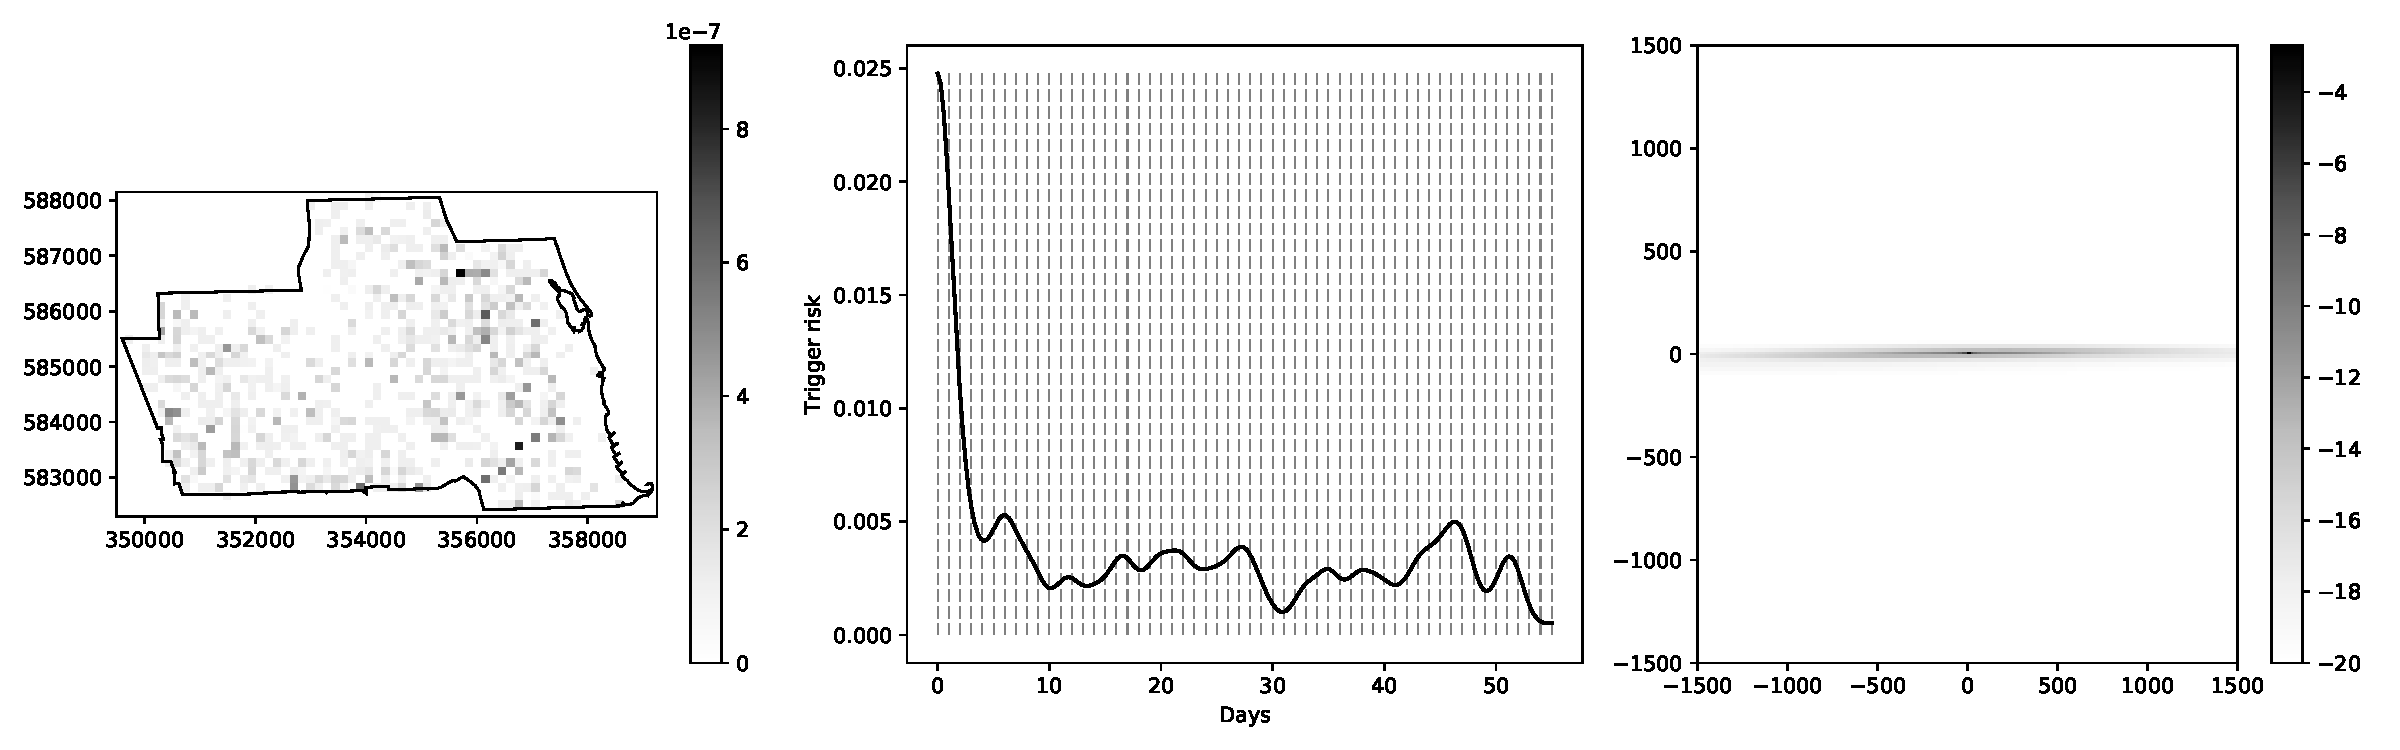
\includegraphics[width=\textwidth]{../notebooks/grid_kde_knn_sem_1.pdf}
  \caption{North side of Chicago, for the model described in Section~\ref{sec:kde_time_space},
  with a time bandwidth of 1 day, and the space kernel estimated with a nearest neighbour variable
  bandwidth, $k=15$.  Uses the stochastic EM algorithm.}
  \label{fig:grid_kde_5}
\end{figure*}

We cannot present the same findings for the second dataset because the stochastic EM algorithm
refuses to run for many iterations before stopping with numerical errors.  This occurs because
the sampled number of triggered points becomes too small.




\subsection{Joint dependance in trigger}\label{sec:joint_grid}

Instead of supposing that the trigger density factorises as $f(t)g(x,y)$ we can instead use a KDE
to estimate the joint time/space density.  This approach is close in spirit to \cite{sepp}.
As time and space have different dimensions, we first scale the $x$ and $y$ coordinates by a factor
of 20, and then treat the data as being three dimensional, with a bandwidth of 1.
Figure~\ref{fig:full_kde_1} shows the result, showing marginal distributions (that is, integrate
out the other variables).  For the marginal time kernel, we fit an exponential (dashed line)
which shows very good agreement.  The marginal space kernel is visualised in the same way as
before (plot $\log(e^{-20}+g)$) and shows the by now familiar pattern.

\begin{figure*}
  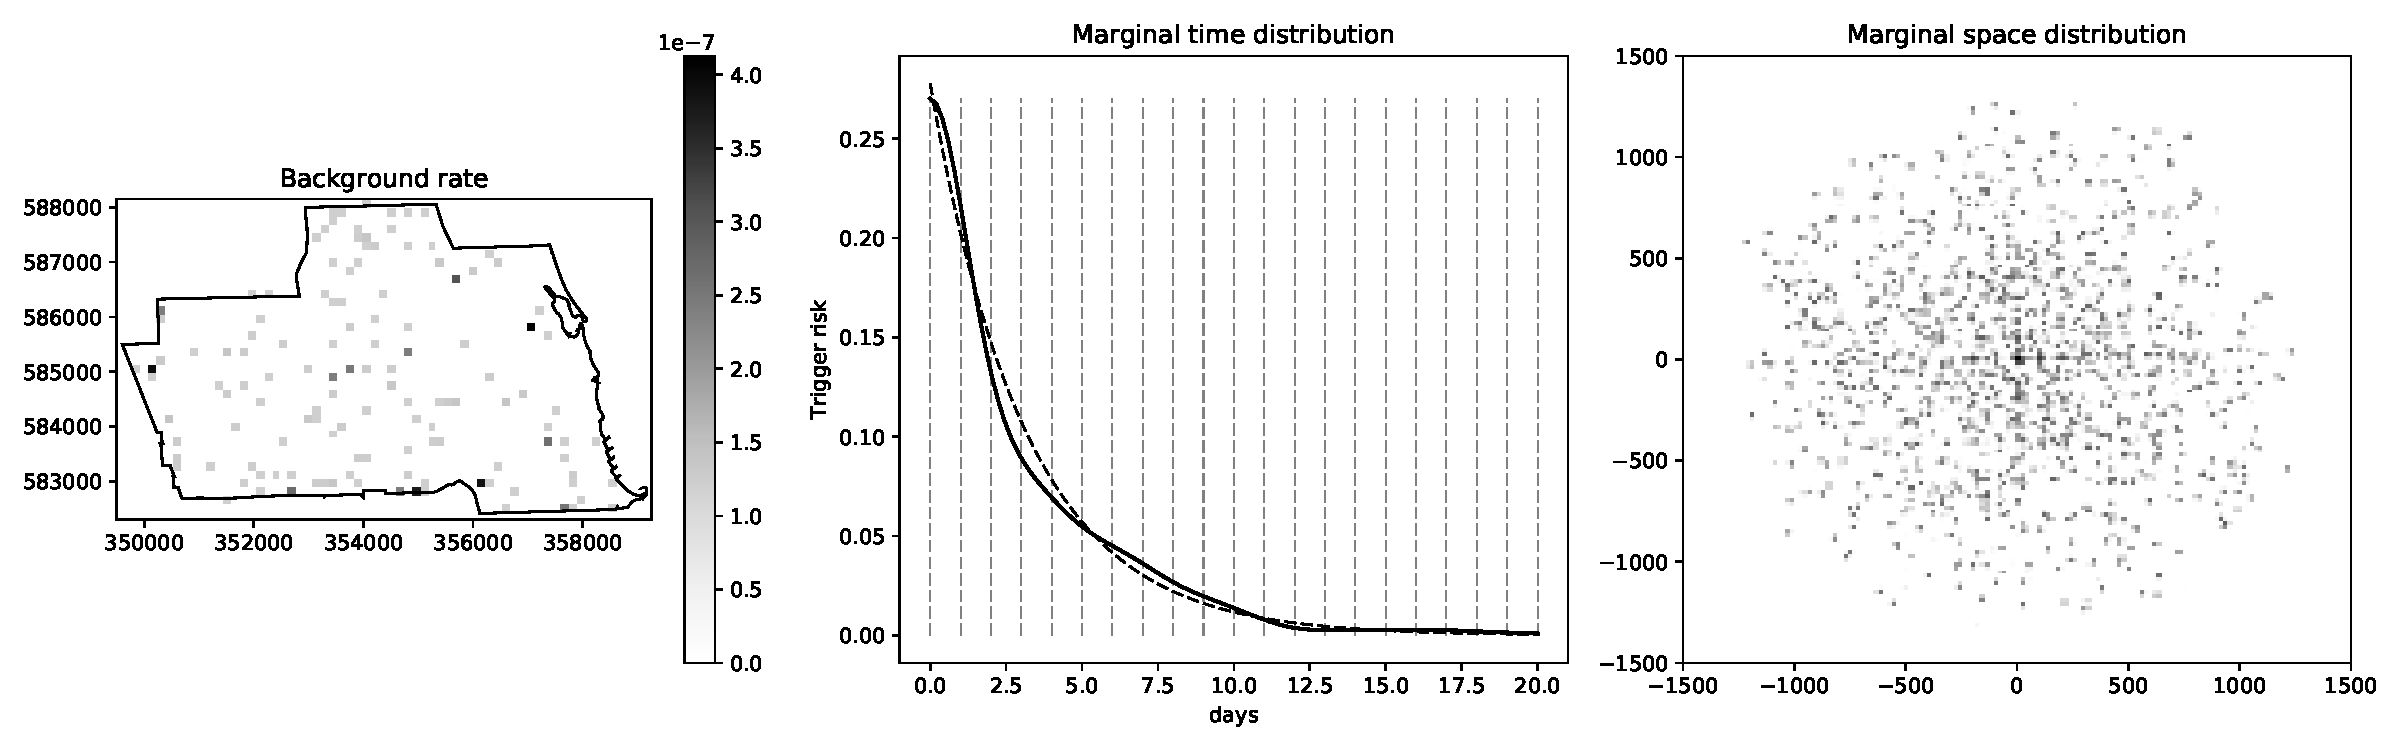
\includegraphics[width=\textwidth]{../notebooks/full_kde_1.pdf}
  \caption{North side of Chicago, for the model described in Section~\ref{sec:joint_grid}.
  We divide the spatial coordinates by 20, and then estimate the combined time/space kernel
  with a bandwidth of 1.}
  \label{fig:full_kde_1}
\end{figure*}

Figure~\ref{fig:full_kde_2} shows slices of the triggering kernel at varying time points,
each normalised by the marginal time kernel at that time.  We see that the space kernel changes
in time, becoming more concentrated as time increases.  This seems counter-intuitive, as we would
expect trigger events to become more dispersed as time went on (to be consistent with the
criminological basis of repeat and near-repeat behaviour).

\begin{figure*}
  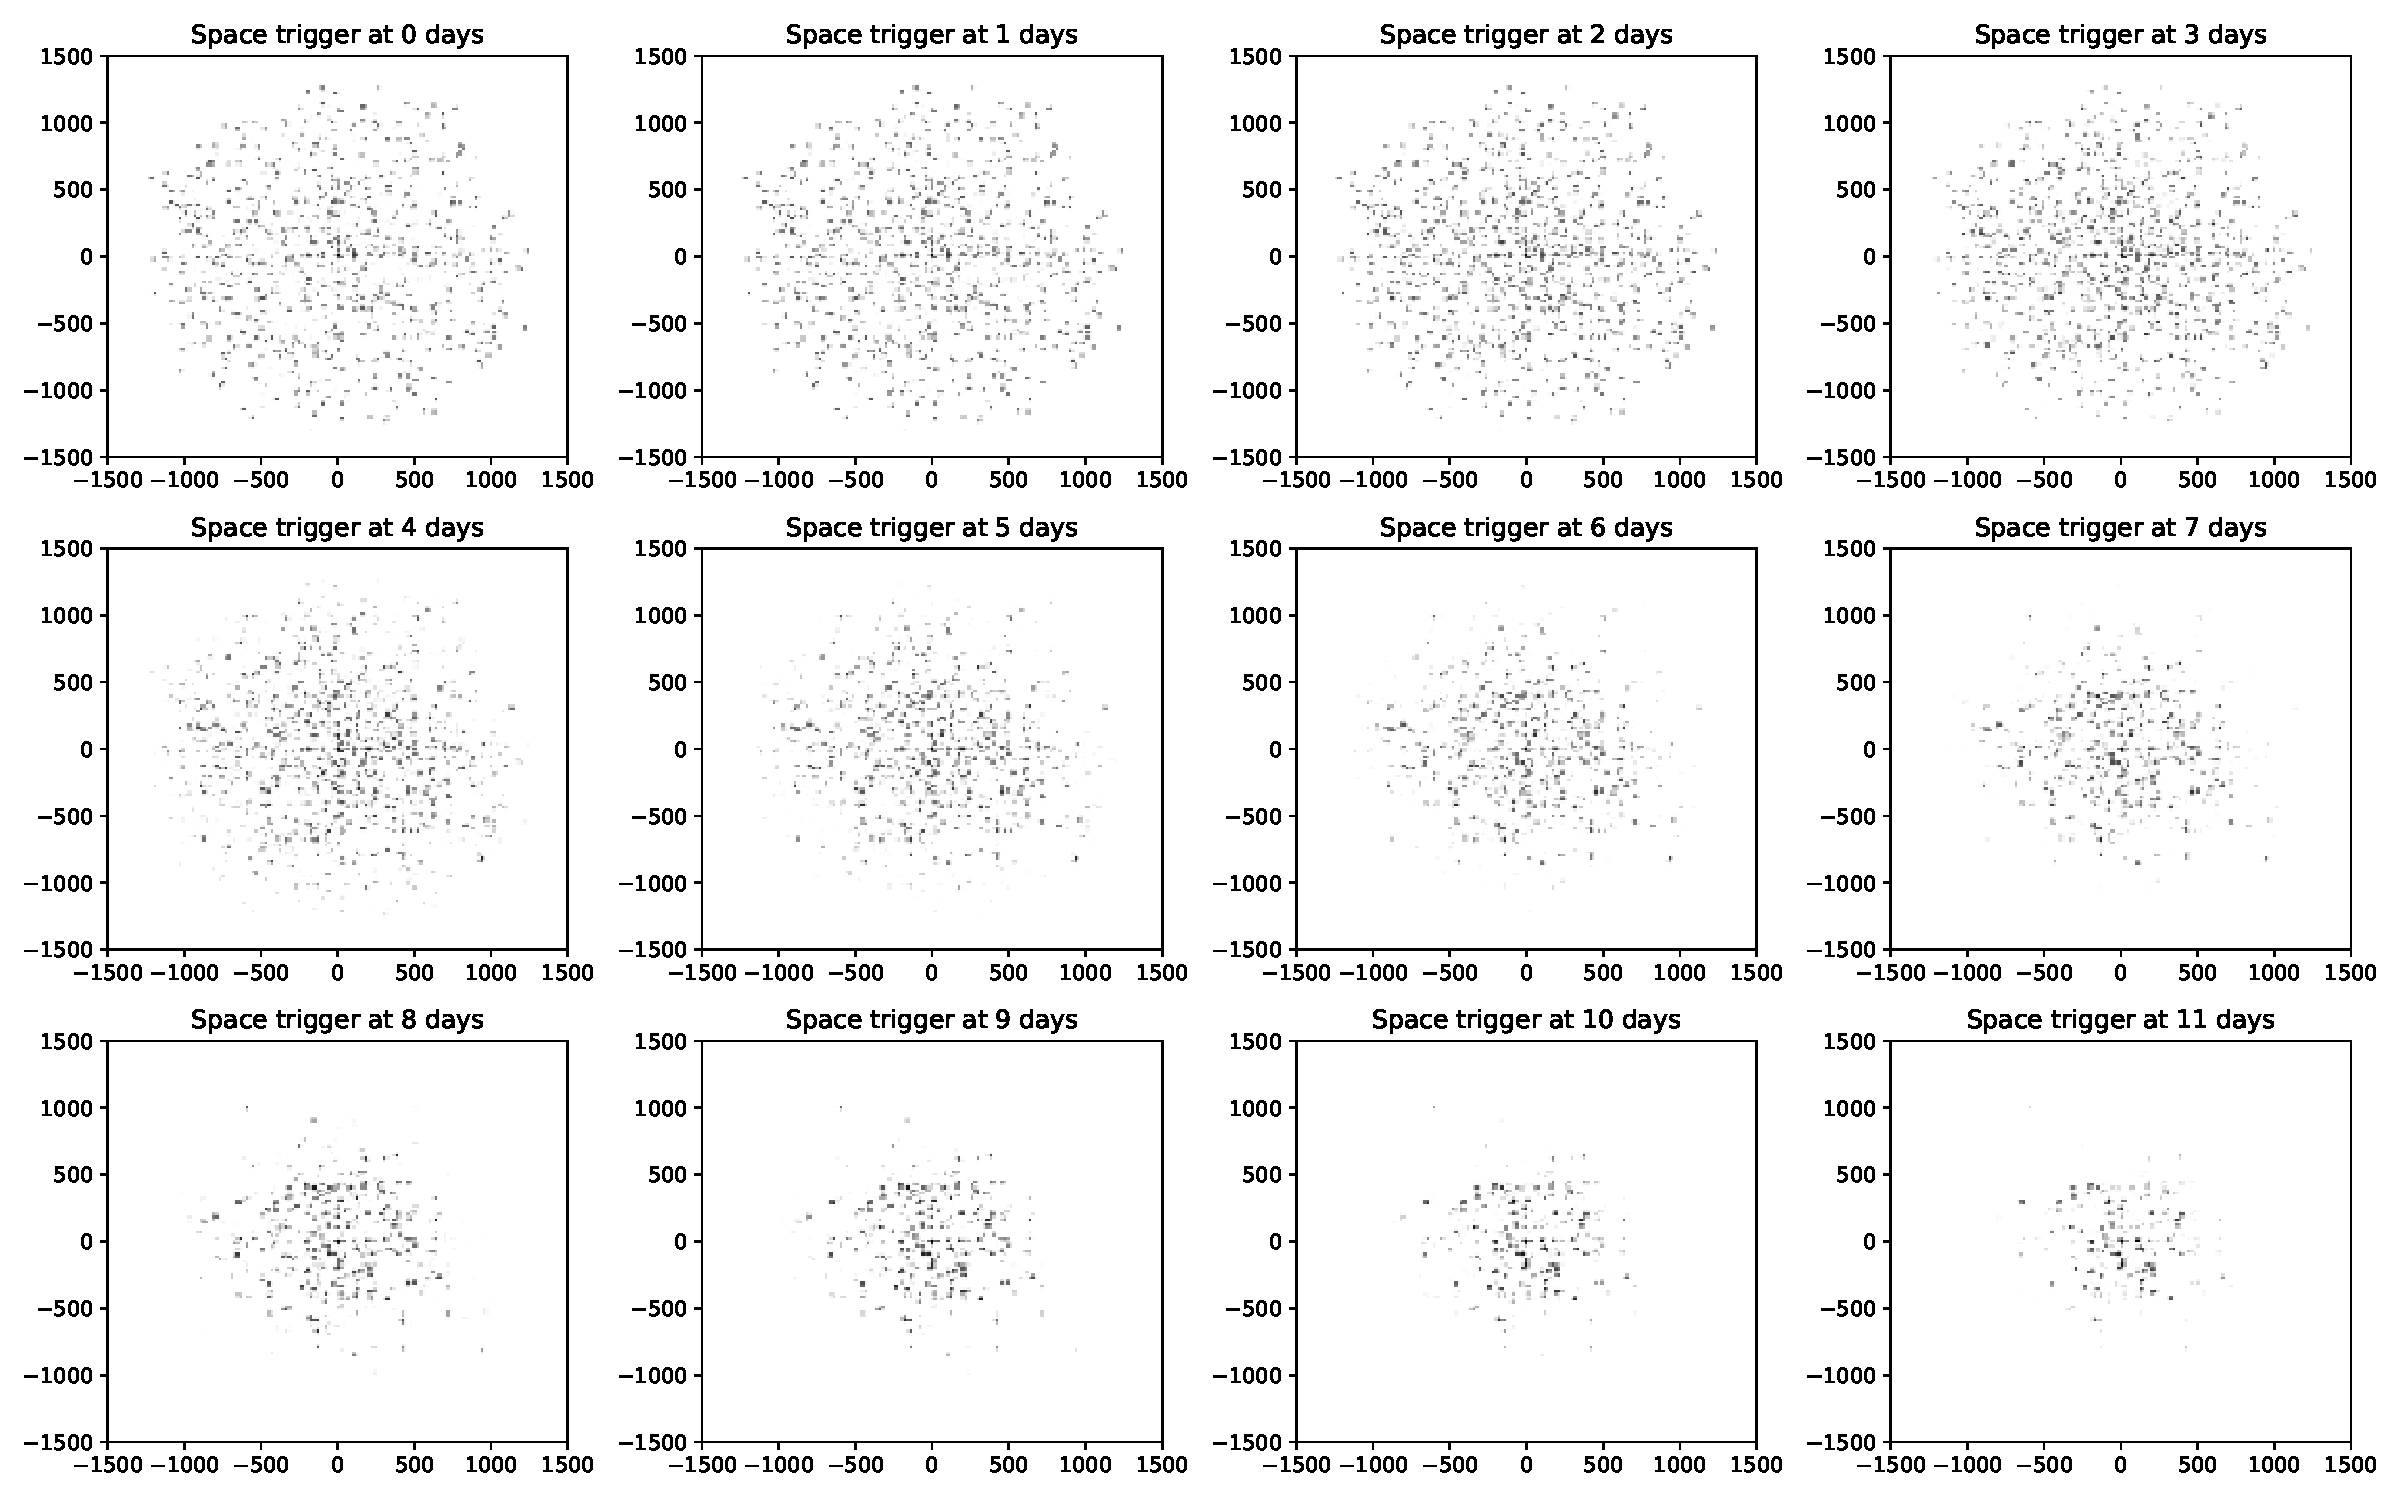
\includegraphics[width=\textwidth]{../notebooks/full_kde_2.pdf}
  \caption{As Figure~\ref{fig:full_kde_1}, showing slices of the triggering kernel at varying time points.}
  \label{fig:full_kde_2}
\end{figure*}

Finally Figure~\ref{fig:full_kde_3} shows the sampled triggered events.  This is similar to
Figure~\ref{fig:grid_kde_1a}, but the space locations are a little more concentrated (within 300m,
instead of 400m) but the grid pattern is a little less evident.  The plots against time show the
increasing spatial concentration with time that we observed before.

\begin{figure*}
  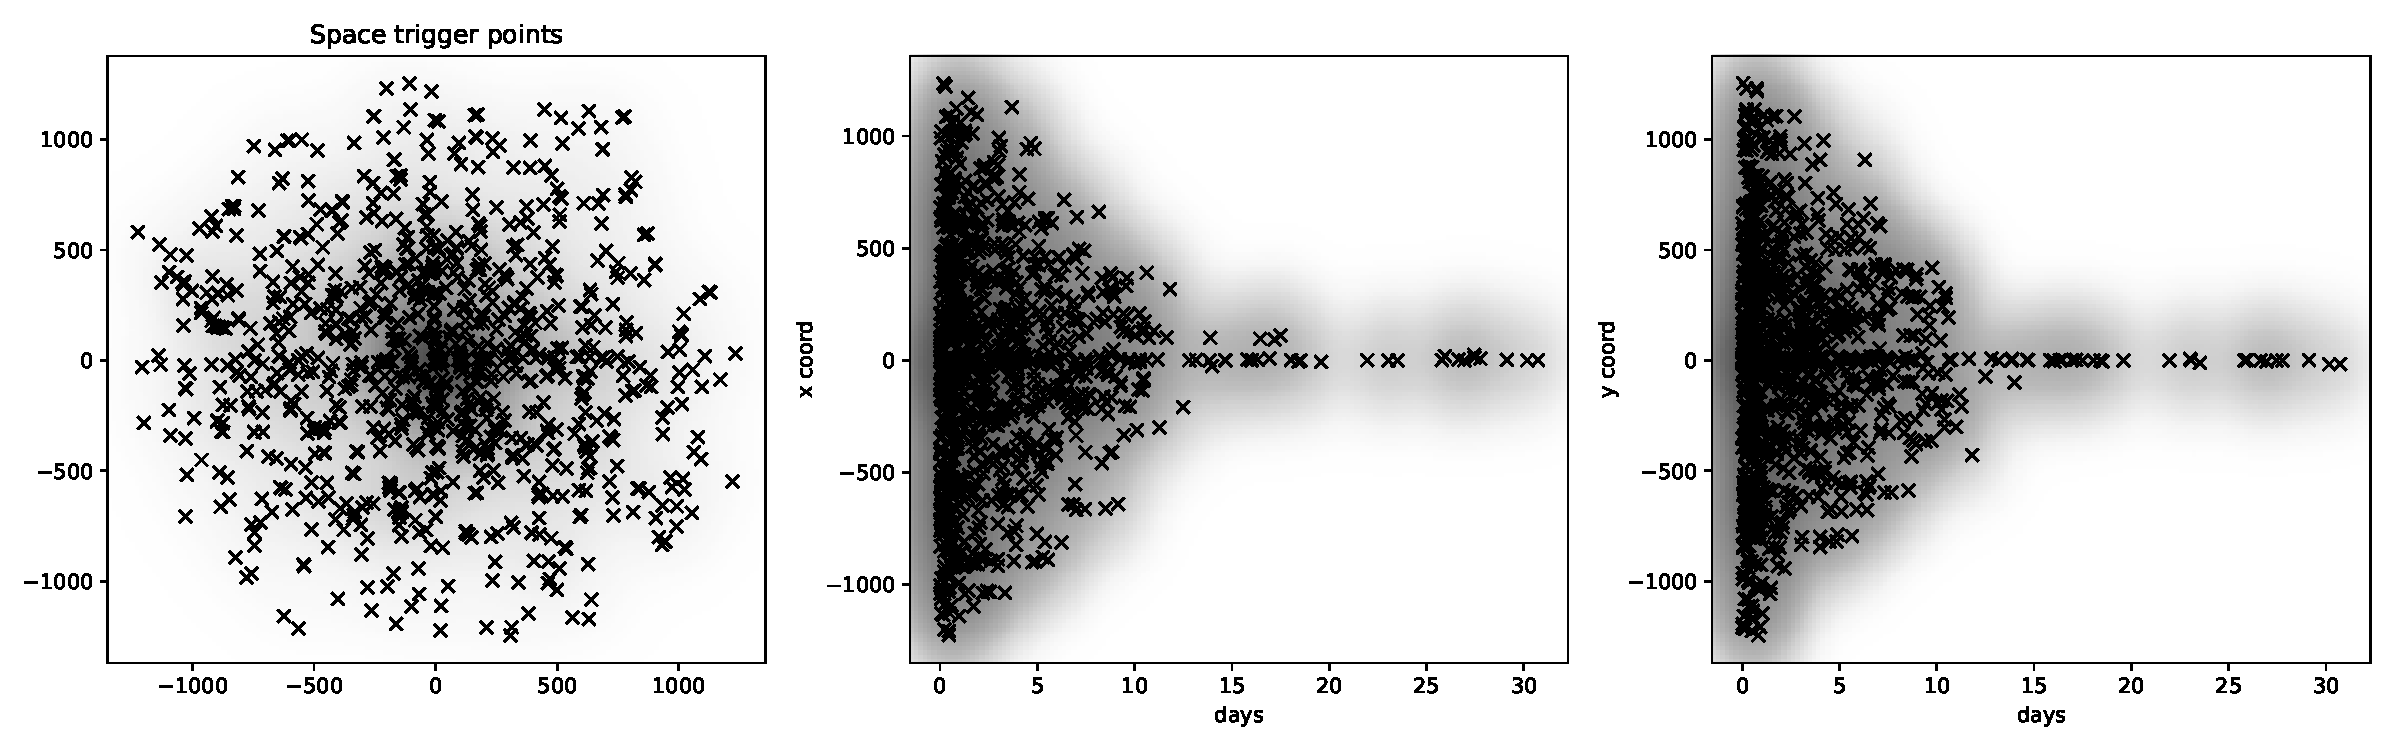
\includegraphics[width=\textwidth]{../notebooks/full_kde_3.pdf}
  \caption{As Figure~\ref{fig:full_kde_1}, showing the sampled trigger events}
  \label{fig:full_kde_3}
\end{figure*}

For the second dataset, the results are rather similar.  The fix of an exponential to the
time kernel is even better, and the marginal space kernel looks very similar, but, again, with
a less pronounced ``grid-like'' pattern.  The version of Figure~\ref{fig:full_kde_2} for the
second dataset is also much the same.  




\subsection{Non-grid based model}\label{sec:no_grid_kde}

The final step towards the model used in \cite{sepp2} is to stop using a grid to estimate
the background rate.  So our general model will be
\[ \lambda^*(t,x,y) = \mu(t,x,y) + \sum_{t_i < t} \mu_1(t-t_i, x-x_i, y-y_i). \]
In \cite{sepp2} $\mu$ is set to to $f(t)g(x,y)$ and $f,g$ are estimated via KDE methods.
A problem here, as explained before, is that KDE methods are suseptible to ``edge-effect'',
which will in particular badly effect $f$ near the start and end of the time period we are
interested in.  As our ultimate aim is prediction, we actually need to project $f$ forwards
(a little) in time.  There are no details in \cite{sepp2} as to how prediction was actually
carried out.  We instead prefer to assume a constant background rate in time.
A more sophisticated analysis, which we do not explore here, would probably use time-series
techniques to identify periodic and overall trend levels in the background rate.

So we work with
\[ \lambda^*(t,x,y) = \mu f(x,y) + \theta \sum_{t_i < t} g(t-t_i, x-x_i, y-y_i), \]
where $\mu$ is the overall background rate, $\theta$ is the triggering rate, and $f,g$
are probability densities.  We will again estimate $f$ and $g$ by KDE methods, and we
reflect $g$ about $0$ in the first variable to take account of time always being positive.

Applied to synthetic data, as in Figure~\ref{fig:sim_grid}, the model fits well, with the
exception that the time trigger is rather underestimated near $0$ (judging from the plots give in
\cite{sepp} and \cite{rc} those authors encountered the same issue).  

We used the same space/time KDE method as in Section~\ref{sec:joint_grid}, and for the background
used a KDE with a fixed bandwidth of 100m.  The result is shown in Figure~\ref{fig:no_grid_kde_1}.

\begin{figure*}
  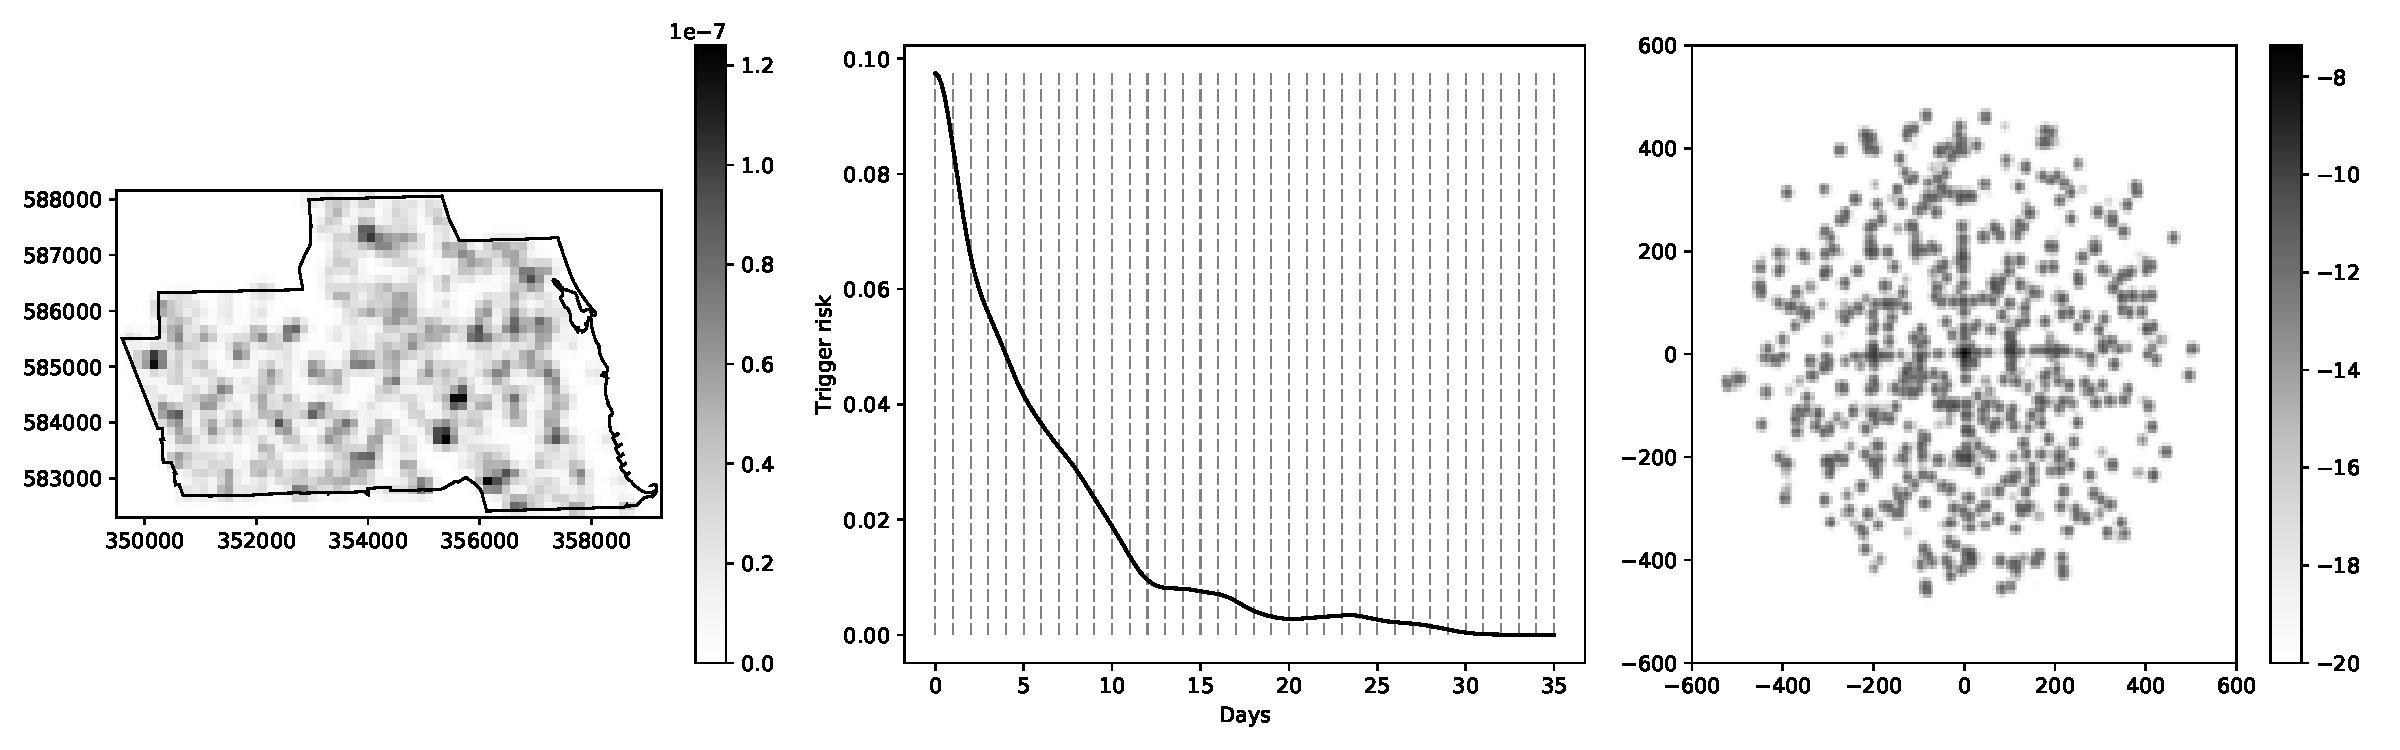
\includegraphics[width=\textwidth]{../notebooks/no_grid_kde_1.pdf}
  \caption{For the model described in Section~\ref{sec:no_grid_kde}, showing the background
rate and the marginal time and space kernels, fitted using the same KDE method as in
Figure~\ref{fig:full_kde_1}, and with a bandwidth of 100m for the background.}
  \label{fig:no_grid_kde_1}
\end{figure*}

[ETC.]


We now also look at
\[ \lambda^*(t,x,y) = \mu f(x,y) + \theta \sum_{t_i < t} g_1(t-t_i) g_2(x-x_i, y-y_i), \]
that is, assume that the trigger factors in space and time.  We have two motivations for this:
speed (as the full three dimensional KDE method is slow to fit, and slow to make predictions
from) and Figure~\ref{fig:full_kde_2} which showed unexpected (and somewhat counter-intuitive)
changes in the space kernel through time.










\section{Making predictions}\label{sec:making_preds}

There is surprisingly little in the crime prediction literature (\cite{sepp, sepp2, rc})
relating to the actual process of translating a model into a prediction.  We have found
the discussion in \cite[Section~1]{vj} to be very helpful in this regard, and we summarise
it now.  We firstly assume that we have a process evolving in time only, with conditional
intensity function $\lambda^*$.  Given data up to a time $T$, we assume we have fitted a
parametric model, or otherwise, and so have knowledge of $\lambda^*(t)$ for $t\leq T$.
We also assume that it makes sense to extrapolate to values $\lambda^*(T+x)$ for $x>0$ small.
To give a concrete example, if we have a Hawkes process with trigger function
$\omega e^{-\omega t}$, compare Appendix~\ref{app:hawkes_em}, then we assume we have settled
on values for $\mu, \theta, \omega$, and so given past events $(t_i)$ we have that
\[ \lambda^*(t) = \mu + \sum_i \theta \omega e^{-\omega (t-t_i)}
\qquad (t>T). \]
The assumption here is that there are no further events in the time interval $[T, T+x)$ which
would add further triggering intensity.

We now use a standard procedure to simulate a point process starting at $T$ with intensity
$\lambda^*(t)$.  In doing this, we must take account of the self-exicited nature of the
process: so each new simulated event will change $\lambda^*$ for times after that event.
However, we do not change the parameters ($\mu, \theta, \omega$ in our example) or non-parametric
functions.  We simulate over the time range we wish to make a prediction for; perhaps the
next day, for example.

We perform such a simulation many times, and, for example, may take an average of the number
of events which occur to get a prediction of the total count of expected events.  Notice
that the self-excited nature of the process means that we cannot simply look at the
value of $\lambda^*(T)$: the history (values of $\lambda^*(T-t)$ for at least small $t>0$)
will be important, as will the triggering process.

We have performed this compute simulation for a number of different parameter combinations.
Figure~\ref{fig:hawkes_sample} shows a window on a simulation with $\mu=2$ and $\omega=1,
\theta=0.5$.

\begin{figure*}
  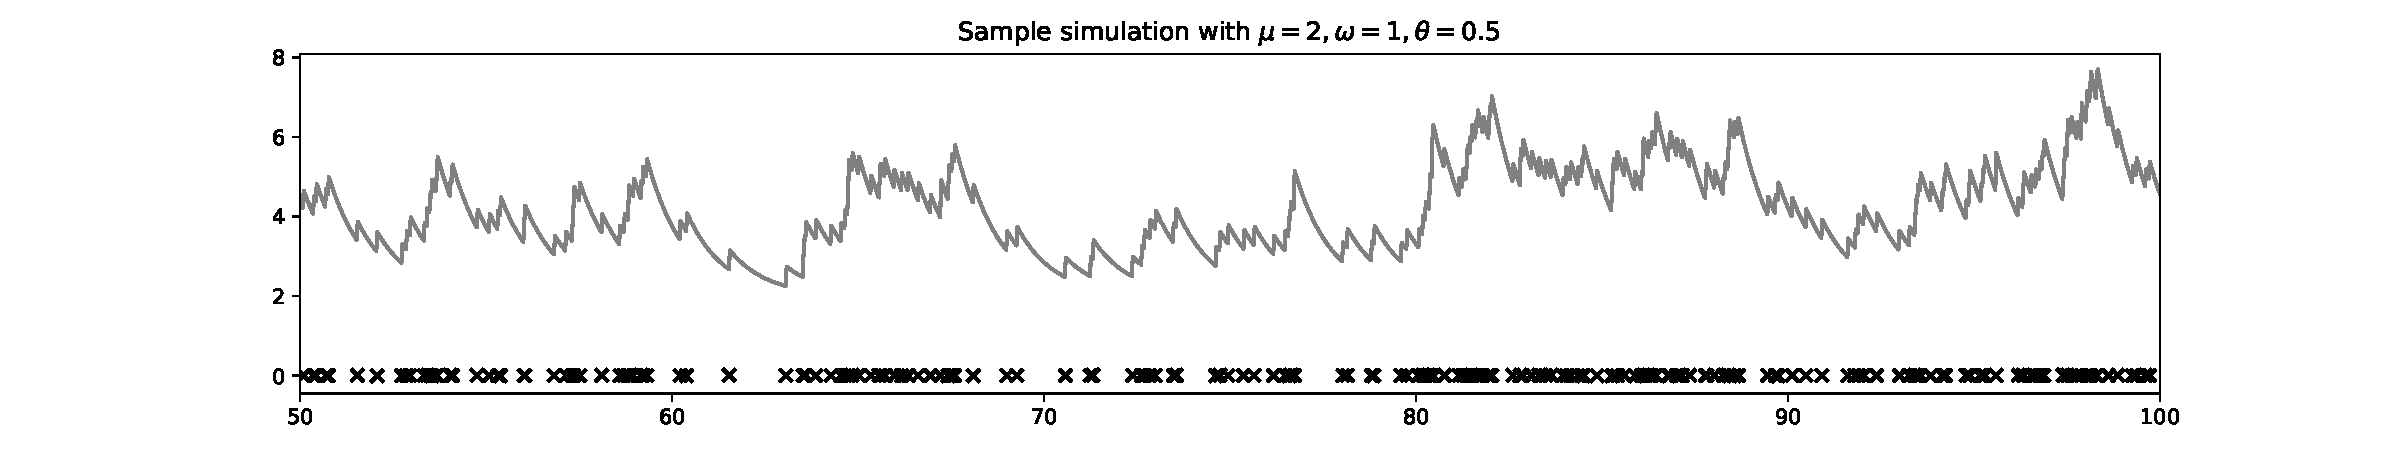
\includegraphics[width=\textwidth]{../notebooks/hawkes_sample.pdf}
  \caption{A simulated Hawkes process, showing the event times and the conditional intensity
function.}
  \label{fig:hawkes_sample}
\end{figure*}

We also performed simulations with $\mu=1,\omega=1,\theta=0.2$ (so less triggering) and
with $\mu=1,\omega=50,\theta=0.5$ (so a rather tighter ``trigger interval'').  In each case
we simulated $1000$ days of events, and then for $T=100$ through $999$ performed our prediction
technique for the next day, the time interval $[T,T+1)$.  We performed 100 such trials for
each day, and take the mean as our prediction.  We also predicted the number of
events simply by integrating the intensity function across this time interval.  For the
parameters we have chosen, we loose very little accuracy by simply evaluating $\lambda^*$ at
$T+1/2$, instead of integrating it between $T$ and $T+1$.
Figure~\ref{fig:hawkes_pred} shows the results of the difference between the predicted
number of events, and the actual number of events.  In all cases, there is a large amount
of error, with a longer tail on the negative side.  This means we often under-estimate, but
more rarely over estimate, which seems intuitively plausible, as it is hard to predict a
large but rare number of triggered events.  The simulation predicion method seems to
perform better, but not by a huge amount, as compared to simply using the mean value
of $\lambda^*$.

\begin{figure*}
  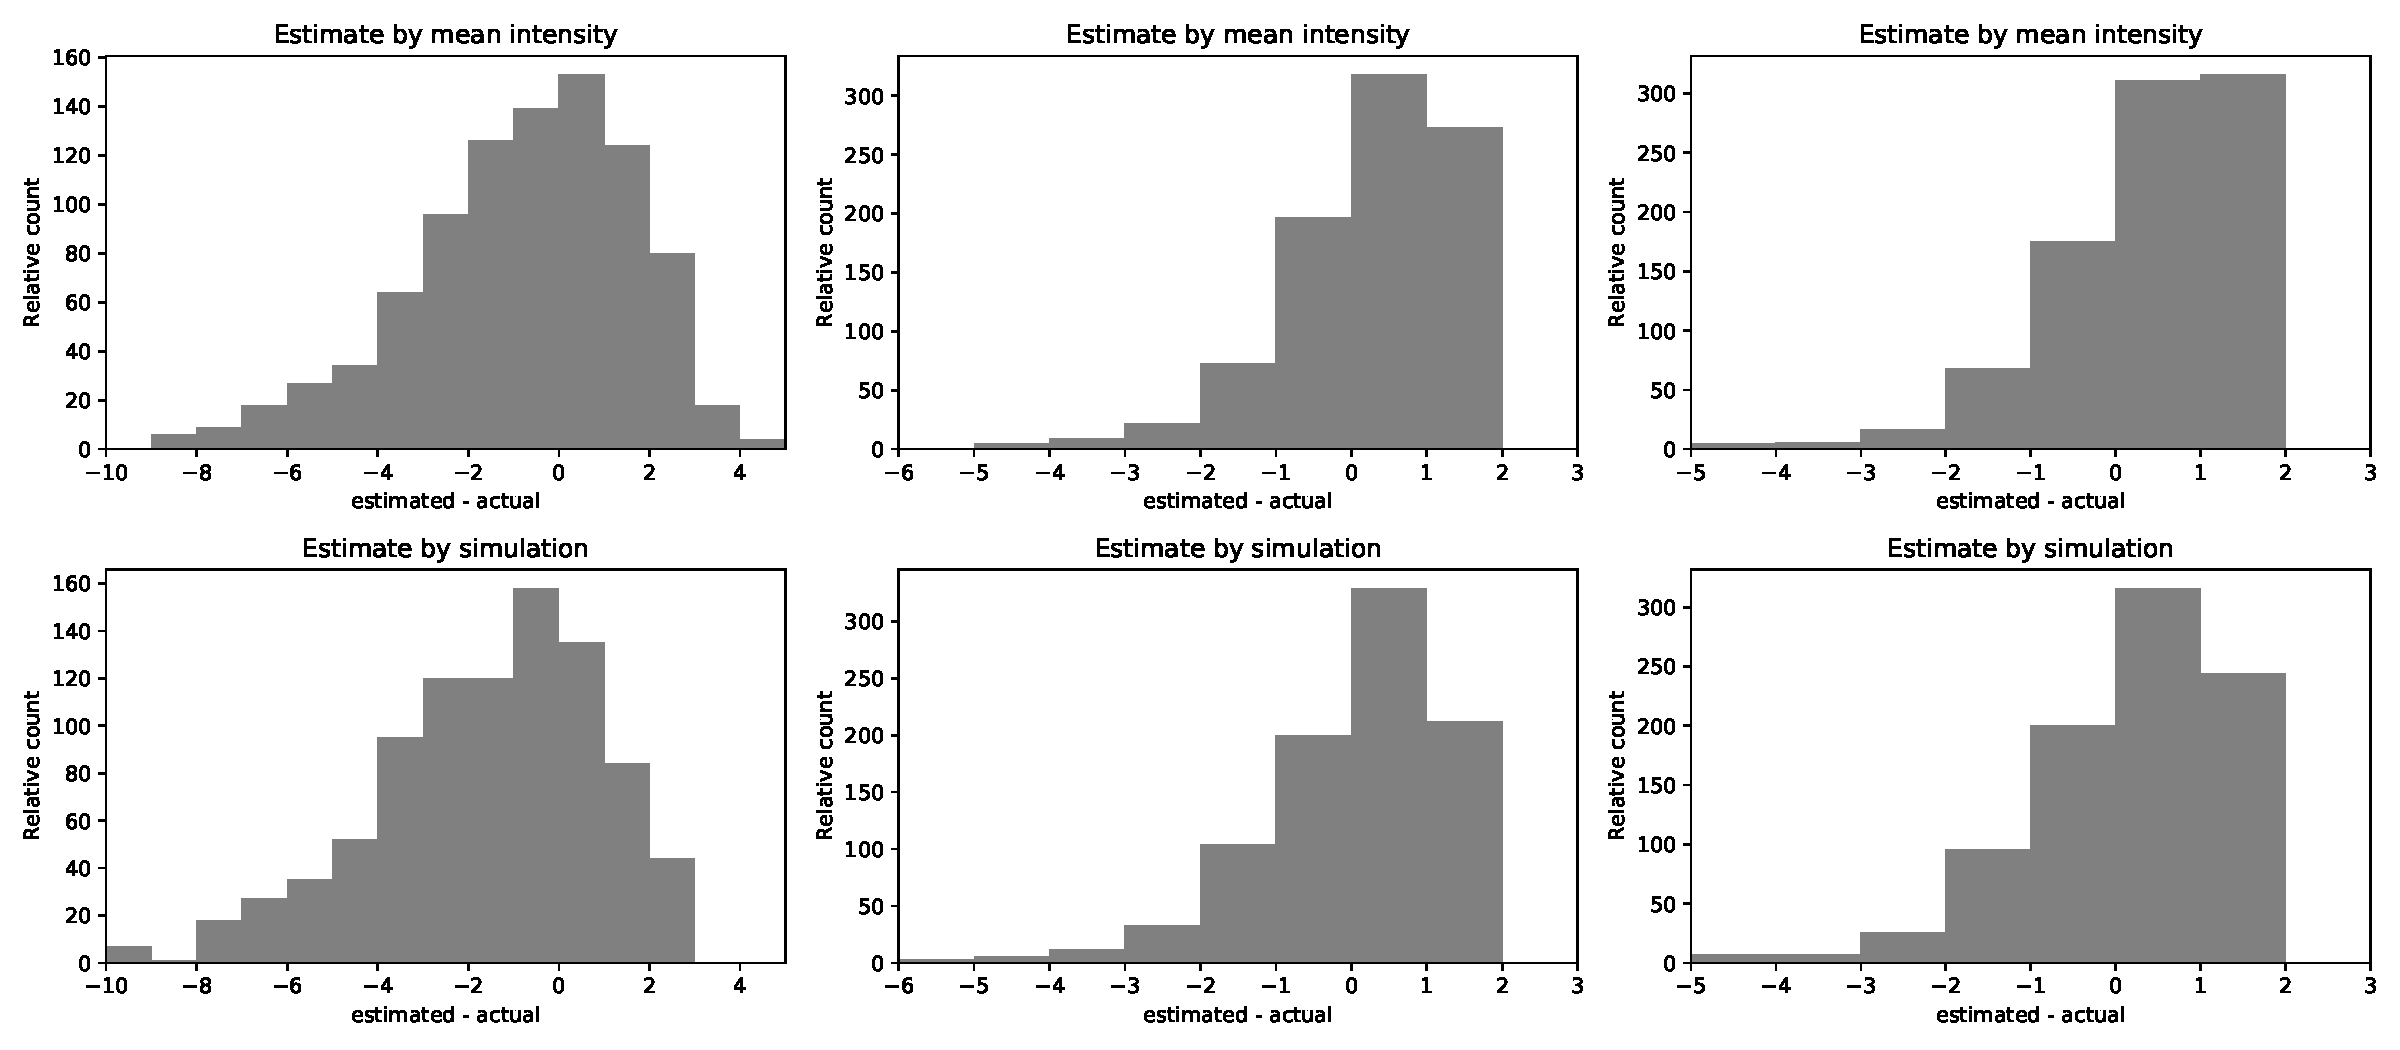
\includegraphics[width=\textwidth]{../notebooks/hawkes_predictions.pdf}
  \caption{Predicting the number of events from a Hawkes process.  Left to right, we have
$\mu=2,\omega=1,\theta=0.5$; $\mu=1,\omega=1,\theta=0.2$; and $\mu=1,\omega=50,\theta=0.5$.}
  \label{fig:hawkes_pred}
\end{figure*}



\subsection{Spatial models}

Extending this to models with a spacial component, there is no difficulty in extending the
simulation.  Suppose we are not interested in the exact occurance times, but rather wish to
obtain a prediction for the likely location of crime events (again, over the next day, for example),
this being the typical output of a crime prediction algorithm.  What our simulation gives us
is many samples of \emph{points}.

We come then to issues discussed in \cite{daws2}.  In this paper, we have been concerned
with specifying probability models and then fitting data to those models.  For a ``prediction''
it is not quite clear what the (implicit) model is.  In \cite{daws2} we decided upon
looking only at grid-based predictions, and essentially a multinomial distribution, with
unknown total intensity.  Thus our study region is divided into $K$ cells, say $(A_k)_{k=1}^K$,
and the ``prediction'' provides a probability $(p_k)$ of crime occurring in cell $A_k$.
We assume that crimes are independent, leading to a multinomial model.  This paper assumes that
crimes are \emph{not} independent, of course, but it is hard to see how to include such
information into a prediction-- it is plainly the case that current prediction methods make
no attempt to model this.

From each simulation $i$, we can calculate the number of events which occurred in cell $k$, say
$n_k^{(i)}$.  Notice that the simulation also tells us the total event count, $n_i=\sum_k n^{(i)}_k$,
but current prediction systems do not concern themselves with trying to predict the total
event count.  If we make the simplifying assumption that each sample is from a multinomial, then the
maximum likelihood estimation of $p_k$ is simply
\[ \hat p_k = \sum_i n_k^{(i)} / \sum_i n_i. \]
If we instead use $\lambda^*$ directly, for example integrating it over both the time interval and
each grid cell, then we obtain expected counts $(n_k)$ say, and the maximum likelihood estimation
is now $\hat p_k = n_k / \sum_k n_k$.

\section{Prediction results}

TODO: I guess compare lots of model, via Hit rate maybe, and see if there is much difference?

Would also be interesting to fix the trigger kernel (e.g. using Prohotspot etc.) and use
the EM algorithm to predict the background, and then make predictions.

TODO: Making a prediction from a KDE method is very slow. (Very slow!)  Can we discretise the trigger kernel, and use that instead to make the prediction?  Is that faster?  Is it as good?



\appendix
\section{Appendix}

In the appendix, we give a brief, but relatively self-contained, guide to the probability
theory behind the point process models we consider, and outline the Expectation
Maximisation (EM) algorithm we apply to fit models.


\subsection{Point processes}\label{app:pp}

We shall treat point processes via their \emph{conditional intensity functions}.
Let us first consider a point process evolving only in time, where events occur at times
$0 < t_1 < t_2 < \cdots $ and carry no further information.  In probability theory, a point
process is a ``random'' collection of times, satisfying certain mild conditions.  Let $N(t)$
be the \emph{counting process} of the point process, that is, $N(t)$ is the random variable
giving the number of events which have occurred before time $t$.  The conditional intensity 
function (or sometimes, \emph{hazard function}) is, intuitively speaking,
\[ \lambda^*(t) = \lim_{h\rightarrow 0} \frac{\mathbb E[ N(t+h) - N(t) | \mc H_t ]}{h}. \]
Here $(\mc H_t)_{t\geq 0}$ is the filtration forming the history of the process; we write 
$\lambda^*$ and not $\lambda$ to stress this dependence on the past.
That is, conditional on what has occurred before time $t$, we think of
$\lambda^*(t) \ \rd t$ as being the expected number of events which will occur near time
$t$ times an infinitesimal length of time.  Under reasonable conditions, the conditional 
intensity function exists, and when it exists, it uniquely characterises the point process.

For example, if $\lambda^*(t) = \mu$ independent of time, we have a homogeneous Poisson
process when intensity $\mu$ (the expected number of events in any unit interval of time is
$\mu$).  If $\lambda^*(t) = \mu(t)$ is a function of time, but independent of the past, 
then we have an inhomogeneous Poisson process.  A more interesting example is the \emph{Hawkes}
process where
\[ \lambda^*(t) = \mu + \alpha \sum_{t_i < t} e^{-\beta(t-t_i)}. \]
We think of this as a combination of a fixed ``background'' rate $\mu$ and then a 
``self-exciting'' component, one for each past event, of the form $\alpha e^{-\beta(t-t_i)}$.
Thus, immediately after an event occurs, the intensity increases (which makes it more likely
that further events will occur) but this decays exponentially in time (meaning that, almost
surely, the self-exciting ``cascade'' will end and we will not have an infinite number of
events occurring in finite time, so long as $\alpha < \beta$).

For treating point processes in many dimensions, we find it useful to work with ``marked
processes'' which we think of as a point process evolving in time, where each event carries
extra information: the ``mark'' (here almost exclusively 2D coordinates $(x,y)$).  
We shall only consider models with conditional intensity functions of the form
\begin{equation}
\lambda^*(t,x,y) = \mu(t,x,y) + \sum_{t_j<t} \mu_1(t_j,x_j,y_j;t-t_j,x-x_j,y-y_j).
\label{eq:main}
\end{equation}
Here we have an inhomogeneous background process, and each event in the past adds,
independently and linearly, to the total with a function $\mu_1$ which depends on the
location of the historical event, and the vector from the event to the location of interest.
As we discussed in the introduction, in this paper, we shall actually only consider
the case when $\mu_1$ only depends on $(t-t_i,x-x_i,y-y_i)$ and not the absolute location.

Suppose $(t_i,x_i,y_i)_{i=1}^n$ is a realisation of a point process in the time interval
$[0,T]$.  The likelihood $L$ is
\[ L = \Big( \prod_{i=1}^n \lambda^*(t_i,x_i,y_i)\Big)
\exp\Big(-\int_0^T \int_{\mathbb R^2} \lambda^*(t,x,y) \ \rd x \rd y \ \rd t\Big). \]
With $\lambda^*$ of the above form, each term in the product is the sum of a $\mu$
term and $i-1$ terms involving $\mu_1$.  Let $Z$ be the collection of all choices of
integers $(z_i)_{i=1}^n$ with $1 \leq z_i \leq i$ for each $i$.  If we fully multiply out
the product, then we end with summands indexed by $Z$, where the choice $z_i=i$ corresponds
to choosing the $\mu$ term for index $i$, and the choice $j=z_i<i$ corresponds to choosing
the term $\mu_1(t_j,x_j,y_j,t_i-t_j,x_i-x_j,y_i-y_j)$.  For example, with $n=2$, and dropping
the $x$ and $y$ parts for clarity, we find
\[ \lambda^*(t_1)\lambda^*(t_2) = \mu(t_1)\mu(t_2) + \mu(t_1)\mu_1(t_1, t_2-t_1) \]
where the summands correspond to the choices $z_1=1,z_2=1$ and $z_1=1,z_2=2$.

The integral in the exponential term may be computed in an iterative way.  Again for
clarify we shall ignore the $x$ and $y$ parts for the moment, to find that
\[ \int_0^T \lambda^*(t) \ \rd t 
= \int_0^{t_1} \mu(t)  \ \rd t 
+ \int_{t_1}^{t_2} \mu(t) + \mu_1(t_1, t-t_1) \ \rd t
+ \cdots + \int_{t_n}^T \mu(t) + \sum_{j=1}^n \mu_1(t_j, t-t_j) \ \rd t. \]
This may be re-written as 
\[ \int_0^T \mu(t) \ \rd t + \sum_{j=1}^n \int_{t_j}^T \mu_1(t_j, t-t_j) \ \rd t
= \int_0^T \mu(t) \ \rd t + \sum_{j=1}^n \int_{0}^{T-t_j} \mu_1(t_j, t) \ \rd t. \]

Thus the likelihood is equal to
\begin{align}
\sum_{z\in Z} \prod_{j=1}^n \big( \mu(t_j)[z_j=j] &+ \mu_1(t_{z_j},t_j - t_{z_j}) [z_j<j] \big)
\notag \\ &
\exp\Big(-\int_0^T \mu(t) \ \rd t\Big) \prod_{j=1}^n\exp\Big(-\int_{0}^{T-t_j} \mu_1(t_j, t) \ \rd t\Big), \label{eq:one}
\end{align}
where $[z_j=j]$ is the random variable (the Iverson bracket) taking the value $1$ when
$z_j=j$ and $0$ otherwise, and similarly for $[z_j<j]$.

This form of the likelihood has an interesting interpretation, which has obvious links with how
to \emph{simulate} such a point process, see the discussion in \cite{mr, mr1}.
Given $z$ let $Z_0 = \{ j : z_j=j \}$ so we have the term
\[ \prod_{j\in Z_0} \mu(t_j) \exp\Big(-\int_0^T \mu(t) \ \rd t\Big). \]
This is nothing but the likelihood of an inhomogeneous Poisson process-- these are the
``background'' events.  For $i$ set $Z_i = \{ j > i : z_j=i \}$ so we have the term
\[ \prod_{j\in Z_i} \mu_1(t_i,t_j - t_i)\exp\Big(-\int_{0}^{T-t_i} \mu_1(t_i, t) \ \rd t\Big). \]
This is the likelihood of an inhomogeneous Poisson process with intensity $\mu_1(t_i,\cdot)$
starting at time $t_i$.  These are the events ``triggered'' by event $t_i$.

We have hence simplified the form of the likelihood, given the ``branching structure'' of
the process, encoded in the random variable $z$.  We cannot observe $z$ directly, but this form
allows us to apply the \emph{Expectation Maximisation} algorithm, \cite{mk}.


\subsection{The Expectation Maximisation algorithm}\label{app:em}

The Expectation Maximisation algorithm is a general technique giving iterative algorithms
for parameter estimation for problems which have ``unobserved data''.  Each iterative step
has two stages:
\begin{itemize}
\item The \emph{expectation} (or ``E'') step.  Given the observed data, we compute the
conditional expectation of the log likelihood over the hidden data $z$.  When computing the
conditional expectation, we use the \emph{current} estimate of the parameters.
\item The \emph{maximisation} (or ``M'') step.  We now maximise the resulting function
in the parameters, giving new estimates for the parameters.
\end{itemize}
Under mild conditions, each step is guaranteed to increase the likelihood, but convergence
can be slow, and it is possible to converge only to a local maximum.

In our case, given the above remarks, we find that
\[ \mathbb P((z_i) | (t_i),(x_i),(y_i)) = \prod_{i=1}^n p_{j,i} \]
where
\[ p_{j,i} = \mathbb P(z_i=j\leq i) = \begin{cases} \mu(t_i,x_i,y_i) / \lambda^*(t_i,x_i,y_i) &: j=i, \\
\mu_1(t_j,x_j,y_j; t_i-t_j,x_i-x_j,y_i-y_j) / \lambda^*(t_i,x_i,y_i) &: j<i \end{cases} \]
Here $\lambda^*(t_i,x_i,y_i)$ is the normalisation factor ensuring that $\sum_{i=1}^n p_{i,j} = 1$ for
each $j$.  The (general) E step is hence to compute
\begin{equation}
\Psi = \mathbb E_z(\log L) = 
\sum_z \log L((t_i),(x_i),(y_i),(z_i))  \prod_i p_{z_i,i},
\label{eq:factors}
\end{equation}
and then the M step is to optimise $\Psi$.  Here $\mu$ and $\mu_1$ will depend on parameters
which will be fixed for the purposes of computing the terms $p_{j,i}$, but will be
variable when maximising $\Psi$.

It will be convenient to factor $\mu$ and $\mu_1$ as
\[ \mu(t,x,y) = \mu(t) f(x,y|t), \quad \mu_1(t,x,y;t',x',y')
= \mu_1(t,x,y;t') g(x',y';t,x,y,t') \]
where $\mu(t) = \int_{\mathbb R^2} \mu(t,x,y) \ \rd x \rd y$ and $f(x,y|t) = \mu(t,x,y) / \mu(t)$ for
$\mu(t)>0$; and similarly for $\mu_1$ and $g$.  Notice that then $f$ and $g$ are
\emph{probability} densities.  

From (\ref{eq:one}) above (with dependence on $x,y$ now included) we see that
\begin{align*} \Psi &= \mathbb E_z\Big(
\sum_{j=1}^n \log \big( \mu(t_j)f(x_j,y_j|t_j)[z_j=j]
	\\ &\qquad\qquad + \mu_1(t_{z_j},x_{z_j},y_{z_j};t_j - t_{z_j})
	g(x_j - x_{z_j},y_j - y_{z_j}; t_{z_j},x_{z_j},y_{z_j},t_j - t_{z_j}) [z_j<j] \big)
\\ &\qquad\qquad\qquad
-\int_0^T \mu(t) \ \rd t - \sum_{j=1}^n\int_{0}^{T-t_j} \mu_1(t_j, t) \ \rd t
\Big).
\end{align*}
Using linearity of the expectation, this is equal to
\begin{align}
\Psi=&\sum_{j=1}^n p_{j,j} \log \big( \mu(t_j)f(x_j,y_j|t_j)\big)
    - \int_0^T \mu(t) \ \rd t \notag\\
+ &\sum_{j=1}^n \sum_{i<j} p_{i,j}
	\log\big(\mu_1(t_i,x_i,y_i;t_j - t_i)
	g(x_j - x_i,y_j - y_i; t_i,x_i,y_i,t_j - t_i) \big)
\notag\\ & \qquad\qquad
- \sum_{j=1}^n\int_{0}^{T-t_j} \mu_1(t_j, t) \ \rd t. \label{eq:two}
\end{align}
As we shall see shortly in examples, in practice, this form allows us to optimise
the parameters for, say, $\mu$, without needing to consider $f,\mu_1$ or $g$.

To our knowledge, \cite{vs} was the first article to explore the EM algorithm in
the setting of self-excited point processes.  Unfortunately, \cite{vs} uses different
notation to later works, and treats only the ``ETAS'' model.  We prefer to present
a rather general construction which can be specialsed to many models.


\subsection{Allowing exact repeats, in time}\label{app:exact_repeats_in_time}

Looking again at equation (\ref{eq:main}) defining our model, we sum over only those
events $t_j<t$.  We can consequently make sense, at least in a formal way, of
realisations $(t_i)$ where merely $t_1 \leq t_2 \leq \cdots \leq t_n$.  In the EM
algorithm, this corresponds to summing over not just $i<j$ but also $t_i < t_j$.
Equivalently, we may set $p_{i,j}=0$ for $i<j$ when $t_i = t_j$.


\subsection{Expected number of triggered events}\ref{app:gen_func}

Let $\theta = \int \mu_1$ be the total intensity of the trigger.  The expected number of
events that the trigger kernel will give rise to is thus $\theta$.
Let $Z_0=1$ be the an event, which triggers $Z_1 \geq 0$ further events.  Each of
these events triggers further events, independently, say giving a total of $Z_2\geq 0$
further events, and so forth.  We thus have a \emph{branching process}, \cite[Section~5.4]{gs},
and so by using generating functions, we can prove that $\mathbb E(Z_n) = \mu^n$, and hence
that the expected total number of triggered events is $\mu + \mu^2 + \mu^3 + \cdots
= \mu(1-\mu)^{-1}$ as claimed in the main text.



\subsection{Fully parametric example}\label{app:hawkes_em}

This example is the model used in \cite[Section~2]{lm}.
We shall again ignore spatial components.
Here we set $\mu$ to be a constant, and let the triggering kernel have the form
\[ \mu_1(t_i; t - t_i) = \theta \omega e^{-\omega(t-t_i)}, \]
where $\theta, \omega$ are parameters (along with $\mu$) to be estimated.
We find that
\begin{align*} \Psi &= \sum_{j=1}^n p_{j,j} \log\mu - \int_0^T \mu \ dt
+ \sum_{i<j} p_{i,j} \big( \log\theta + \log\omega - \omega(t_j-t_i) \big)
- \sum_{j=1}^n \int_0^{T-t_j} \theta \omega e^{-\omega t} \ dt \\
&= \sum_{j=1}^n p_{j,j} \log\mu - \mu T
+ \sum_{i<j} p_{i,j} \big( \log\theta + \log\omega - \omega(t_j-t_i) \big)
- \theta \sum_{j=1}^n \big(1 - e^{-\omega (T-t_j)}\big).
\end{align*}
Maximising in $\mu$ gives $\mu = \frac{1}{T} \sum_j p_{j,j}$, and similarly we find
\[ \theta = \frac{\sum_{i<j} p_{i,j}}{\sum_j 1 - e^{-w(T-t_j)}}, \qquad
\omega = \frac{\sum_{i<j} p_{i,j}}{\sum_{i<j} p_{i,j} (t_j-t_i) + \theta\sum_j (T-t_j)e^{-\omega(T-t_j)}}. \]
In the expression for $\theta$ we use the \emph{previous} estimate for $\omega$, and similarly
for $\omega$.

It is often assumed that $e^{-w(T-t_j)}$ is small for all $j$, giving the simplifications
\[ \theta = \frac{\sum_{i<j} p_{i,j}}{n}, \qquad
\omega = \frac{\sum_{i<j} p_{i,j}}{\sum_{i<j} p_{i,j} (t_j-t_i)}. \]



\subsection{With a spatial component}\label{app:grid_model_em}

Following \cite[Section~2.2]{sepp2} we now introduce a spatial component.
We assume that events occur in regions $k=1,\cdots,K$, where region $k$ has background rate
$\mu_k$, but that all regions share the same ``triggering parameters'' $\theta$ and $\omega$.
We assume that events in region $k$ only trigger future events in the same region.
Let the events $(t_i, x_i, y_i)$ be such that $(x_i,y_i)$ occurs in region $k(i)$.  Thus
\[ \lambda^*(t_i,x_i,y_i) = \mu_{k(i)} + \sum_{j<i, k(j)=k(i)} \theta \omega e^{-\omega(t_i-t_j)}. \]
We can similarly compute the integral
\begin{align*}
\int_0^T \int_{\mathbb R^2} \lambda^*(t,x,y) \ \rd x \rd y \ \rd t
&= \int_0^T \sum_{k=1}^K \int_{\text{region }k} \Big( \mu_k + \sum_{t_i < t, k(i)=k}
   \theta \omega e^{-\omega(t-t_i)} \ \rd t \Big) \\
&= \sum_{k=1}^K A_k \Big( T\mu_k + \int_0^T \sum_{t_i < t, k(i)=k}
   \theta \omega e^{-\omega(t-t_i)} \ \rd t \Big)
\end{align*}
where region $k$ has area $A_k$.  Let us group the data by region, say
region $k$ have events which occur at times $(t^{(k)}_i)_{i=1}^{n(k)}$.  Then the
above integral becomes
\begin{align*} \sum_{k=1}^K TA_k\mu_k &+ \sum_{k=1}^K A_k \sum_{i=1}^{n(k)}
\int_0^{T-t^{(k)}_i} \theta\omega e^{-\omega t} \ dt \\
&= \sum_{k=1}^K TA_k\mu_k + \sum_{k=1}^K \theta A_k \sum_{i=1}^{n(k)}
\big( 1 - e^{-\omega (T-t^{(k)}_i)} \big).
\end{align*}

From (\ref{eq:two}), we find that
\begin{align*} \Psi &=
\sum_{k=1}^K \log(\mu_k) \sum_{j=1}^{n(k)} p^{(k)}_{j,j} - \sum_{k=1}^K TA_k\mu_k\\
&+ \sum_{k=1}^K \sum_{1\leq i<j\leq n(k)} p^{(k)}_{i,j} \log\big( \theta\omega
  e^{-\omega(t^{(k)}_j - t^{(k)}_i)} \big) - \sum_{k=1}^K \theta A_k \sum_{i=1}^{n(k)}
\big( 1 - e^{-\omega (T-t^{(k)}_i)} \big)
\end{align*}
Here
\[ p^{(k)}_{j,j} = \mu_k / \lambda^*_k(t^{(k)}_j), \quad
p^{(k)}_{i,j} = \theta\omega e^{-\omega(t^{(k)}_j - t^{(k)}_i)} / \lambda^*_k(t^{(k)}_j)
\]
where $\lambda^*_k(t) = \mu_k + \sum_{t^{(k)}_i<t} \theta\omega e^{-\omega(t-t^{(k)}_i)}$.

Maximising in $\mu_k$ and $\theta$ gives
\[ \mu_k = \frac{1}{T A_k} \sum_{j=1}^{n(k)} p^{(k)}_{j,j},
\qquad
\theta = \frac{\sum_k \sum_{i<j} p^{(k)}_{i,j}}{\sum_k A_k \sum_i (1-e^{-\omega(T-t^{(k)}_i)})},
\]
and maximising in $\omega$ gives
\[ \omega = \frac{\sum_k \sum_{i<j} p^{(k)}_{i,j}}{
\sum_k \sum_{i<j} p^{(k)}_{i,j} (t^{(k)}_j - t^{(k)}_i)
+ \sum_k \theta A_k \sum_i (T-t^{(k)}_i) e^{-\omega(T-t^{(k)}_i)}
}. \]

If we assume $A_k=A$ for all $k$, then we can absorb the $A$ constant into each $\mu_k$
and $\theta$, and assume that $A=1$.  If we further assume that $e^{-\omega(T-t^{(k)}_i)}=0$
for each $k,i$ then we obtain
\[ \mu_k = \frac{1}{T} \sum_{j=1}^{n(k)} p^{(k)}_{j,j},
\quad
\theta = \frac{\sum_k \sum_{i<j} p^{(k)}_{i,j}}{n},
\quad
\omega = \frac{\sum_k \sum_{i<j} p^{(k)}_{i,j}}{
\sum_k \sum_{i<j} p^{(k)}_{i,j} (t^{(k)}_j - t^{(k)}_i)}. \]
Assuming there is an obvious typo in (6) of \cite{sepp2},
this agrees exactly with the algorithm given in \cite[Section~2.2]{sepp2}.


\subsubsection{With an inhibited trigger}\label{app:grid_model_em_inhib}

We explained in Section~\ref{sec:gbm} that exact repeats, cases when $t^{(k)}_i = t^{(k)}_j$
for some $k$ and some $i < j$, are not only against the underlying probability model, but
also cause problems for the EM algorithm, as maximum likelihood is assumed at $\omega=\infty$.
One possible way around this problem is to modify the triggering function from $g(t) = \omega
e^{-\omega t}$ to
\[ g(t) = \begin{cases} 0 &: t<t_0, \\ \omega e^{-\omega(t-t_0)} &: t\geq t_0.
\end{cases} \]
This corresponds to inhibiting triggering before a time of $t_0 \geq 0$ has elapsed.

We modify $p^{(k)}_{i,j}$ to use $g$ in the obvious way; then $p^{(k)}_{i,j} = 0$ for
$i<j$ if $t^{(k)}_j - t^{(k)}_i < t_0$.
Only the parts of $\Psi$ not involving $(\mu_k)$ change, and become
\[ \sum_{k=1}^K \sum_{1 \leq i<j\leq n(k)} p^{(k)}_{i,j}
\log\big( \theta\omega e^{-\omega(t^{(k)}_j - t^{(k)}_i - t_0)} \big)
- \sum_{k=1}^k \theta A_k \sum_{i=1}^{n(k)}
\begin{cases} 0 &: T - t^{(k)}_i < t_0, \\
1 - e^{-\omega(T - t^{(k)}_i - t_0)} &: T - t^{(k)}_i \geq t_0. \end{cases} \]
where we use the convention that $0\cdot \log(x) = 0$ for any $x\in\mathbb R$.
Define $\alpha^{(k)}_i = 0$ if $T - t^{(k)}_i < t_0$ and
$\alpha^{(k)}_i = 1 - e^{-\omega(T - t^{(k)}_i - t_0)}$ otherwise; similarly
define $\beta^{(k)}_i = T - t^{(k)}_i - t_0$ if $T - t^{(k)}_i \geq t_0$ or $0$
otherwise.  Notice that $1 - e^{-\omega \beta^{(k)}_i} = \alpha^{(k)}_i$.
Optimising in $\theta$ gives
\[ \theta = \frac{\sum_k \sum_{i<j} p^{(k)}_{i,j}}
{\sum_k A_k \sum_i \alpha^{(k)}_i},
\quad
\omega = \frac{\sum_k \sum_{i<j} p^{(k)}_{i,j}}
{\sum_k \sum_{i<j} p^{(k)}_{i,j}(t^{(k)}_j - t^{(k)}_i - t_0)
+ \sum_k \theta A_k \sum_i \beta^{(k)}_i e^{-\omega\beta^{(k)}_i}
}. \]

If we assume that $e^{-\omega(T-t^{(k)}_i-t_0)} \approx 0$ for all $t^{(k)}_i$
with $T - t^{(k)}_i \geq t_0$, then we obtain
\[ \theta = \frac{\sum_k \sum_{i<j} p^{(k)}_{i,j}}
{\sum_k A_k m(k)},
\quad
\omega = \frac{\sum_k \sum_{i<j} p^{(k)}_{i,j}}
{\sum_k \sum_{i<j} p^{(k)}_{i,j}(t^{(k)}_j - t^{(k)}_i - t_0)}, \]
where $m(k)$ is the number of $i$ with $T - t^{(k)}_i \geq t_0$.



\section{Histogram estimators}\label{sec:his_est}

If we consider equation (\ref{eq:two}) above, then the abstract problem we typically
need to solve in the M step is to maximise a sum like
\[ \sum_{i=1}^n p_i \log f(x_i) \]
where given are $(p_i) \subseteq [0,\infty)$
(usually with $\sum_i p_i=1$), and $(x_i)$ are, say,
positive numbers, but $f$ is unknown.  If $f$ belongs to a parametric family, then
we can find the values of the parameters which maximise this sum, through partial
differentiation, for example.

Rather than work with parametric models, we will often wish to work with non-parametric
models.  A step in this direction is to consider kernel density estimators which are
\emph{histograms}, that is, $f$ of the form
\[ f(x) = h^{-1}\alpha_r \quad\text{where }r\in\mathbb Z
\text{ satisfies } hr \leq x < h(r+1). \]
Here $h>0$ is the \emph{bandwidth} and $(\alpha_r) \subseteq [0,\infty)$ with
$\int_{\mathbb R} f(x) \ dx = 1$, equivalently, $\sum_r \alpha_r = 1$.
As we assume $x_i\geq 0$, we may suppose that $\alpha_r=0$ for $r<0$.

For $r\geq 0$ set
\[ \beta_r = \sum \big\{ p_i : hr \leq x_i < h(r+1) \big\}. \]
Thus our task is to
\[ \text{maximise } \sum_{r\geq 0} \beta_r \log(h^{-1}\alpha_r)
\quad\text{subject to}\quad
\alpha_r \geq 0, \sum_r \alpha_r = 1. \]
For this to make sense, we shall insist that $\alpha_r > 0$ if $\beta_r> 0 $; if $\beta_r=0$
then we shall ignore the summand $\beta_r \log(h^{-1}\alpha_r)$ (thus allowing $\alpha_r=0$).

This can be solved by standard Lagrangian techniques; the maximum occurs at
\begin{equation}
\alpha_r = \frac{\beta_r}{\sum_i \beta_i}. \label{eq:three}
\end{equation}
We then find that actually
\[ f(x) = \Big(\sum_{i=1}^n p_i\Big)^{-1}
\sum_{i=1}^n h^{-1} p_i \chi_{[hk_i,h(k_i+1))}(x), \]
where $\chi_{[hk_i,h(k_i+1))}$ is the indicator function of the interval
$[hk_i,h(k_i+1))$, and $k_i$ is the unique integer with $hk_i \leq x_i < h(k_i+1)$.

The histogram estimator is often used (compare \cite[Section~2.4]{sil})
to motivate more general \emph{kernel density estimation} techniques.  
If we define $w(x) = 1$ for $-1/2 \leq x < 1/2$, and $0$ otherwise, then $f$ is
\[ f(x) = \Big(\sum_{i=1}^n p_i\Big)^{-1}
\sum_{i=1}^n \frac{p_i}{h} w\Big( \frac{x-hk_i - \frac12 h}{h} \Big). \]
Now, $h(k_i-1/2)$ is approximately $x_i$, and so we can define the ``naive estimator'' as
\begin{equation}
f(x) = \Big(\sum_{i=1}^n p_i\Big)^{-1}
\sum_{i=1}^n \frac{p_i}{h} w\Big( \frac{x-x_i}{h} \Big).
\label{eq:wkde}
\end{equation}
This is a very similar form to the usual kernel density estimator, where $w$ is the
``kernel'', except that we now have the factors $p_i$ instead of the usual $1/n$.
That is, we use the ``probabilities'' $(p_i)$ to ``weight'' the kernel estimator.



\subsection{With ``edge correction''}\label{app:his_est_edge}

Again with reference to equation (\ref{eq:two}), the complete $M$ step
is actually to maximise something of the form
\[ \sum_{i=1}^n p_i \log f(x_i) - \theta \sum_{i=1}^m \int_0^{T_i} f(x) \ dx, \]
where again $f$ is given by $h$ and $(\alpha_r)$ as before, and $\theta$ and
$(T_i)$ are known.  Again form $(\beta_r)$, and
now let $\gamma_r$ be
\[ \gamma_r = \sum_{i=1}^m \int_0^{T_i} \chi_{[rh,(r+1)h)}(x) \ dx \geq 0. \]
Thus we wish to
\[ \text{maximise } \sum_{r\geq 0} \beta_r \log(h^{-1}\alpha_r)
- \theta h^{-1}\sum_{r\geq 0} \alpha_r \gamma_r
\quad\text{subject to}\quad
\alpha_r \geq 0, \sum_r \alpha_r = 1. \]
Lagrangian techniques can again be applied to find that the maximum occurs at
\[ \alpha_r = \frac{\beta_r}{\lambda + \theta h^{-1}\gamma_r}
\quad\text{where $\lambda\in\mathbb R$ satisfies}\quad
\sum_r \frac{\beta_r}{\lambda + \theta h^{-1}\gamma_r} = 1. \]
More correctly, we need only consider $\lambda > \lambda_0$ where
$\lambda_0 = \max\{ -\theta h^{-1} \gamma_r : \beta_r>0 \}$.

Set $h(\lambda) = \sum_r \beta_r / (\lambda+\theta h^{-1}\gamma_r) - 1$ so that
$h'(\lambda) = - \sum_r \beta_r / (\lambda+\theta h^{-1}\gamma_r)^2 < 0$, and
$h(\lambda)\rightarrow\infty$ as $\lambda$ decreases to $\lambda_0$.
Hence $h$ has a unique root.  Numerically,
this may be found easily using Newton-Raphson, for example.

As $\gamma_r\geq 0$ we see that $\sum_r \beta_r / (\lambda+\theta h^{-1}\gamma_r) \leq \lambda^{-1}
\sum_r \beta_r$ and so $\lambda \leq \sum_r \beta_r$.  Furthermore, $(\gamma_r)$ is a decreasing
sequence.  Thus, compared with the non-edge corrected case (equation (\ref{eq:three})),
we see that $\alpha_r$ will be smaller for small $r$, and larger for large $r$.

This gives a rough guide as to how we might ``bias'' a general KDE method to take account of
edge-effects; but it is unclear how to do this is practise.





\section{Grid based model with histogram trigger}\label{app:grid_hist}

Continuing as in Section~\ref{app:grid_model_em} we replace
the trigger function $\omega e^{-\omega s}$
with a histogram estimator with bandwidth $h>0$ and parameters $(\alpha_r)$.
A somewhat similar idea was explored in \cite{ml2}, though we are rather more explicit
in our use of the EM algorithm; see also \cite{ml} which gives more details.
We believe our use of the argument in Appendix~\ref{app:his_est_edge} above is new.

We have
\begin{align*}
\Psi &= \sum_{k=1}^K \log(\mu_k) \sum_{j=1}^{n(k)} p^{(k)}_{j,j}
  - \sum_{k=1}^K TA_K\mu_k \\
&+\sum_{k=1}^K \sum_{1\leq i<j\leq n(k)} p^{(k)}_{i,j} \log(\theta f(t^{(k)}_j - t^{(k)}_i))
- \sum_{k=1}^K \theta A_k \sum_{i=1}^{n(k)} \int_0^{T-t^{(k)}_i} f(t) \ dt.
\end{align*}
Here $f$ is the histogram, $f(x) = h^{-1}\alpha_r$ for $hr \leq x < h(r+1)$.
The $p$ matrix is
\[ p^{(k)}_{j,j} = \mu_k / \lambda^*_k(t^{(k)}_j), \quad
p^{(k)}_{i,j} = \theta f(t^{(k)}_j - t^{(k)}_i) / \lambda^*_k(t^{(k)}_j), \]
with normalisation $\sum_i p^{(k)}_{i,j} = 1$ for each $j,k$.

We maximise $\mu_k$ as before.  Following Appendix~\ref{app:his_est_edge}, we define
\[ \beta_{k,r} = \sum \big\{ p^{(k)}_{i,j} : hr \leq t^{(k)}_j - t^{(k)}_i
< h(r+1) \big\}, \quad
\gamma_{k,r} = \sum_{i=1}^{n(k)} \int_0^{T-t^{(k)}_i}
\chi_{[hr,h(r+1))}(t) \ dt. \]
Then the part of $\Psi$ involving $f$ becomes
\[ \sum_k \sum_{i<j} p^{(k)}_{i,j} \log\theta
+ \sum_{k,r} \beta_{k,r} \log(h^{-1}\alpha_r)
- \sum_{k,r} \theta A_k h^{-1} \alpha_r \gamma_{k,r}. \]
Maximising in $\theta$ gives
\[ \theta = \frac{\sum_k \sum_{i<j} p^{(k)}_{i,j}}{\sum_{k,r} A_k h^{-1}\alpha_r\gamma_{k,r}}. \]
Finally, maximising in $(\alpha_r)$ can be done as in Appendix~\ref{app:his_est_edge}
with
\[ \beta_r = \sum_{k=1}^K \beta_{k,r}, 
\qquad
\gamma_r = \sum_{k=1}^K A_k \gamma_{k,r}. \]
As before, we typically assume $A_k$ does not vary, and so set $A_k=1$ for each $k$.



\subsection{With a KDE trigger}\label{app:grid_kde}

We now follow through on the thoughts at the end of Appendix~\ref{sec:his_est}
and replace the histogram with a general, weighted, kernel density estimator.
For simplicity (compare with the discussion in Section~\ref{sec:grid_kde}) we will
ignore edge effects, and so
\begin{align*}
\Psi &= \sum_{k=1}^K \log(\mu_k) \sum_{j=1}^{n(k)} p^{(k)}_{j,j}
  - \sum_{k=1}^K TA_K\mu_k \\
&+\sum_{k=1}^K \sum_{1\leq i<j\leq n(k)} p^{(k)}_{i,j} \log(\theta f(t^{(k)}_j - t^{(k)}_i))
- \sum_{k=1}^K \theta A_k n(k) \ dt,
\end{align*}
where now $f$ is as in equation (\ref{eq:wkde}).  To be clear, the assumption of
no edge effects is that $\int_0^{T-t^{(k)})i} f(t) \ dt \approx 1$.

We maximise $\mu_k$ in the by now usual way.  Similarly,
\[ \theta = \frac{\sum_k\sum_{i<j} p^{(k)}_{i,j}}{\sum_k A_k n(k)}. \]
Finally, to find $f$, we follow Appendix~\ref{sec:his_est} and find
\[ f(t) = \Big( \sum_k \sum_{i<j} p^{(k)}_{i,j} \Big)^{-1}
h^{-1} \sum_k \sum_{i<j} p^{(k)}_{i,j} w\Big( \frac{t - (t^{(k)}_j - t^{(k)}_i)}{h} \Big).
\]
Here $h>0$ is a bandwidth, and $w$ is a kernel.  We shall take $w$ to be a Gaussian, and we
shall either set $h$ manually, or use a variable bandwidth estimator, and so allow $h$ to
vary, typically via a near-neighbour estimator (compare \cite[Appendix]{sepp}).
Finally, as $f$ is only supported on the positive real line, we will reflect $f$ about $0$
(see \cite[Section~2.10]{sil} for other possible options).




\section{Grid based model with interaction}\label{app:grid_interact}

We keep the grid based prediction of the background rate, but now allow all events to
trigger each other.  We now have
\[ \lambda^*(t,x,y) = \mu_k + \sum_{t_i<t} \theta f(t-t_i) g(x-x_i, y-y_i), \]
where $k$ is the cell which $(x,y)$ falls in, but we now consider \emph{all} events before
time $t$, not just those in cell $k$.

In the EM algorithm, once again from equation (\ref{eq:two}), we now have
\begin{align}
\Psi &= \sum_j p_{j,j} \log \mu_{k(j)} - \sum_k T A_k \mu_k \notag \\
&+ \sum_{i<j} p_{i,j} \log\big(\theta f(t_j-t_i) g(x_j-x_i, y_j-y_i)\big)
- \sum_j \int_0^{T-t_j} \theta f(t-t_j) \ dt,
\label{eq:gen_one}
\end{align}
where $k(j)$ is the grid cell which contains event $j$.  Thus the M stage estimates
\[ \mu_k = \frac{1}{TA_k} \sum_{j\text{ in cell }k} p_{j,j}, \]
for each $k$, and also
\[ \theta = \frac{\sum_{i<j} p_{i,j}}{\sum_j \int_0^{T-t_j} f(t) \ dt}. \]
If we ignore edge effects, this becomes $\theta = \frac{1}{n} \sum_{i<j} p_{i,j}$.

As the trigger kernel now takes account of space, we need to work in real units.  That is,
which it is find to assume $A_k=A$ for all $A$, we need to choose $A$ realistically, and
not just set it equal to $1$.


\subsection{Exponential in time, Gaussian in space}

As in Section~\ref{sec:grid_interact}, we set
\[ f(t) = \omega e^{-\omega t}, \qquad
g(x,y) = \begin{cases} \alpha &: x^2+y^2\leq r_0^2, \\
\beta e^{-(x^2+y^2)/2\sigma^2} &: x^2+y^2 > r_0^2. \end{cases} \]
Noting that $g$ is radially symmetric, if we work in polar coordinates, then
\[ \int_{\mathbb R^2} g = 2\pi\int_0^\infty r g(r) \ dr
= \pi\alpha r_0^2 + 2\pi\beta\int_{r_0}^\infty r e^{-r^2/2\sigma^2}
= \pi\alpha r_0^2 + 2\pi\beta\sigma^2 e^{-r_0^2/2\sigma^2}. \]
As $g$ is meant to be a probability density, we need $\alpha \leq 1/ \pi r_0^2$ and
set
\[ \beta = \frac{1 - \pi\alpha r_0^2}{2\pi\sigma^2 e^{-r_0^2/2\sigma^2}}. \]
So we regard $\beta$ as a function of $\alpha$ and $\sigma$.

The EM algorithm estimates $\omega$ in the by now usual form,
\[ \omega = \frac{\sum_{i<j} p_{i,j}}{\sum_{i<j} p_{i,j} (t_j-t_i) +
\theta \sum_j (T-t_j) e^{-\omega(T-t_j)}}, \]
and if we ignore edge effects, the 2nd term in the denominator disappears.

To estimate $\alpha,\sigma^2$ we look at the following part of the expression for $\Psi$
(see equation (\ref{eq:gen_one}) above),
\[ \sum_{i<j} p_{i,j} \log(g(x_j-x_i, y_j-y_i)). \]
Let us write $r_{i,j}$ for the distance between $(x_i,y_i)$ and $(x_j,y_j)$, so the sum is
\[ \sum_{i<j} p_{i,j} \begin{cases} \log(\alpha) &: r_{i,j}\leq r_0, \\
\log(\beta) - r_{i,j}^2/2\sigma^2 &: r_{i,j} > r_0, \end{cases}
\quad = a\log(\alpha) + b\log(\beta) - \frac{c}{2\sigma^2}, \]
if
\[ a = \sum \big\{ p_{i,j} : r_{i,j}\leq r_0 \big\}, \quad
b = \sum \big\{ p_{i,j} : r_{i,j} > r_0 \big\}, \quad
c = \sum \big\{ p_{i,j}r_{i,j}^2 : r_{i,j} > r_0 \big\}. \]
Optimising in $\alpha$ involves solving
\[ 0 = \frac{a}{\alpha} + \frac{b}{\beta} \frac{\partial \beta}{\partial \alpha}
= \frac{a}{\alpha} - \frac{b}{\beta} \frac{\pi r_0^2}{2\pi\sigma^2 e^{-r_0^2/2\sigma^2}}
= \frac{a}{\alpha} - \frac{b\pi r_0^2}{1-\pi\alpha r_0^2}, \]
that is,
\[ \alpha = \frac{a}{a+b} \times \frac{1}{\pi r_0^2}, \]
in particular, always $0 \leq \alpha \leq 1 / \pi r_0^2$ which was our original constraint.
Having fixed $\alpha$ to this value, we have that $\beta = \frac{b}{a+b}
(2\pi\sigma^2e^{-r_0^2/2\sigma^2})^{-1}$, and so the dependance on $\sigma^2$ becomes
\[ b \log\frac{e^{r_0^2/2\sigma^2}}{\sigma^2} - \frac{c}{2\sigma^2}
= \frac{b r_0^2}{2\sigma^2} - 2b\log(\sigma) - \frac{c}{2\sigma^2}. \]
Optimising this yields
\[ \sigma^2 = \frac{c - br_0^2}{2b}. \]
Notice that $c > r_0^2 b$ by definition, and so $\sigma^2>0$ as we might hope.


\subsection{Histogram time trigger}\label{app:grid_space_hist_time}

We now replace $f$ by a histogram with bandwidth $h$ and values $(\alpha_r)$.
The part of $\Psi$ which depends upon $f$, see equation (\ref{eq:gen_one}), is
\[ \sum_{i<j} p_{i,j} \log f(t_j-t_i) - \theta \sum_j \int_0^{T-t_j} f(t-t_j) \ dt. \]
This is again exactly the setup of Appendix~\ref{app:his_est_edge}, with $(p_{i,j})_{i<j}$,
$(t_j-t_i)_{i<j}$ and $T_j = T-t_j$.  It is worth noting then that the EM algorithm finds
\[ \theta = \frac{\sum_{i<j} p_{i,j}}{\sum_j \int_0^{T-t_j} f(t) \ dt}
= \frac{\sum_r \beta_r}{h^{-1} \sum_r \alpha_r \gamma_r}, \]
using $(\beta_r)$ and $(\gamma_r)$ from Appendix~\ref{app:his_est_edge}


\subsection{KDE time and space triggers}

We now replace both $f$ and $g$ by kernel density estimators, following exactly
Appendix~\ref{app:grid_kde}, and Appendix~\ref{app:grid_kde}.

We also consider a KDE estimate where the trigger does not factor as $f$ times $g$.
In this case, we reflect the kernel about $t=0$ in time (as in Appendix~\ref{app:grid_kde}).




\section{Fully parametric}

We finally come to, essentially, the model from \cite{sepp2}.
As explained in Section~\ref{sec:no_grid_kde}, we set the background time rate to
be constant, but otherwise follow \cite{sepp2}.
We will estimate both the background and triggered components using KDE methods.
The general model is
\[ \lambda^*(t,x,y) = \mu f(x,y) + \sum_{t_i<t} \theta g(t-t_i, x-x_i, y-y_i). \]
Here $f,g$ are probability densities, $\theta$ is again the overall trigger rate,
and $\mu$ is now the background rate per unit time.

In the EM algorithm, we have
\begin{align*} \Psi &= \sum_j p_{j,j} \log\big(\mu f(x_j,y_j)\big) - T\mu \\
&+ \sum_{i<j} p_{i,j} \log\big( \theta g(t_j-t_i, x_j-x_i, y_j-y_i) \big) - n\theta.
\end{align*}
Here we have again ignored edge effects.
Maximising in $\mu$ and $\theta$ gives
\[ \mu = \frac{1}{T} \sum_j p_{j,j}, \qquad
\theta = \frac1n \sum_{i<j} p_{i,j}. \]
Again motivated by the arguments in Appendix~\ref{sec:his_est}, we estimate $f$ as a
``weighted KDE'' using the weights $(p_{j,j})$, and similarly estimate $g$ using the
weights $(p_{i,j})_{i<j}$.





\section{OLD.  Histograms in time and space}

Let us start with the mathematically most complicated, but conceptually simplest,
case, where the ``trigger'' kernel is estimated using histograms.  With reference
to equations~(\ref{eq:main}) and (\ref{eq:factors}), we estimate $\mu_1$ by a
histogram which depends only on the change in time,
\[ \mu_1(t,x,y;t') = \theta \mu_1(t') = \theta \begin{cases}
\alpha_k &: kh_t \leq t' < (k+1)h_t \text{ and } k < m_t, \\
0 &: \text{otherwise},
\end{cases} \]
where $\theta$ is the overall intensity (so that the normalisation we require
is $\sum_k \alpha_k=1$).  As we only consider the process in a finite time window
$[0,T]$ it is appropriate to include ``edge-correction'', so we use the techniques
of Section~\ref{app:his_est_edge} to find $\alpha_k$.

We similarly set $g$ to be dependent only on change in space, and set
\[ g(x',y';t,x,y,t') = g(x',y') = g(r') = 
\begin{cases}
\beta_k &: kh_s \leq r' < (k+1)h_s \text{ and } k < m_s, \\
0 &: \text{otherwise}.
\end{cases} \]
Here we set $r' = \|(x',y')\| = \sqrt{(x')^2 + (y')^2}$;
we need be careful of normalisation
issues, as we want $\int_{\mathbb R^2} g = 1$, and
\[ \int_{\mathbb R^2} g = \sum_{k=0}^{m_s-1} \beta_k \pi\big[
(k+1)^2 - k^2 \big] h_s^2
= \sum_{k=0}^{m_s-1} \beta_k \pi h_s^2 (2k+1). \]
The E-step finds
\[ \sum_{j=1}^n \sum_{i<j} p_{i,j} \log g(x_j-x_i, y_j-y_i)
= \sum_{k=0}^{m_s-1} \beta'_k \log \beta_k, \]
say, where $\beta'_k$ is the sum over all $p_{i,j}$ with $i<j$ and
$kh_t \leq \|(x_j-x_i, y_j-y_i)\| < (k+1)h_t$.
By the techniques of Section~\ref{sec:his_est}, this is maximised by setting
\[ \beta_k = \frac{\beta'_k}{\pi h_s^2 (2k+1) \sum_i \beta'_i}. \]

Similarly, the EM algorithm gives
\[ \alpha_k = \frac{\beta''_k}{\lambda + \gamma_k}
\quad\text{where $\lambda\in\mathbb R$ satisfies}\quad \sum_k \frac{\beta''_k}{\lambda + \gamma_k} = 1, \]
where $\beta''_k$ is the sum over all $p_{i,j}$ with $i<j$ and
$kh_s \leq t_j-t_i < (k+1)h_s$, and 
\[ \gamma_k = \theta \sum_{i=1}^n \int_0^{T-t_i}
\chi_{[kh_t,(k+1)h_t)}(x) \ dx. \]

Finally, to update $\theta$, the E-step finds
\[ \sum_{i<j} p_{i,j} \log\theta - \theta\sum_{k=0}^{m_t-1} \gamma_k \alpha_k. \]
This is maximised by setting
\[ \theta = \frac{\sum_{i<j} p_{i,j}}{\sum_{k=0}^{m_t-1} \gamma_k \alpha_k}. \]


\subsection{The background intensity}

Finally, we are left with the task of estimating the background intensity,
$\mu(t) f(x,y|t)$.  We shall suppose that the overall rate is constant $\mu(t)=\mu$,
so the E-step finds $\log(\mu) \sum_{i=1}^n p_{i,i} - \mu T$,
which is maximised by
\[ \mu = \frac{1}{T} \sum_{i=1}^n p_{i,i}. \]

We will assume that $f$ is independent of time, and will typically estimate $f$
using a kernel density estimation method, ``weighting'' as in the discussion
at the end of Section~\ref{sec:his_est}.




\section{Further examples; to do}

\subsection{Non-parametric example}

[\footnote{See chapter~6 of the EM book}]
When computing the conditional expectation is hard, an alternative strategy is to draw a sample
of $z$ from the condition distribution, and then to optimise with this sample.  That is, for
each $i$ we deem event $i$ to be ``background'' with probability $p_{i,i}$ and to have been
``triggered'' by event $j<i$ with probability $p_{i,j}$.  This leads to the ``stocastic declusting''
algorithm considered in [\footnote{references}].  The advantage of, in the E step, making
a definitive choice for the ``braching structure'' of the process is that having arrived at,
say, certain points as being background events, a non-parametric approach (e.g. kernel density
estimation) may be applied to these points.  Another advantage [\footnote{As noted by Mohler et al.}]
is that the number of data points remains constant, profitably allowing for the use of KDE methods.
(TODO: Rewrite this so it makes sense.)

An alternative, though still ``ad hoc'', approach is to incorporate the probabilities $(p_{i,j})$
into the kernel density estimation as ``weights'' on the kernel.  [\footnote{Expand this once we've
done some research.}]


\subsection{Quasi-parametric model}

TODO:
\[ \mu(t,x,y) = \mu f(x,y), \quad
\mu_1(t,x,y; t',x',y') = \theta(x,y) \omega(x,y) e^{-\omega(x,y) t'} \text{Gaussian term} \]





[\footnote{Another Reference to the ``2nd'' Mohler et al paper}]




\section{Meta-Appendix}

Not for inclusion in the final document, but an aide de memoire to myself.

The abstract setting which the EM algorithm works in is the following.  We have a probability space
$Y$ ($\subseteq\mathbb R^n$ say) and data $y\in Y$.  Typically have a parametric model, so a parameter
space $\Theta$ and given $\theta\in\Theta$ we have a density $f(y;\theta) : Y\rightarrow [0,\infty)$.

We also have hidden data, a probability space $Z$ and $z\in Z$.  The full data is the pair $x = (y,z)$.
We assume that given $\theta$ we know the full probability density $g(y,z;\theta)$.  The relation between
$f$ and $g$ is that $f(y;\theta) = \int_Z g(y,z;\theta) \ dz$.

We have observed data $y$ and so form the conditional distribution of $z$, which is
\[ h: Z\rightarrow [0,\infty); \quad h(z;\theta) = \frac{g(y,z;\theta)}{\int_Z g(y,z';\theta) \ dz'}. \]
The EM algorithm is iterative.  Suppose we have a current estimate $\theta_n$ for the parameters, and
aim to form $\theta_{n+1}$.  We consider the log-likelihood $\log g(y,z;\theta)$.  As we do not know
$z$ we take the expectation with regards to the current estimate $\theta_n$, namely
\[ \Psi(\theta;\theta_n) = \int_Z h(z;\theta_n) \log g(y,z;\theta) \ dz. \]
This is the $E$ step.  Then the $M$ step is to find the value $\theta_{n+1}$ of $\theta$ which maximises
$\Psi$, so
\[ \Psi(\theta_{n+1};\theta_n) \geq \Psi(\theta;\theta_n) \qquad (\theta\in\Theta). \]



\subsection{For the branching structure of a point process}

We take $Z = \{ (z_j)_{j=1}^n : z_j \in \{1,2,\cdots,j\} \}$ a finite set, so we may replace integrals
by sums.  From equation (\ref{eq:one}) we have expression of the form
\[ f(t=(t_i); \theta) = \sum_{z\in Z} \prod_j a(t,z_j,j;\theta) C(t;\theta) \]
where $\theta$ encodes the details of the background $\mu$ and trigger $\mu_1$.  Here $a(t,z_j,j;\theta)
\in [0,\infty)$ is a number, and $C(t;\theta)$ is a normalising constant which is independent of $z$.
Hence we immediately see that
\[ g(t,z; \theta) = \prod_j a(t,z_j,j;\theta) C(t;\theta) \]
Notice that (essentially reversing the argument which lead to equation (\ref{eq:one})),
\[ \sum_{z\in Z} \prod_j a(t,z,j;\theta) = \big( a(t,1,1;\theta) \big)
\big( a(t,1,2;\theta) + a(t,2,2;\theta) \big) \cdots \Big( \sum_{z_n=1}^n a(t,z_n,n;\theta) \Big). \]
Thus when we compute $h(z;\theta)$ a large amount of cancellation occurs, and
\[ h(z;\theta) = \prod_{j=1}^n \frac{a(t,z_j,j;\theta)}{\sum_{i=1}^j a(t,i,j;\theta)} \]
which gives exactly the ``$p$-matrix'' we had before.

Forming $Q$ is now a sum,
\[ \Psi(\theta;\theta_n) = \sum_z \Big(\prod_j p_{z_j,j}\Big) \log(g(t,z;\theta)) 
= \sum_z \Big(\prod_j p_{z_j,j}\Big) \Big( \log C(t;\theta) + \sum_j \log a(t,z_j,j;\theta) \Big) \]
where $p_{i,j}$ is computed using $\theta_n$.  As we saw before, it is generally not profitable
to expand this directly, but rather exploit linearity of the expectation.


\begin{thebibliography}{99}

\bibitem{bn} W. Bernasco, P. Nieuwbeerta,
	``How Do Residential Burglars Select Target Areas?: A New Approach to the Analysis of Criminal Location Choice'',
	The British Journal of Criminology (2005) 45 296--315.

\bibitem{bjp} K.\,J. Bowers, S.\,D. Johnson, K. Pease,
	``Prospective Hot-Spotting.  The future of crime mapping?'',
	The British Journal of Criminology (2004) 44 641--658.

\bibitem{cdata} Chicago Data Portal, ``Crimes - 2001 to present'', available at
   \texttt{https://data.cityofchicago.org/Public-Safety/Crimes-2001-to-present/ijzp-q8t2}

\bibitem{cressie} N.\,A.\,C. Cressie,
	``Statistics for spatial data'',
	(Wiley, 1993).

\bibitem{dvj} D.\,J. Daley, D. Vere-Jones,
	``An introduction to the theory of point processes: Volume 1. 2nd edition'',
	(Springer, 2003).

\bibitem{daws1} M. Daws, ``Open crime data-sets: Pitfalls of geocoding'',
	in preparation.

\bibitem{daws2} M. Daws, ``Comparison of short range spatial predictive policing forecasts'',
	in preparation.

%\bibitem{bda} A. Gelman, J.\,B. Carlin, H.\,S. Stern, D.\,B. Rubin,
%	``Bayesian Data Analysis'',
%	(CRC 2004).

\bibitem{handbookss} A.\,E. Gelfand et al., eds,
	``Handbook of Spatial Statistics'',
	(CRC Press, 2010).

\bibitem{gs} G. Grimmett, D. Stirzaker, ``Probability And Random Processes'',
     (Oxford University Press, 2001).

\bibitem{glv} E. Groff, N. La Vigne,
	``Forecasting the future of predictive crime mapping'',
    Crime Prevention Studies (2002) 13 29--57.

\bibitem{johnson} S.\,D. Johnson,
	``Repeat burglary victimisation: a tale of two theories'',
	Journal of Experimental Criminology (2008) 4 215--240
	
\bibitem{jb} S.\,D. Johnson, K.\,J. Bowers,
	``The Burglary as Clue to the Future. The Beginnings of Prospective Hot-Spotting'',
	European Journal of Criminology 2004 (1) 237--255.
	
\bibitem{jbberrt} S.\,D. Johnson et al,
	``Space--Time Patterns of Risk: A Cross National Assessment of
	Residential Burglary Victimization'',
	Journal of Quantitative Criminology (2007) 23 201--219.
	
\bibitem{jbmbp} S.\,D. Johnson et al,
	``Prospective crime mapping in operational context: final report'',
	Home Office Online Report 19/07.  Available at
	\texttt{library.college.police.uk/docs/hordsolr/rdsolr1907.pdf}

\bibitem{ltp} P.\,J. Laub, T. Taimre, P.\,K. Pollett,
	``Hawkes Processes'', arXiv:1507.02822 [math.PR]

\bibitem{lm} E. Lewis, G. Mohler,
	``A Nonparametric EM algorithm for Multiscale Hawkes Processes'',
	preprint available at \texttt{http://math.scu.edu/\textasciitilde gmohler/EM\_paper.pdf}

\bibitem{ml} D. Marsan, O. Lenglin\'e,
	``A new estimation of the decay of aftershock density with distance to the mainshock'',
	Journal of Geophysical Research (2010) 115 B09302.

\bibitem{ml2} D. Marsan, O. Lenglin\'e,
	``Extending Earthquakes' Reach Through Cascading'',
	Science (2008) 319, 1076--1079.

\bibitem{mk} G.\,J. McLachlan, T. Krishnan, ``The EM algorithm and extensions''
	(John Wiley, 1996).
	
\bibitem{mohler} G. Mohler, ``Marked point process hotspot maps for homicide and
gun crime prediction in Chicago'',
	International Journal of Forecasting (2014) 30 491--497.

\bibitem{sepp} G.\,O.~Mohler, M.\,B.~Short, P.\,J.~Brantingham, F.\,P. Schoenberg, G.\,E.~Tita,
	``Self-Exciting Point Process Modeling of Crime'',
	Journal of the American Statistical Association (2011) 106 100--108.

\bibitem{sepp2} G.\,O.~Mohler, M.\,B.~Short, S.~Malinowski, M.~Johnson, G.\,E.~Tita, 
   A.\,L.~Bertozzi, P.\,J.~Brantingham,
   ``Randomized Controlled Field Trials of Predictive Policing'',
   Journal of the American Statistical Association, 110:512, 1399-1411, DOI:
	10.1080/01621459.2015.1077710

\bibitem{mr} J. M\o ller, J.\,G. Rasmussen,
	``Perfect simulation of Hawkes processes'',
	Adv. Appl. Prob. (2005) 37 629--646.

\bibitem{mr1} J. M\o ller, J.\,G. Rasmussen,
	``Approximate simulation of Hawkes processes'',
	Methodol. Comput. Appl. Probab. (2006) 8 53--64.

\bibitem{rand} W.\,L. Perry, B. McInnis, C.\,C. Price, S.\,C. Smith, J.\,S. Hollywood,
        ``Predictive Policing. The Role of Crime Forecasting in Law Enforcement Operations'',
        (RAND Corporation 2013).

\bibitem{predpol} Predpol website, ``UCLA Study on Predictive Policing'',
	see \texttt{http://www.predpol.com/ucla-predictive-policing-study/}

\bibitem{ras} J.\,G. Rasmussen,
	``Temporal point processes: the conditional intensity function'',
	lecture notes available at \texttt{http://people.math.aau.dk/~jgr/teaching/punktproc11/tpp.pdf}

\bibitem{ratcliffe} J.\,H. Ratcliffe, ``Aoristic analysis: the spatial interpretation of unspecific
temporal events'', International Journal of Geographical Information Science, 14:7, 669-679, DOI:
10.1080/136588100424963

\bibitem{rip} B.\,D. Ripley,
	``Spatial Statistics'',
	(John Wiley, 1981).

\bibitem{rc} G. Rosser, T. Cheng, ``Improving the Robustness and Accuracy of Crime
	Prediction with the Self-Exciting Point Process Through Isotropic Triggering''
	Appl. Spatial Analysis (2016) \texttt{https://doi.org/10.1007/s12061-016-9198-y}

\bibitem{sil} B.\,W. Silverman,
	``Density estimation for statistics and data analysis'',
	(Chapman and Hall, 1986).

\bibitem{vs} A. Veen, F.\,P. Schoenberg,
	``Estimation of Space-Time Branching Process Models in Seismology Using an EM-Type Algorithm'',
	Journal of the American Statistical Association (2008) 103 614--624.

\bibitem{vj} D. Vere-Jones,
	``Probabilities and Information Gain for Earthquake Forecasting'',
	in Selected Papers From Volume 30 of Vychislitel'naya Seysmologiya,
	(American Geophysical Union, 2003).  doi: 10.1029/CS005p0104

\bibitem{zovj} J. Zhuang, Y. Ogata, D. Vere-Jones,
	``Stochastic Declustering of Space-Time Earthquake Occurrences'',
	Journal of the American Statistical Association (2002) 97 369--380.

\end{thebibliography}


\vspace{5ex}

\noindent\emph{Author's Address:}
\parbox[t]{3in}{School of Geography\\
University of Leeds\\
Leeds\\
LS2 9JT}

\bigskip\noindent\emph{Email:} \texttt{matt.daws@cantab.net}

\end{document}
